\documentclass[]{book}
\usepackage{lmodern}
\usepackage{amssymb,amsmath}
\usepackage{ifxetex,ifluatex}
\usepackage{fixltx2e} % provides \textsubscript
\ifnum 0\ifxetex 1\fi\ifluatex 1\fi=0 % if pdftex
  \usepackage[T1]{fontenc}
  \usepackage[utf8]{inputenc}
\else % if luatex or xelatex
  \ifxetex
    \usepackage{mathspec}
  \else
    \usepackage{fontspec}
  \fi
  \defaultfontfeatures{Ligatures=TeX,Scale=MatchLowercase}
\fi
% use upquote if available, for straight quotes in verbatim environments
\IfFileExists{upquote.sty}{\usepackage{upquote}}{}
% use microtype if available
\IfFileExists{microtype.sty}{%
\usepackage{microtype}
\UseMicrotypeSet[protrusion]{basicmath} % disable protrusion for tt fonts
}{}
\usepackage[margin=1in]{geometry}
\usepackage{hyperref}
\hypersetup{unicode=true,
            pdftitle={Analysis of Common Agricultural Designs in R},
            pdfauthor={Sam Dumble},
            pdfborder={0 0 0},
            breaklinks=true}
\urlstyle{same}  % don't use monospace font for urls
\usepackage{natbib}
\bibliographystyle{apalike}
\usepackage{color}
\usepackage{fancyvrb}
\newcommand{\VerbBar}{|}
\newcommand{\VERB}{\Verb[commandchars=\\\{\}]}
\DefineVerbatimEnvironment{Highlighting}{Verbatim}{commandchars=\\\{\}}
% Add ',fontsize=\small' for more characters per line
\usepackage{framed}
\definecolor{shadecolor}{RGB}{248,248,248}
\newenvironment{Shaded}{\begin{snugshade}}{\end{snugshade}}
\newcommand{\KeywordTok}[1]{\textcolor[rgb]{0.13,0.29,0.53}{\textbf{#1}}}
\newcommand{\DataTypeTok}[1]{\textcolor[rgb]{0.13,0.29,0.53}{#1}}
\newcommand{\DecValTok}[1]{\textcolor[rgb]{0.00,0.00,0.81}{#1}}
\newcommand{\BaseNTok}[1]{\textcolor[rgb]{0.00,0.00,0.81}{#1}}
\newcommand{\FloatTok}[1]{\textcolor[rgb]{0.00,0.00,0.81}{#1}}
\newcommand{\ConstantTok}[1]{\textcolor[rgb]{0.00,0.00,0.00}{#1}}
\newcommand{\CharTok}[1]{\textcolor[rgb]{0.31,0.60,0.02}{#1}}
\newcommand{\SpecialCharTok}[1]{\textcolor[rgb]{0.00,0.00,0.00}{#1}}
\newcommand{\StringTok}[1]{\textcolor[rgb]{0.31,0.60,0.02}{#1}}
\newcommand{\VerbatimStringTok}[1]{\textcolor[rgb]{0.31,0.60,0.02}{#1}}
\newcommand{\SpecialStringTok}[1]{\textcolor[rgb]{0.31,0.60,0.02}{#1}}
\newcommand{\ImportTok}[1]{#1}
\newcommand{\CommentTok}[1]{\textcolor[rgb]{0.56,0.35,0.01}{\textit{#1}}}
\newcommand{\DocumentationTok}[1]{\textcolor[rgb]{0.56,0.35,0.01}{\textbf{\textit{#1}}}}
\newcommand{\AnnotationTok}[1]{\textcolor[rgb]{0.56,0.35,0.01}{\textbf{\textit{#1}}}}
\newcommand{\CommentVarTok}[1]{\textcolor[rgb]{0.56,0.35,0.01}{\textbf{\textit{#1}}}}
\newcommand{\OtherTok}[1]{\textcolor[rgb]{0.56,0.35,0.01}{#1}}
\newcommand{\FunctionTok}[1]{\textcolor[rgb]{0.00,0.00,0.00}{#1}}
\newcommand{\VariableTok}[1]{\textcolor[rgb]{0.00,0.00,0.00}{#1}}
\newcommand{\ControlFlowTok}[1]{\textcolor[rgb]{0.13,0.29,0.53}{\textbf{#1}}}
\newcommand{\OperatorTok}[1]{\textcolor[rgb]{0.81,0.36,0.00}{\textbf{#1}}}
\newcommand{\BuiltInTok}[1]{#1}
\newcommand{\ExtensionTok}[1]{#1}
\newcommand{\PreprocessorTok}[1]{\textcolor[rgb]{0.56,0.35,0.01}{\textit{#1}}}
\newcommand{\AttributeTok}[1]{\textcolor[rgb]{0.77,0.63,0.00}{#1}}
\newcommand{\RegionMarkerTok}[1]{#1}
\newcommand{\InformationTok}[1]{\textcolor[rgb]{0.56,0.35,0.01}{\textbf{\textit{#1}}}}
\newcommand{\WarningTok}[1]{\textcolor[rgb]{0.56,0.35,0.01}{\textbf{\textit{#1}}}}
\newcommand{\AlertTok}[1]{\textcolor[rgb]{0.94,0.16,0.16}{#1}}
\newcommand{\ErrorTok}[1]{\textcolor[rgb]{0.64,0.00,0.00}{\textbf{#1}}}
\newcommand{\NormalTok}[1]{#1}
\usepackage{longtable,booktabs}
\usepackage{graphicx,grffile}
\makeatletter
\def\maxwidth{\ifdim\Gin@nat@width>\linewidth\linewidth\else\Gin@nat@width\fi}
\def\maxheight{\ifdim\Gin@nat@height>\textheight\textheight\else\Gin@nat@height\fi}
\makeatother
% Scale images if necessary, so that they will not overflow the page
% margins by default, and it is still possible to overwrite the defaults
% using explicit options in \includegraphics[width, height, ...]{}
\setkeys{Gin}{width=\maxwidth,height=\maxheight,keepaspectratio}
\IfFileExists{parskip.sty}{%
\usepackage{parskip}
}{% else
\setlength{\parindent}{0pt}
\setlength{\parskip}{6pt plus 2pt minus 1pt}
}
\setlength{\emergencystretch}{3em}  % prevent overfull lines
\providecommand{\tightlist}{%
  \setlength{\itemsep}{0pt}\setlength{\parskip}{0pt}}
\setcounter{secnumdepth}{5}
% Redefines (sub)paragraphs to behave more like sections
\ifx\paragraph\undefined\else
\let\oldparagraph\paragraph
\renewcommand{\paragraph}[1]{\oldparagraph{#1}\mbox{}}
\fi
\ifx\subparagraph\undefined\else
\let\oldsubparagraph\subparagraph
\renewcommand{\subparagraph}[1]{\oldsubparagraph{#1}\mbox{}}
\fi

%%% Use protect on footnotes to avoid problems with footnotes in titles
\let\rmarkdownfootnote\footnote%
\def\footnote{\protect\rmarkdownfootnote}

%%% Change title format to be more compact
\usepackage{titling}

% Create subtitle command for use in maketitle
\newcommand{\subtitle}[1]{
  \posttitle{
    \begin{center}\large#1\end{center}
    }
}

\setlength{\droptitle}{-2em}

  \title{Analysis of Common Agricultural Designs in R}
    \pretitle{\vspace{\droptitle}\centering\huge}
  \posttitle{\par}
    \author{Sam Dumble}
    \preauthor{\centering\large\emph}
  \postauthor{\par}
      \predate{\centering\large\emph}
  \postdate{\par}
    \date{2018-11-14}

\usepackage{booktabs}
\usepackage{amsthm}
\makeatletter
\def\thm@space@setup{%
  \thm@preskip=8pt plus 2pt minus 4pt
  \thm@postskip=\thm@preskip
}
\makeatother

\usepackage{amsthm}
\newtheorem{theorem}{Theorem}[chapter]
\newtheorem{lemma}{Lemma}[chapter]
\theoremstyle{definition}
\newtheorem{definition}{Definition}[chapter]
\newtheorem{corollary}{Corollary}[chapter]
\newtheorem{proposition}{Proposition}[chapter]
\theoremstyle{definition}
\newtheorem{example}{Example}[chapter]
\theoremstyle{definition}
\newtheorem{exercise}{Exercise}[chapter]
\theoremstyle{remark}
\newtheorem*{remark}{Remark}
\newtheorem*{solution}{Solution}
\begin{document}
\maketitle

{
\setcounter{tocdepth}{1}
\tableofcontents
}
\chapter{Preface}\label{preface}

All of these tutorials assume that you have already been able to install
R and RStudio onto your computer and that you have a reliable internet
connection. For help with orientation of R for new users please see
{[}add cross reference to an intro document{]}.\\
1. RCBDs (Randomised complete block design) {[}add cross reference{]}\\
2. Split Plot Design {[}add cross reference{]}\\
3. Adjusting for Covariates {[}add cross reference{]}\\
4. Factorial designs and interactions {[}add cross reference{]}\\
5. Multi Environment Trials {[}add cross reference{]}

\chapter{Introduction}\label{intro}

Different designs require different models. But in R, nearly all other
steps are identical before and after model fitting -- assuming that,
regardless of the design, you are interested in more or less the same
question:

Assessing how a numeric response variable (e.g.~yield) varies by a
treatment factor, or factors.

Being able to learn and understand these steps, will let you analyse any
data you have available from on-station trials! In these guides we will
use the lmer function within R to fit (nearly) all the models we may
want to consider for these agricultural designs. This fits a linear
mixed effects regression model. A detailed explanation of these
statistical models, and their applicability to agricultural analyses can
be found here:
\url{https://www.jic.ac.uk/services/statistics/readingadvice/booklets/topmix.html}
. In short, these models enable us to separate out factors that are of
interest to us (e.g.~treatments, varieties) to factors which are not of
interest to us, but that still introduce (e.g.~blocks). On-farm trials,
less standard designs, and more complex outcome variables (e.g.~disease
scores, incidence rates, growth patterns) may require more care with
analysis and more consideration in how to analyse and interpret results.
Many of the general principles are the same, as is a large portion of
the R syntax, but in these cases more care is needed to ensure a
coherent analysis. There is no ``recipe'' which will work in the same
way every time, each analysis may bring up new or unexpected
considerations that need to be addressed rather than forcing the
analysis to fit within a standard framework.

\section{General Structure: R Syntax}\label{general-structure-r-syntax}

\subsection{Step 1: Load Libraries}\label{step-1-load-libraries}

\begin{verbatim}
library(ggplot2)
library(emmeans)
library(doBy)
library(lmerTest)
library(multcompView)
\end{verbatim}

\subsection{Step 2: Import Data}\label{step-2-import-data}

\begin{verbatim}
mydata <- read.csv("C:/Users/Admin/Desktop/mydata.csv")
\end{verbatim}

\subsection{Step 3: Check and update
data}\label{step-3-check-and-update-data}

\begin{verbatim}
summary(mydata)
str(mydata)
mydata$treatment<-factor(mydata$treatment)
\end{verbatim}

\subsection{Step 4. Explore data}\label{step-4.-explore-data}

\begin{verbatim}
ggplot(data= mydata,aes(y=response,x=treatment,col= block))+
geom_point()

summaryBy(response ~ treatment, data= mydata, FUN=c(mean,median,sd))
\end{verbatim}

\subsection{Step 5. Specify a model for
data}\label{step-5.-specify-a-model-for-data}

\begin{verbatim}
mymodel <-lmer(response~treatment+(1|block), data=mydata)
\end{verbatim}

\subsection{Step 6. Check the model}\label{step-6.-check-the-model}

\begin{verbatim}
plot(mymodel)

qqnorm(resid(mymodel))
qqline(resid(mymodel))
\end{verbatim}

\subsection{Step 7. Interpret the
model}\label{step-7.-interpret-the-model}

\begin{verbatim}
anova(mymodel, ddf="Kenward-Roger")
print(VarCorr(mymodel), comp=("Variance"))
\end{verbatim}

\subsection{Step 8. Present the results from the
model}\label{step-8.-present-the-results-from-the-model}

\begin{verbatim}
emmip(mymodel,~treatment,CIs = TRUE)
emmeans(mymodel, ~ treatment)
cld(emmeans(mymodel, ~ treatment))
\end{verbatim}

\section{General Structure: Explanation of Each
Step}\label{general-structure-explanation-of-each-step}

\subsection{Step 1: Load Libraries}\label{step-1-load-libraries-1}

R is an open-source piece of software. One major benefit of this is that
many useful functions for importing, manipulating, analysing and
presenting data have been created by other R users, beyond what is
available in the ``base'' R packages. Many of these functions are
implemented in packages, or libraries, which need to be downloaded and
installed separately from your main R and RStudio installation. The main
ones you will need to be able to follow this set of guides are:
\texttt{ggplot2}: A powerful graphing package, allowing high quality
graphs to be produced \texttt{doBy}: A package for easy and customisable
calculations of summary statistics \texttt{lmerTest}: A package for
fitting and evaluating linear mixed effects regression models, using
REML (restricted maximum likelihood) methods as found in Genstat
\texttt{emmeans}: A package to calculate estimated marginal means and
confidence intervals from statistical models. Similar to EMMEANS in
Genstat or LSMEANS in SAS. \texttt{multcompView}: A package for
conducting mean separation analysis from mixed effects regression models
To install these packages onto your computer you need an internet
connection, and for a clean installation of R and RStudio onto your
computer. You only need to install an R package once, using
install.packages() or through the menus, but you do need to load the
packages every time you come to use them using library(). You can learn
more about libraries here:
\url{https://www.datacamp.com/community/tutorials/r-packages-guide}

\subsection{Step 2: Import Data}\label{step-2-import-data-1}

\begin{verbatim}
mydata <- read.csv("C:/Users/Admin/Desktop/mydata.csv")
\end{verbatim}

Key things to consider before even attempting to read your data into R:
• Is your data in a single sheet, in a continuous rectangle, with no
blank rows or columns? • Is there a single row at the top of your data
containing the variable names? • Are the variable names concise, but
informative, and contain no spaces or punctuation? • Are missing values
consistently coded in your dataset? • Are factor levels consistently
coded in your dataset (even including case sensitive -- R will consider
``treatment A'' and ``Treatment a'' as 2 different treatments. • If you
have dates in your data then are they always written in the same format?
You can learn more about some of the important considerations of
preparing your data for importing into R here:
\url{http://www.sthda.com/english/wiki/best-practices-in-preparing-data-files-for-importing-into-r}

\subsection{Step 3: Check and update
data}\label{step-3-check-and-update-data-1}

There can be many unforeseen issues when importing your dataset if it is
not cleaned in the way you would like it to be. Checking the data, both
visually, and using functions like summary() and str() can help you see
if there have been any issues which may need addressing. Common problems
you might see at this point would be: • Variable names changing: if your
variable names contained spaces, or punctuation, then R will change them
and introduce extra dots into the name. Ideally you want variable names
in R to be concise, and contain no punctuation. This will make writing
the syntax much easier • Missing value codes: If you have missing values
in your dataset, check that R has imported these as missing values. If
in Excel you have a blank cell then this will be imported correctly into
R. If you are using a code (like -999 for example) R will not
automatically recognise this as a missing value. • Factors being treated
as numbers

These are largely the same concerns as in step 2; but being checked from
within R rather than within Excel.

Why is it important to make sure factor variables are treated as
factors?

We are often taught to use codes when entering and collecting data for
categorical variables, such as treatment or variety. If we use numeric
codes, i.e.~1,2,3,4 for 4 treatments, then we can potentially see
problems with our analysis unless we specify explicitly that this is the
case. This problem is not an issue is we use non-numeric codes for
treatments, e.g.~A,B,C,D. The same data is presented below twice; once
with estimates of the treatment means from an analysis of a numeric
treatment variable and once from a factor treatment variable.

With the numeric variable the model tries to fit the treatment effect as
if it is a continuous scale; i.e.~that treatment 2 is 1 point higher
than treatment 1. With the factor variable the model treats all 4
treatment groups as being independent of each other. In this case if we
had not converted the treatment to a factor we would have had a
completely useless model, telling us that there was no treatment effect
and providing severe over-estimates of treatments 2 and 4 and a sever
underestimate of treatment 3. In fact there is a very highly significant
treatment effect in this data, which can only be identified from the
analysis when the variable is treated as a factor.

\subsection{Step 4. Explore data}\label{step-4.-explore-data-1}

Exploratory analysis helps us to understand the results we have found in
our data. It can show us • if there are clear effects from visual
inspection • the magnitude of any effects, • the variability in our
results • if our data is distributed in a way that will lead to a
standard modelling approach We can also calculate summary statistics,
such as means and percentages.

\url{http://r4ds.had.co.nz/exploratory-data-analysis.html}

\subsection{Step 5. Specify a model for
data}\label{step-5.-specify-a-model-for-data-1}

\begin{verbatim}
mymodel <-lmer(response~treatment+(1|block),data=mydata)
\end{verbatim}

Cross link to slides of examples for model construction.

\subsection{Step 6. Check the model}\label{step-6.-check-the-model-1}

\begin{verbatim}
plot(mymodel)
\end{verbatim}

There are three main assumptions that are worthwhile considering when
assessing if the model being fitted is valid from a statistical
perspective. 1. ``Independence'': This assumption can be met by
including the dependencies within the design of the experiment within
the model through the use of random effects. For example - two plots
within the same block, may have some level of inter-relatedness.
Including a ``block'' term in the model allows this assumption to be met
in this instance. 2. ``Homogeneity'': This assumption relates to whether
the variability in each treatment group is similar. In order to
calculate standard errors and p-values from the model an assumption is
made that there is constant variance across all treatments. If this
assumption does not hold then these standard errors and p-values will
not be accurate. It is common in many situations to have more
variability in high yielding treatments than in low yielding treatments.
E.g. 4 treatments, each replicated 8 times

\subsection{Step 7. Interpret the
model}\label{step-7.-interpret-the-model-1}

\begin{verbatim}
anova(mymodel, ddf="Kenward-Roger")
print(VarCorr(mymodel), comp=("Variance"))
\end{verbatim}

Summary of Kenward-Rogers degree of freedom from mixed models:
\url{https://www.jstatsoft.org/article/view/v082i13/v82i13.pdf}

\subsection{Step 8. Present the results from the
model}\label{step-8.-present-the-results-from-the-model-1}

\begin{verbatim}
emmip(mymodel,~treatment,CIs = TRUE)
emmeans(mymodel, ~ treatment)
cld(emmeans(mymodel, ~ treatment))
\end{verbatim}

\url{https://cran.r-project.org/web/packages/emmeans/vignettes/basics.html}
\url{https://cran.r-project.org/web/packages/emmeans/vignettes/interactions.html}

\section{Other resources}\label{other-resources}

For other agricultural trials, particularly if you have slightly
different hypotheses to this standard framework, this provides a useful
resource and overview of using R for agricultural analyses:
\url{http://rstats4ag.org} There are also specific examples of
agricultural experiments with more complex designs, particularly in
dealing with repeated measurements over time, in an R package called
agriTutorial, which provides 5 specific case-studies of analysing field
trial data in R.
\url{https://cran.r-project.org/web/packages/agriTutorial/agriTutorial.pdf}

\chapter{Randomised Complete Block Design
(RCBD)}\label{randomised-complete-block-design-rcbd}

Aim: make it easy to do standard analysis of standard experimental
designs used in field trials Assumptions: you know some basic R, have R
and RStudio already installed on your compuiter and you are familiar
with the standard analyses of field trials.\\
This document will focus initially on the simple analysis of an RCBD
trial using R. Section 1 provides the steps used to produce the
analysis; Section 2 provides some commentary on how these commands work,
what output is created, and why these commands were chosen; Section 3
deals with aspects of the statistical methodology.

\section{About the data}\label{about-the-data}

The data used in this example is from a study was conducted in Eastern
Zambia and the main aim was to improve on the efficiency of the natural
fallows by using appropriate trees that may have relevance in soil
fertility regeneration within permissible fallow periods.

The design was a randomized complete block design experiment with 4
blocks and 9 treatments was conducted. The primary outcome variable was
crop yield (yield).

The objective for this analysis is to study the impact of different
fallow types on crop yields.

The following steps were followed to generate the output in this
document. The data was organized in excel rectangle columns with the
different variables appearing in excel columns. All data checks were
done in excel, meaningful data was selected and a copy of this data file
was stored as a CSV file to make data import easy in R. The data file
used in this analysis can be downloaded here:
\url{https://bit.ly/2rfLBEt}

\section{Section 1: Steps in analysis using
R}\label{section-1-steps-in-analysis-using-r}

\begin{enumerate}
\def\labelenumi{\arabic{enumi}.}
\tightlist
\item
  Install R packages needed
\end{enumerate}

\begin{Shaded}
\begin{Highlighting}[]
\KeywordTok{library}\NormalTok{(ggplot2)}
\KeywordTok{library}\NormalTok{(emmeans)}
\KeywordTok{library}\NormalTok{(doBy)}
\KeywordTok{library}\NormalTok{(lmerTest)}
\KeywordTok{library}\NormalTok{(multcompView)}
\end{Highlighting}
\end{Shaded}

\begin{enumerate}
\def\labelenumi{\arabic{enumi}.}
\setcounter{enumi}{1}
\tightlist
\item
  Import data
\end{enumerate}

\begin{Shaded}
\begin{Highlighting}[]
\NormalTok{fallow <-}\StringTok{ }\KeywordTok{read.csv}\NormalTok{(}\StringTok{"C:/Users/Admin/Desktop/Fallow N2.csv"}\NormalTok{)}
\end{Highlighting}
\end{Shaded}

\begin{enumerate}
\def\labelenumi{\arabic{enumi}.}
\setcounter{enumi}{2}
\tightlist
\item
  Check and update data
\end{enumerate}

\begin{Shaded}
\begin{Highlighting}[]
\KeywordTok{summary}\NormalTok{(fallow)}
\KeywordTok{str}\NormalTok{(fallow)}
\NormalTok{fallow}\OperatorTok{$}\NormalTok{rep<-}\KeywordTok{factor}\NormalTok{(fallow}\OperatorTok{$}\NormalTok{rep)}
\NormalTok{fallow}\OperatorTok{$}\NormalTok{plot<-}\KeywordTok{factor}\NormalTok{(fallow}\OperatorTok{$}\NormalTok{plot)}
\end{Highlighting}
\end{Shaded}

\begin{enumerate}
\def\labelenumi{\arabic{enumi}.}
\setcounter{enumi}{3}
\tightlist
\item
  Explore data
\end{enumerate}

\begin{Shaded}
\begin{Highlighting}[]
\KeywordTok{ggplot}\NormalTok{(}\DataTypeTok{data=}\NormalTok{fallow,}\KeywordTok{aes}\NormalTok{(}\DataTypeTok{y=}\NormalTok{yield,}\DataTypeTok{x=}\NormalTok{treat,}\DataTypeTok{col=}\NormalTok{rep))}\OperatorTok{+}\KeywordTok{geom_point}\NormalTok{()}
\KeywordTok{summaryBy}\NormalTok{(yield}\OperatorTok{~}\NormalTok{treat, }\DataTypeTok{data=}\NormalTok{fallow, }\DataTypeTok{FUN=}\KeywordTok{c}\NormalTok{(min,max,mean,median,sd))}
\end{Highlighting}
\end{Shaded}

\begin{enumerate}
\def\labelenumi{\arabic{enumi}.}
\setcounter{enumi}{4}
\tightlist
\item
  Specify a model for data
\end{enumerate}

\begin{Shaded}
\begin{Highlighting}[]
\NormalTok{rcbdmodel1<-}\KeywordTok{lmer}\NormalTok{(yield}\OperatorTok{~}\NormalTok{treat}\OperatorTok{+}\NormalTok{(}\DecValTok{1}\OperatorTok{|}\NormalTok{rep),}\DataTypeTok{data=}\NormalTok{fallow)}
\end{Highlighting}
\end{Shaded}

\begin{enumerate}
\def\labelenumi{\arabic{enumi}.}
\setcounter{enumi}{5}
\tightlist
\item
  Check the model
\end{enumerate}

\begin{Shaded}
\begin{Highlighting}[]
\KeywordTok{plot}\NormalTok{(rcbdmodel1)}

\KeywordTok{qqnorm}\NormalTok{(}\KeywordTok{resid}\NormalTok{(rcbdmodel1))}
\KeywordTok{qqline}\NormalTok{(}\KeywordTok{resid}\NormalTok{(rcbdmodel1))}
\end{Highlighting}
\end{Shaded}

\begin{enumerate}
\def\labelenumi{\arabic{enumi}.}
\setcounter{enumi}{6}
\tightlist
\item
  Interpret the model
\end{enumerate}

\begin{Shaded}
\begin{Highlighting}[]
\KeywordTok{anova}\NormalTok{(rcbdmodel1,}\DataTypeTok{ddf=}\StringTok{"Kenward-Roger"}\NormalTok{)}
\KeywordTok{print}\NormalTok{(}\KeywordTok{VarCorr}\NormalTok{(rcbdmodel1), }\DataTypeTok{comp=}\NormalTok{(}\StringTok{"Variance"}\NormalTok{))}
\end{Highlighting}
\end{Shaded}

\begin{enumerate}
\def\labelenumi{\arabic{enumi}.}
\setcounter{enumi}{7}
\tightlist
\item
  Present the results from the model
\end{enumerate}

\begin{Shaded}
\begin{Highlighting}[]
\KeywordTok{emmip}\NormalTok{(rcbdmodel1,}\OperatorTok{~}\NormalTok{treat,}\DataTypeTok{CIs =} \OtherTok{TRUE}\NormalTok{)}
\KeywordTok{emmeans}\NormalTok{(rcbdmodel1, }\OperatorTok{~}\NormalTok{treat)}
\KeywordTok{cld}\NormalTok{(}\KeywordTok{emmeans}\NormalTok{(rcbdmodel1, }\OperatorTok{~}\NormalTok{treat))}
\end{Highlighting}
\end{Shaded}

\section{Section 2: Explanation of
Steps}\label{section-2-explanation-of-steps}

\subsection{1. Install R packages
needed}\label{install-r-packages-needed}

A number of packages following packages were used during data
exploration and analysis. For a general introduction explaining what R
packages are and how they work, this is a really useful guide
\url{https://www.datacamp.com/community/tutorials/r-packages-guide}. For
each of these packages to be installed, using install.packages(), this
requires a reliable internet connection and a correctly installed
version of R and RStudio. If you are having difficulties installing
these packages please ask for help.

\begin{Shaded}
\begin{Highlighting}[]
\KeywordTok{install.packages}\NormalTok{(}\StringTok{"ggplot2"}\NormalTok{)}
\KeywordTok{library}\NormalTok{(ggplot2)}
\end{Highlighting}
\end{Shaded}

\texttt{ggplot2} This package provides a powerful graphics language for
creating elegant and complex graphs in R.

\begin{Shaded}
\begin{Highlighting}[]
\KeywordTok{install.packages}\NormalTok{(}\StringTok{"emmeans"}\NormalTok{)}
\KeywordTok{library}\NormalTok{(emmeans)}
\end{Highlighting}
\end{Shaded}

\texttt{emmeans} Estimated marginal means (also known as least squares
means) helps provide expected mean values and confidence intervals from
statistical models.

\begin{Shaded}
\begin{Highlighting}[]
\KeywordTok{install.packages}\NormalTok{(}\StringTok{"doBy"}\NormalTok{)}
\KeywordTok{library}\NormalTok{(doBy)}
\end{Highlighting}
\end{Shaded}

\texttt{doBy}Allows easy production of summary statistic tables

\begin{Shaded}
\begin{Highlighting}[]
\KeywordTok{install.packages}\NormalTok{(}\StringTok{"lmerTest"}\NormalTok{)}
\KeywordTok{library}\NormalTok{(lmerTest)}
\end{Highlighting}
\end{Shaded}

\texttt{lmerTest} Allows produce of flexible mixed effects regression
models, similar to REML in Genstat.

\begin{Shaded}
\begin{Highlighting}[]
\KeywordTok{install.packages}\NormalTok{(}\StringTok{"multcompView"}\NormalTok{)}
\KeywordTok{library}\NormalTok{(multcompView)}
\end{Highlighting}
\end{Shaded}

\texttt{multcompView} allows for mean seperation methods on analyses

\subsection{2. Import data}\label{import-data}

Our data set saved as a CSV file, so we can use the read.csv commmand to
import the data. We are going to assign the name of the data with R to
be \texttt{fallow2}. Remember in R Studio you could also use the
``Import Dataset'' menu to import a dataset.

\begin{Shaded}
\begin{Highlighting}[]
\NormalTok{fallow <-}\StringTok{ }\KeywordTok{read.csv}\NormalTok{(}\StringTok{"C:/Users/Admin/Desktop/Fallow N2.csv"}\NormalTok{)}
\end{Highlighting}
\end{Shaded}

\subsection{3. Check and update data}\label{check-and-update-data}

When reading data into R it is always useful to check that data is in
the format expected. How many variables are there? How many rows? How
have the columns been read in? The summary command can help to show if
the data is being treated correctly.

\begin{Shaded}
\begin{Highlighting}[]
\KeywordTok{summary}\NormalTok{(fallow)}
\end{Highlighting}
\end{Shaded}

\begin{verbatim}
##       rep            plot            treat        yield      
##  Min.   :1.00   Min.   :1   1 S.sesban  : 4   Min.   :1.140  
##  1st Qu.:1.75   1st Qu.:3   2 G.sepium  : 4   1st Qu.:2.370  
##  Median :2.50   Median :5   3 L.leuco   : 4   Median :3.140  
##  Mean   :2.50   Mean   :5   4 F.congesta: 4   Mean   :3.232  
##  3rd Qu.:3.25   3rd Qu.:7   5 C.siamea  : 4   3rd Qu.:3.728  
##  Max.   :4.00   Max.   :9   6 C.calo    : 4   Max.   :6.540  
##                             (Other)     :12                  
##      striga      
##  Min.   :   0.0  
##  1st Qu.:   0.0  
##  Median :  21.0  
##  Mean   : 334.1  
##  3rd Qu.: 238.5  
##  Max.   :2798.0  
## 
\end{verbatim}

Where data is being treated as a numeric variable (i.e.~a number)
\texttt{summary} provides statistics like the mean, min and max. Where
data is being treated like a categorical variable (i.e.~a group) then
summary provides frequency tables.

From the results we can see that the variables rep and plot are being
considered as numeric variables. However these are grouping variables,
not number variables, the numbers used are simply codes. If we do not
rectify this then our analysis later will be incorrect and
meaningless.\\
This can also be seen more explicitly using the str() function.

\begin{Shaded}
\begin{Highlighting}[]
\KeywordTok{str}\NormalTok{(fallow)}
\end{Highlighting}
\end{Shaded}

\begin{verbatim}
## 'data.frame':    36 obs. of  5 variables:
##  $ rep   : int  1 4 4 1 1 3 3 1 3 2 ...
##  $ plot  : int  2 3 6 9 7 3 8 6 9 9 ...
##  $ treat : Factor w/ 9 levels "1 S.sesban","2 G.sepium",..: 8 5 8 7 5 8 5 9 6 5 ...
##  $ yield : num  1.14 1.74 1.95 2.06 2.09 2.15 2.21 2.22 2.34 2.38 ...
##  $ striga: int  2798 0 1787 129 1 1144 0 228 0 0 ...
\end{verbatim}

So we need to convert these variables into factors.

\begin{Shaded}
\begin{Highlighting}[]
\NormalTok{fallow}\OperatorTok{$}\NormalTok{rep<-}\KeywordTok{factor}\NormalTok{(fallow}\OperatorTok{$}\NormalTok{rep)}
\NormalTok{fallow}\OperatorTok{$}\NormalTok{plot<-}\KeywordTok{factor}\NormalTok{(fallow}\OperatorTok{$}\NormalTok{plot)}
\end{Highlighting}
\end{Shaded}

These commands take the column rep within the data frame fallow,
converts into a factor and saves the result in a column called rep
within fallow.

\subsection{4. Explore data}\label{explore-data}

\subsubsection{Plots}\label{plots}

With this code we want to summarize data fallow by yield as the response
and treatment as a factor using points.

\begin{Shaded}
\begin{Highlighting}[]
\KeywordTok{ggplot}\NormalTok{(}\DataTypeTok{data=}\NormalTok{fallow,}\KeywordTok{aes}\NormalTok{(}\DataTypeTok{y=}\NormalTok{yield,}\DataTypeTok{x=}\NormalTok{treat))}\OperatorTok{+}\KeywordTok{geom_point}\NormalTok{()}
\end{Highlighting}
\end{Shaded}

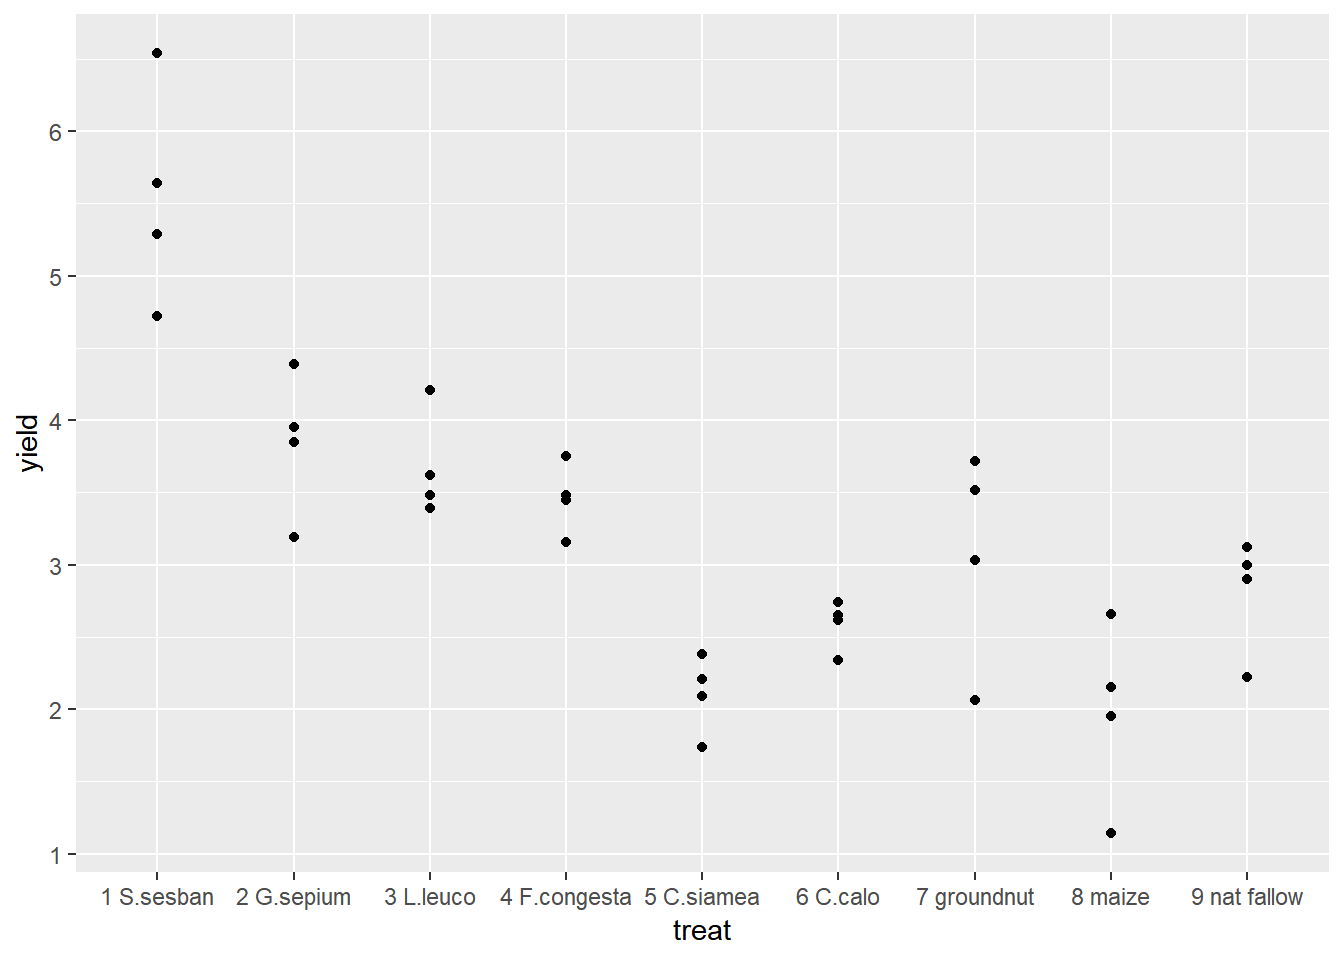
\includegraphics{bookdown-demo_files/figure-latex/unnamed-chunk-21-1.pdf}
We could also extend this to identify which points came from which reps.

\begin{Shaded}
\begin{Highlighting}[]
\KeywordTok{ggplot}\NormalTok{(}\DataTypeTok{data=}\NormalTok{fallow,}\KeywordTok{aes}\NormalTok{(}\DataTypeTok{y=}\NormalTok{yield,}\DataTypeTok{x=}\NormalTok{treat,}\DataTypeTok{col=}\NormalTok{rep))}\OperatorTok{+}\KeywordTok{geom_point}\NormalTok{()}
\end{Highlighting}
\end{Shaded}

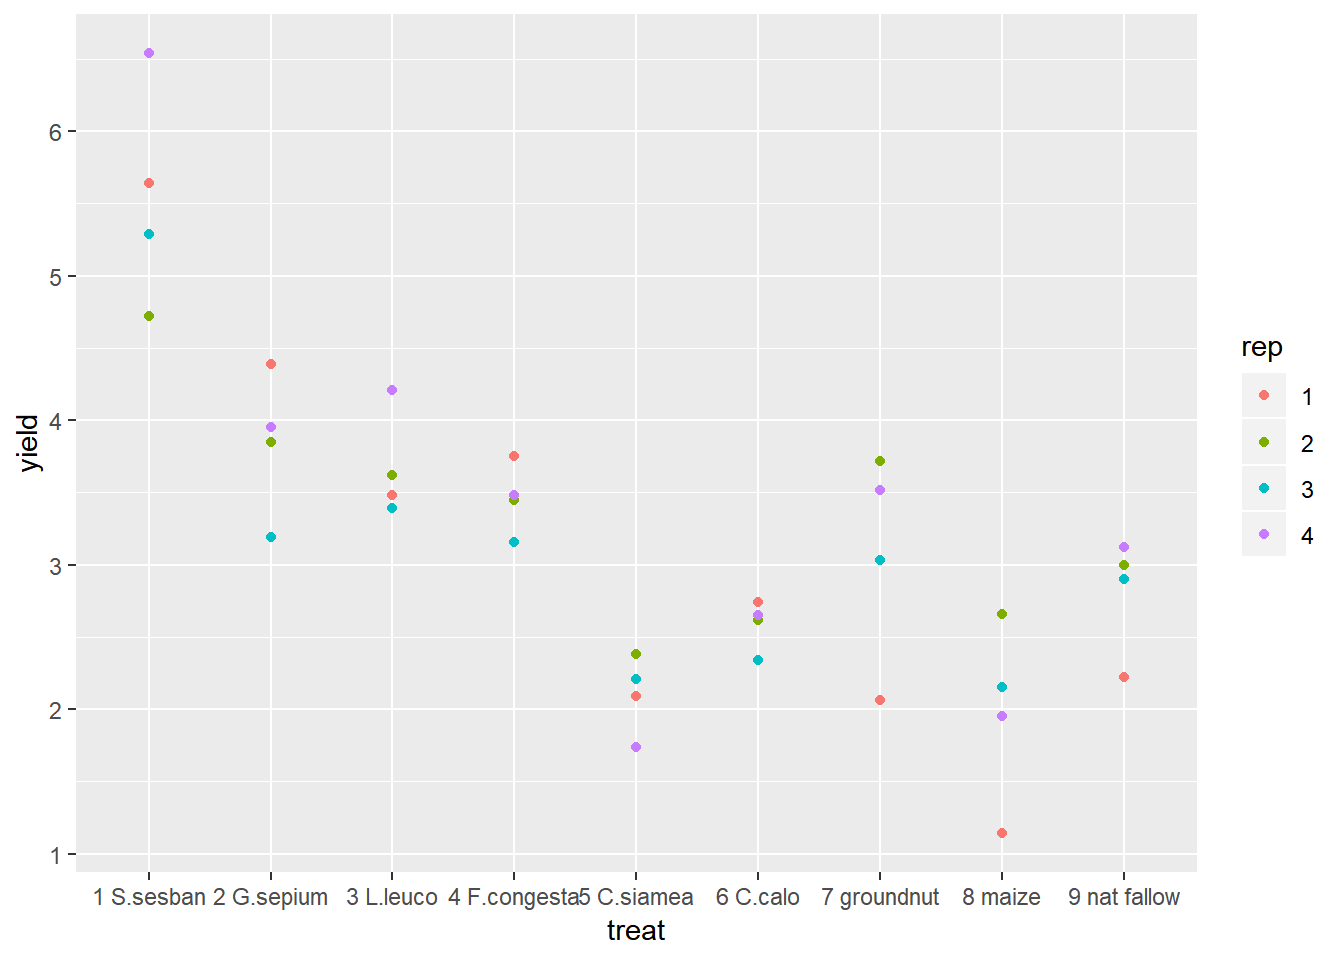
\includegraphics{bookdown-demo_files/figure-latex/unnamed-chunk-22-1.pdf}
Using ggplot2 we can easily change between different types of graph with
small changes to the code. Boxplots are very useful if we have lots of
data in each group, but in this example we only have 4 points so it is
easy to visualise all of our data using a scatter plot. But the only
change we would need to make to our original code is to change
geom\_point() to geom\_boxplot().

\begin{Shaded}
\begin{Highlighting}[]
\KeywordTok{ggplot}\NormalTok{(}\DataTypeTok{data=}\NormalTok{fallow,}\KeywordTok{aes}\NormalTok{(}\DataTypeTok{y=}\NormalTok{yield,}\DataTypeTok{x=}\NormalTok{treat))}\OperatorTok{+}\KeywordTok{geom_boxplot}\NormalTok{()}
\end{Highlighting}
\end{Shaded}

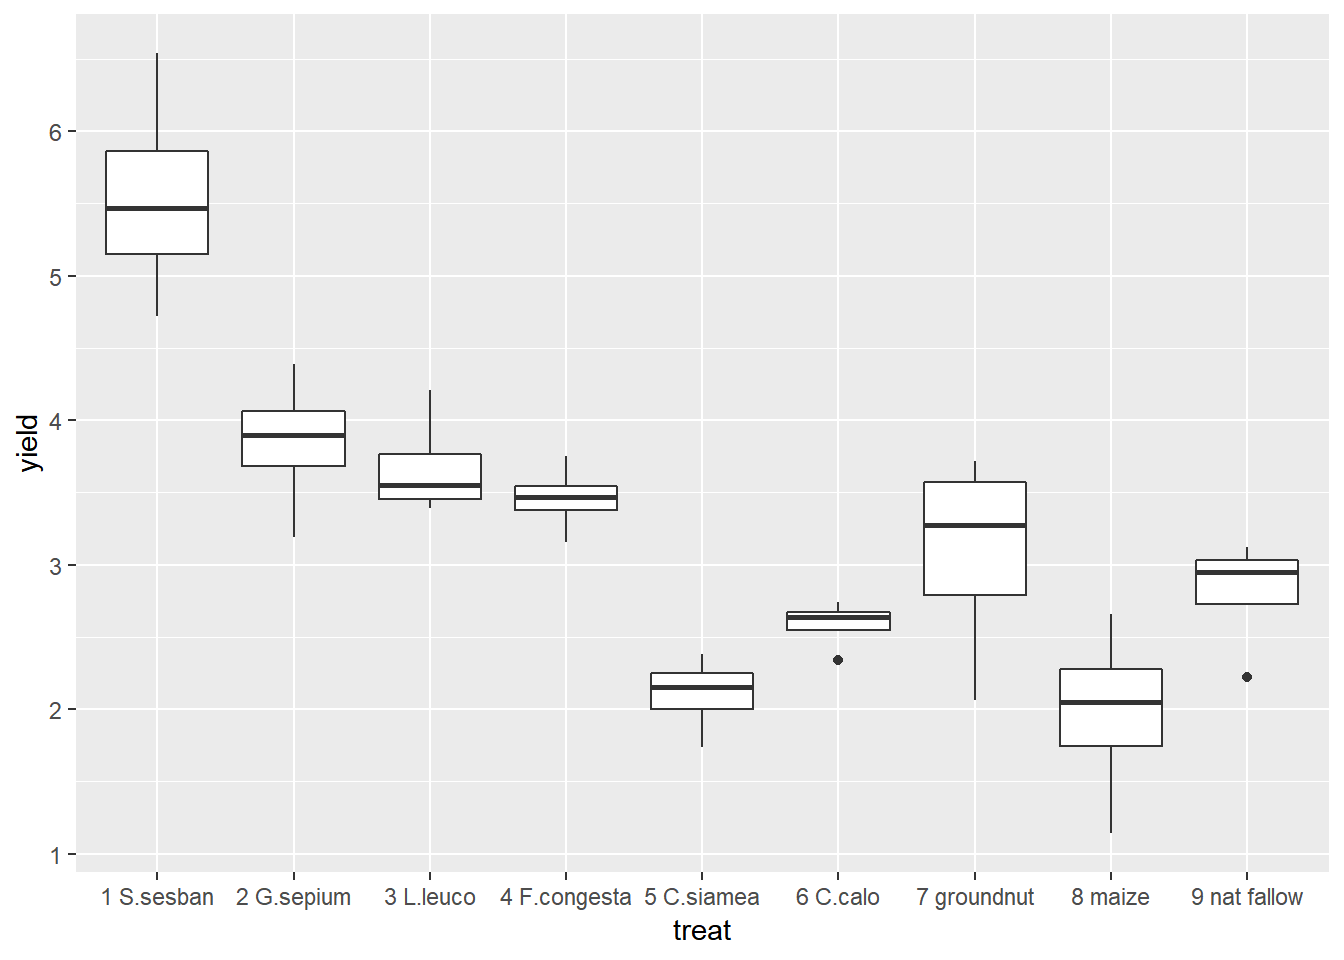
\includegraphics{bookdown-demo_files/figure-latex/unnamed-chunk-23-1.pdf}

From the figures produced we can see that treatment 1 has consistently
high yields. The lowest yield recorded for treatment 1 is higher than
the highest yield recorded for any of the other treatments. Treatments 5
and 8 had consistently low yields.

\subsubsection{Summary Statistics}\label{summary-statistics}

To produce summary statistics, by group, there are many options within
R. One option is to use the summaryBy function, from the doBy library.
The code used for this is quite similar to the code we will use to
produce models in a later step.

\begin{Shaded}
\begin{Highlighting}[]
\KeywordTok{summaryBy}\NormalTok{(yield}\OperatorTok{~}\NormalTok{treat, }\DataTypeTok{data=}\NormalTok{fallow, }\DataTypeTok{FUN=}\NormalTok{mean)}
\end{Highlighting}
\end{Shaded}

\begin{verbatim}
##          treat yield.mean
## 1   1 S.sesban     5.5475
## 2   2 G.sepium     3.8450
## 3    3 L.leuco     3.6750
## 4 4 F.congesta     3.4600
## 5   5 C.siamea     2.1050
## 6     6 C.calo     2.5875
## 7  7 groundnut     3.0825
## 8      8 maize     1.9750
## 9 9 nat fallow     2.8100
\end{verbatim}

We can also calculate multiple statistics in the same line of code

\begin{Shaded}
\begin{Highlighting}[]
\KeywordTok{summaryBy}\NormalTok{(yield}\OperatorTok{~}\NormalTok{treat, }\DataTypeTok{data=}\NormalTok{fallow, }\DataTypeTok{FUN=}\KeywordTok{c}\NormalTok{(min,max,mean,median,sd))}
\end{Highlighting}
\end{Shaded}

\begin{verbatim}
##          treat yield.min yield.max yield.mean yield.median  yield.sd
## 1   1 S.sesban      4.72      6.54     5.5475        5.465 0.7625997
## 2   2 G.sepium      3.19      4.39     3.8450        3.900 0.4956813
## 3    3 L.leuco      3.39      4.21     3.6750        3.550 0.3690077
## 4 4 F.congesta      3.16      3.75     3.4600        3.465 0.2412468
## 5   5 C.siamea      1.74      2.38     2.1050        2.150 0.2708628
## 6     6 C.calo      2.34      2.74     2.5875        2.635 0.1726992
## 7  7 groundnut      2.06      3.72     3.0825        3.275 0.7407372
## 8      8 maize      1.14      2.66     1.9750        2.050 0.6318491
## 9 9 nat fallow      2.22      3.12     2.8100        2.950 0.4034848
\end{verbatim}

\subsection{5. Specify a model for data}\label{specify-a-model-for-data}

In this design, an RCBD, we have one treatment factor, ``treat'', and
one layout factor ``rep''. More information about model fitting can be
found in section 2.

\begin{Shaded}
\begin{Highlighting}[]
\NormalTok{rcbdmodel1<-}\KeywordTok{lmer}\NormalTok{(yield}\OperatorTok{~}\NormalTok{treat}\OperatorTok{+}\NormalTok{(}\DecValTok{1}\OperatorTok{|}\NormalTok{rep),}\DataTypeTok{data=}\NormalTok{fallow)}
\end{Highlighting}
\end{Shaded}

R is unlike many other software packages in how it fits models. The best
way of handling models in R is to assign the model to a name (in this
case rcbdmodel1) and then ask R to provide different sorts of output for
this model. When you run the above line you will get now output from the
data - this is what we expected to see!

\subsection{6. Check the model}\label{check-the-model}

Before interpretting the model any further we should investigate the
model validity, to ensure any conclusions we draw are valid. There are 3
assumptions that we can check for using standard model checking plots.
1. Homogeneity (equal variance) 2. Values with high leverage 3.
Normality of residuals

The function plot() when used with a model will plot the fitted values
from the model against the expected values.

\begin{Shaded}
\begin{Highlighting}[]
\KeywordTok{plot}\NormalTok{(rcbdmodel1)}
\end{Highlighting}
\end{Shaded}

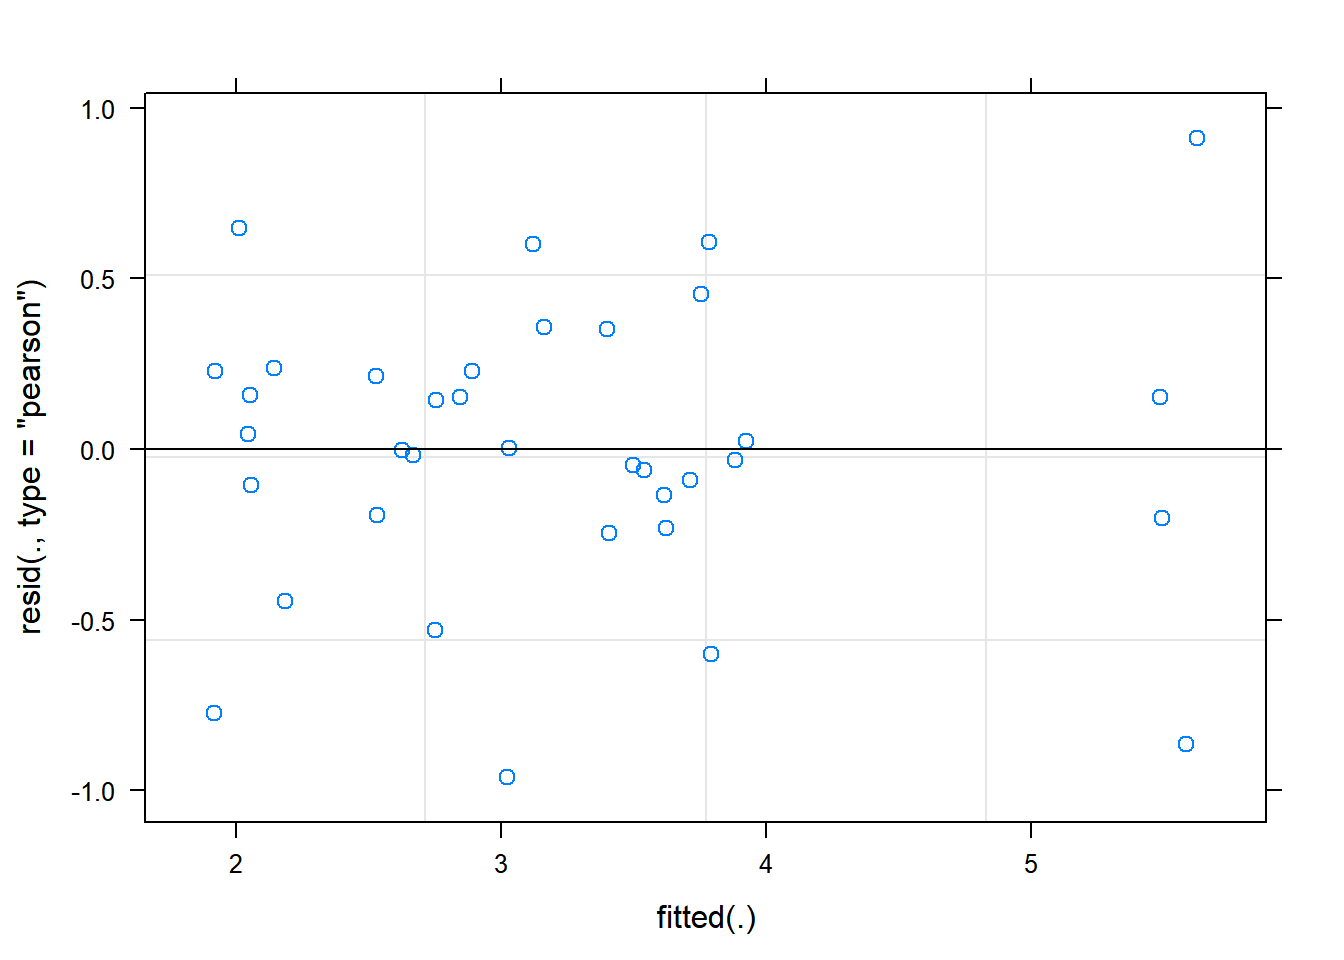
\includegraphics{bookdown-demo_files/figure-latex/unnamed-chunk-27-1.pdf}
The residual Vs fitted plot is a scatter plot of the Residuals on the
y-axis and the fitted on the x-axis and the aim for this plot is to test
the assumption of equal variance of the residuals across the range of
fitted values. Since the residuals do not funnel out (to form
triangular/diamond shape) the assumption of equal variance is met.

We can also see that there are no extreme values in the residuals which
might be potentially causing problems with the validity of our
conclusions (leverage)

To assess the assumption of normality we can produce a qqplot. This
shows us how closely the residuals follow a normal distribution - if
there are severe and syste,matic deviations from the line then we may
want to consider an alternative distribution.

\begin{Shaded}
\begin{Highlighting}[]
\KeywordTok{qqnorm}\NormalTok{(}\KeywordTok{resid}\NormalTok{(rcbdmodel1))}
\KeywordTok{qqline}\NormalTok{(}\KeywordTok{resid}\NormalTok{(rcbdmodel1))}
\end{Highlighting}
\end{Shaded}

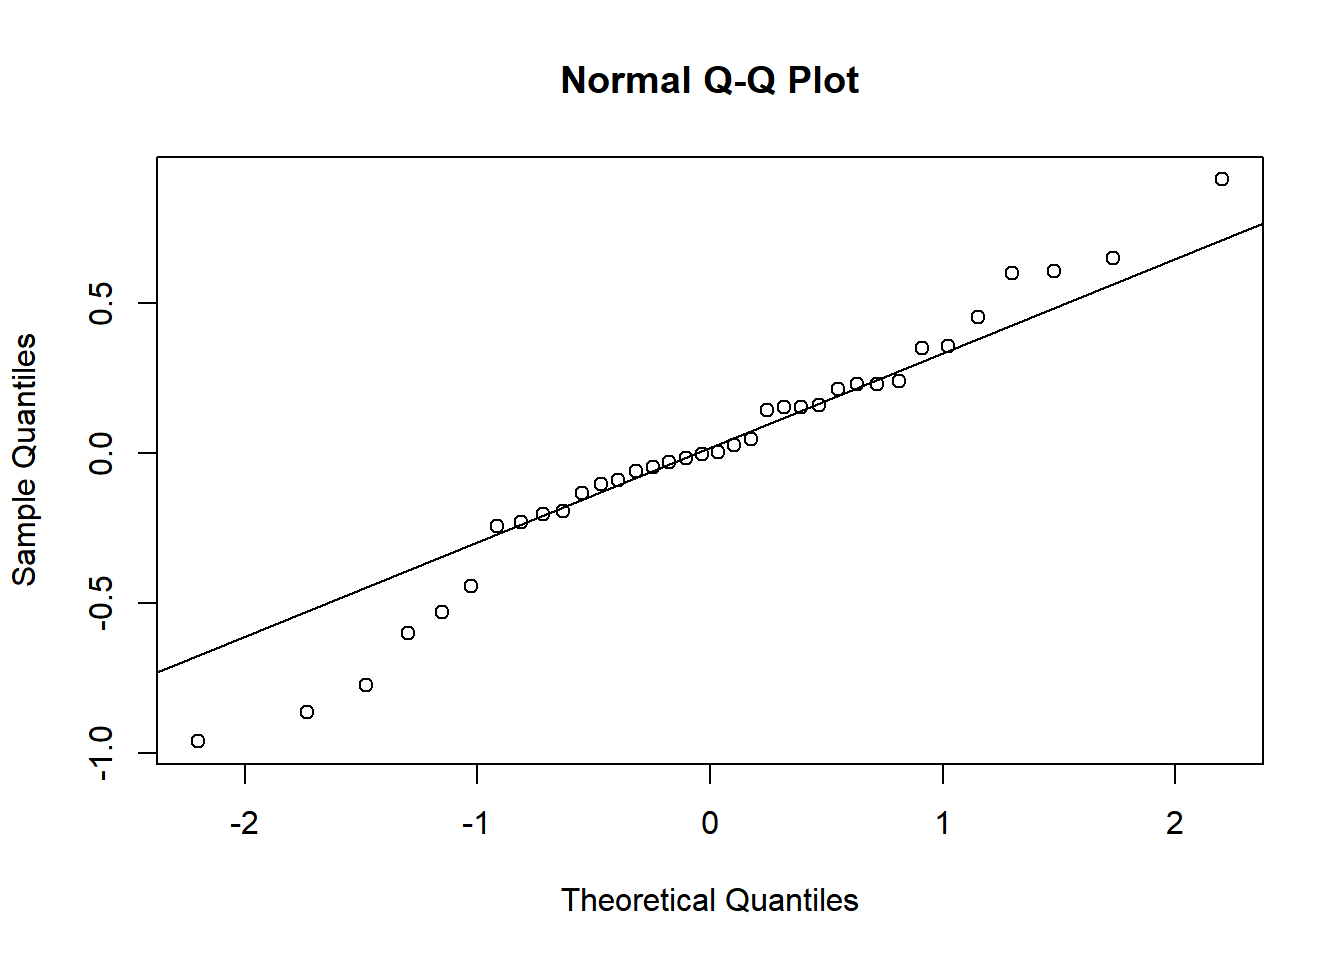
\includegraphics{bookdown-demo_files/figure-latex/unnamed-chunk-28-1.pdf}
In this case the residuals seem to fit the assumption required for
normality.

\subsection{7. Interpret Model}\label{interpret-model}

The anova() function only prints the rows of analysis of variance table
for treatment effects when looking at a mixed model fitted using lmer().

\begin{Shaded}
\begin{Highlighting}[]
\KeywordTok{anova}\NormalTok{(rcbdmodel1,}\DataTypeTok{ddf=}\StringTok{"Kenward-Roger"}\NormalTok{)}
\end{Highlighting}
\end{Shaded}

\begin{verbatim}
## Type III Analysis of Variance Table with Kenward-Roger's method
##       Sum Sq Mean Sq NumDF DenDF F value    Pr(>F)    
## treat 37.806  4.7258     8    24  20.146 6.981e-09 ***
## ---
## Signif. codes:  0 '***' 0.001 '**' 0.01 '*' 0.05 '.' 0.1 ' ' 1
\end{verbatim}

ddf=Kenward-Roger tells R which method to use for determining the
calculations of the table; this option matches the defaults found within
SAS or Genstat. The ANOVA table suggests a highly significant effect of
the treatment on the yield.

To obtain the residual variance, and the variance attributed to the
blocks we need an additional command. From these number it is possible
to reconstruct a more classic ANOVA table, if so desired.

\begin{Shaded}
\begin{Highlighting}[]
\KeywordTok{print}\NormalTok{(}\KeywordTok{VarCorr}\NormalTok{(rcbdmodel1), }\DataTypeTok{comp=}\NormalTok{(}\StringTok{"Variance"}\NormalTok{))}
\end{Highlighting}
\end{Shaded}

\begin{verbatim}
##  Groups   Name        Variance
##  rep      (Intercept) 0.013817
##  Residual             0.234577
\end{verbatim}

\subsection{8. Present the results from the
model}\label{present-the-results-from-the-model}

To help understand what the significant result from the ANOVA table
means we can produce several plots and tables to help us. First we can
use the function emmip() to produce plots of the modelled results,
including 95\% confidence intervals.

\begin{Shaded}
\begin{Highlighting}[]
\KeywordTok{emmip}\NormalTok{(rcbdmodel1,}\OperatorTok{~}\NormalTok{treat,}\DataTypeTok{CIs =} \OtherTok{TRUE}\NormalTok{)}
\end{Highlighting}
\end{Shaded}

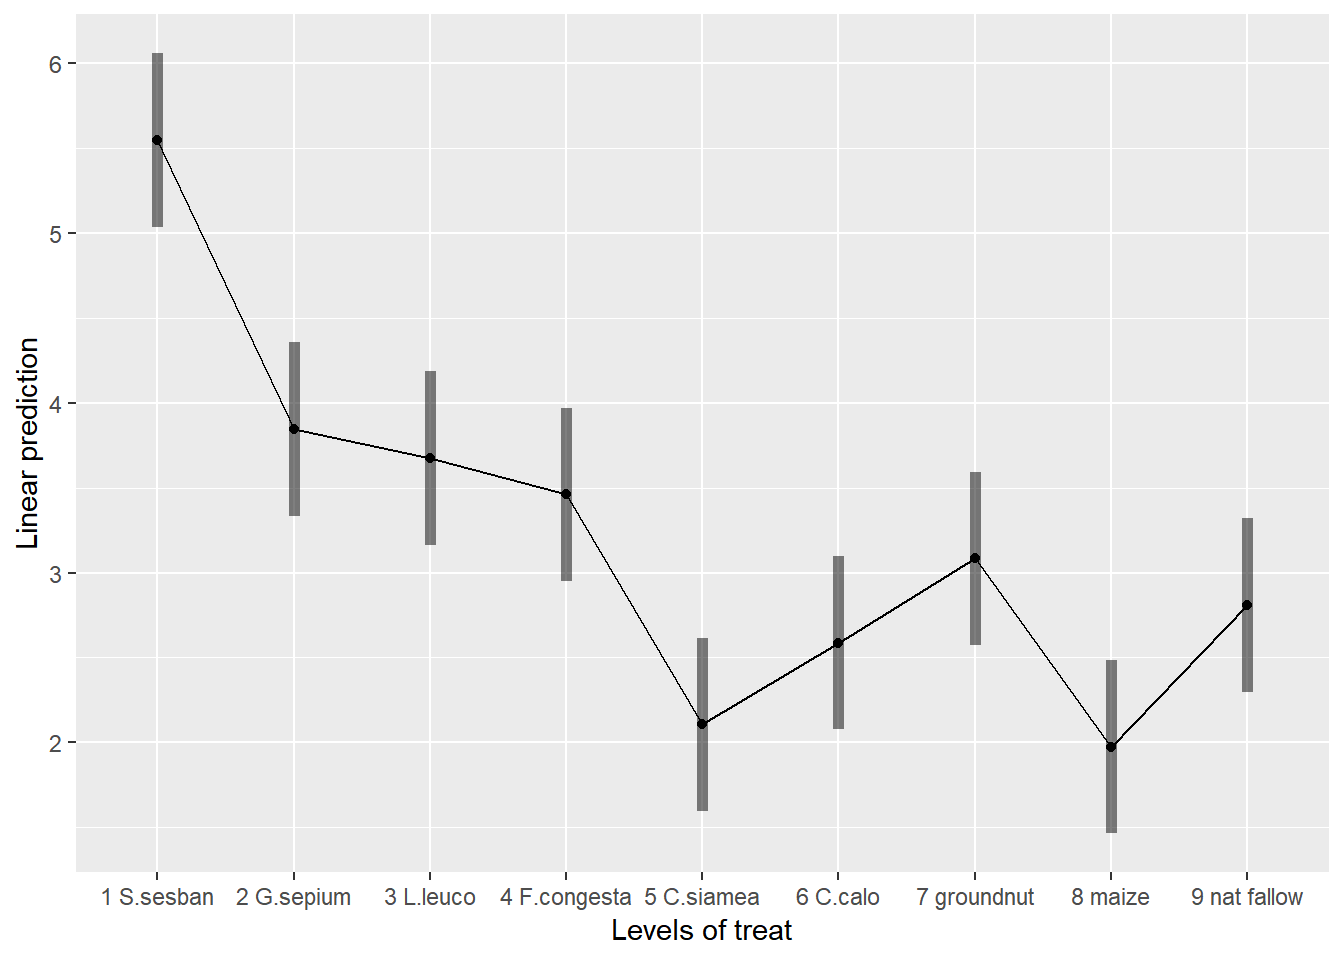
\includegraphics{bookdown-demo_files/figure-latex/unnamed-chunk-31-1.pdf}

To obtain the numbers used in creating this graph we can use the
function emmeans.

\begin{Shaded}
\begin{Highlighting}[]
\KeywordTok{emmeans}\NormalTok{(rcbdmodel1, }\OperatorTok{~}\NormalTok{treat)}
\end{Highlighting}
\end{Shaded}

\begin{verbatim}
##  treat        emmean        SE    df lower.CL upper.CL
##  1 S.sesban   5.5475 0.2491955 26.35   5.0356   6.0594
##  2 G.sepium   3.8450 0.2491955 26.35   3.3331   4.3569
##  3 L.leuco    3.6750 0.2491955 26.35   3.1631   4.1869
##  4 F.congesta 3.4600 0.2491955 26.35   2.9481   3.9719
##  5 C.siamea   2.1050 0.2491955 26.35   1.5931   2.6169
##  6 C.calo     2.5875 0.2491955 26.35   2.0756   3.0994
##  7 groundnut  3.0825 0.2491955 26.35   2.5706   3.5944
##  8 maize      1.9750 0.2491955 26.35   1.4631   2.4869
##  9 nat fallow 2.8100 0.2491955 26.35   2.2981   3.3219
## 
## Degrees-of-freedom method: kenward-roger 
## Confidence level used: 0.95
\end{verbatim}

And one method for conducting mean separation analysis we can use the
function cld().

\begin{Shaded}
\begin{Highlighting}[]
\KeywordTok{cld}\NormalTok{(}\KeywordTok{emmeans}\NormalTok{(rcbdmodel1, }\OperatorTok{~}\NormalTok{treat))}
\end{Highlighting}
\end{Shaded}

\begin{verbatim}
##  treat        emmean        SE    df lower.CL upper.CL .group
##  8 maize      1.9750 0.2491955 26.35   1.4631   2.4869  1    
##  5 C.siamea   2.1050 0.2491955 26.35   1.5931   2.6169  1    
##  6 C.calo     2.5875 0.2491955 26.35   2.0756   3.0994  12   
##  9 nat fallow 2.8100 0.2491955 26.35   2.2981   3.3219  123  
##  7 groundnut  3.0825 0.2491955 26.35   2.5706   3.5944  123  
##  4 F.congesta 3.4600 0.2491955 26.35   2.9481   3.9719   23  
##  3 L.leuco    3.6750 0.2491955 26.35   3.1631   4.1869   23  
##  2 G.sepium   3.8450 0.2491955 26.35   3.3331   4.3569    3  
##  1 S.sesban   5.5475 0.2491955 26.35   5.0356   6.0594     4 
## 
## Degrees-of-freedom method: kenward-roger 
## Confidence level used: 0.95 
## P value adjustment: tukey method for comparing a family of 9 estimates 
## significance level used: alpha = 0.05
\end{verbatim}

In the output, groups sharing a letter in the .group are not
statistically different from each other.

\section{Section 3 -- Methodological
Principles}\label{section-3-methodological-principles}

There are always many different ways of doing all that we have done here
in R. The less complex the method/code is, the better it is for you so
that you can easily grasp the method.

For instance, we have fitted our model as a linear mixed effect model
rather than traditional ANOVA because lmer model has the following
advantages:

\begin{enumerate}
\def\labelenumi{\arabic{enumi}.}
\tightlist
\item
  They are very flexible especially where we have repeated measures, for
  instance you don't need to have the same number of observations per
  subject/treatment.
\item
  Ability to account for a series of random effects. Not only are
  farms/farmers/plots\ldots{}. different from each other, but things
  with in farms/plots\ldots{}.. also differ . Not taking these sources
  of variation into account will lead to underestimations of accuracy.
\item
  Allows for generalization of non-normal data.\\
\item
  Handling missing data: If the percentage of missing data is small and
  that data missing is a random sample of the data set,data from the
  observations with missing data can be analysed with lmer (unlike other
  packages that would do listwise deletion.
\item
  Takes into account variation that is explained by the predictor
  variables of interest ie fixed effects and variation that is not
  explained by these predictors ie random effects.
\end{enumerate}

Not forgetting that selecting variables to include in our model
generally depends on theory, statistics and practical knowledge the
following (general) rules will be considered while fitting our models:

\begin{enumerate}
\def\labelenumi{\roman{enumi})}
\tightlist
\item
  Consider the Treatments (A, B,\ldots{}.) as fixed effects and hence
  presented as A*B in our model.
\item
  Consider the layout factors as random effects and hence presented as
  (1\textbar{}block/plot\ldots{}) in our model. Generally, our model is
  in the form of Model\textless{}-lmer(Response\textasciitilde{}
  (1\textbar{}Block/Plot)+Treatment A + Treatment B\ldots{},
  data=Dataframe)
\end{enumerate}

In this example using the fallow data, note that if we had a
``completely randomised'' design rather than a ``blocked randomised
design'', where each treatment was replicated 4 times but there were not
blocks, this is a rare example of a design which cannot be handled by
lmer. In this case there would be no random effects, so the function
needed would be lm() rather than lmer().

Food for thought: Your best model will certainly be as good as the data
you collected!!!

\chapter{Split Plot Designs}\label{split-plot-designs}

Aim: make it easy to do standard analysis of standard experimental
designs used in field trials Assumptions: you know some basic R, have R
and RStudio already installed on your compuiter and you are familiar
with the standard analyses of field trials.\\
This document will focus initially on the simple analysis of a split
plot design trial using R. Section 1 provides the steps used to produce
the analysis; Section 2 provides some commentary on how these commands
work, what output is created, and why these commadns were chosen;
Section 3 deals with aspects of the statistical methodology.

It would be beneficial to also read through Part 1 in this series,
analysis of RCBD single factor experiments. You may notice many
similarities in the R syntax used in these guides.

\section{About the data}\label{about-the-data-1}

The data for this example involves a split plot designed experiment.
Treatments are 4 cropping patterns, and two nitrogen levels. The design
is a split Both N and P could limit maize growth in the --N subplots,
whereas N will not limit maize growth in the +N subplots. The comparison
of +N and --N subplots within a mainplot will assess whether the fallows
have eliminated N deficiency for maize.

Differences in maize yield among treatments for the +N subplot will
result from differences in P plus ``fallow benefits'' to maize.
Differences in maize yield among treatments for the -N subplot will
result from differences in N plus P plus ``fallow benefits'' to maize.

The following steps were followed to generate the output in this
document. The data was organized in excel rectangle columns with the
different variables appearing in excel columns. All data checks were
done in excel, meaningful data was selected and a copy of this data file
was stored as a CSV file to make data import easy in R. The data file
used in this analysis can be downloaded here:
\url{https://bit.ly/2rfLBEt}

\section{Section 1: Steps in analysis using
R}\label{section-1-steps-in-analysis-using-r-1}

\begin{enumerate}
\def\labelenumi{\arabic{enumi}.}
\tightlist
\item
  Install R packages needed
\end{enumerate}

\begin{Shaded}
\begin{Highlighting}[]
\KeywordTok{library}\NormalTok{(ggplot2)}
\KeywordTok{library}\NormalTok{(emmeans)}
\KeywordTok{library}\NormalTok{(doBy)}
\KeywordTok{library}\NormalTok{(lmerTest)}
\KeywordTok{library}\NormalTok{(multcompView)}
\end{Highlighting}
\end{Shaded}

\begin{enumerate}
\def\labelenumi{\arabic{enumi}.}
\setcounter{enumi}{1}
\tightlist
\item
  Import data
\end{enumerate}

\begin{Shaded}
\begin{Highlighting}[]
\NormalTok{fphosphorus  <-}\StringTok{ }\KeywordTok{read.csv}\NormalTok{(}\StringTok{"C:/Users/Admin/Desktop/FPhosphorus.csv"}\NormalTok{)}
\end{Highlighting}
\end{Shaded}

\begin{enumerate}
\def\labelenumi{\arabic{enumi}.}
\setcounter{enumi}{2}
\tightlist
\item
  Check and update data
\end{enumerate}

\begin{Shaded}
\begin{Highlighting}[]
\KeywordTok{summary}\NormalTok{(fphosphorus)}
\KeywordTok{str}\NormalTok{(fphosphorus)}

\NormalTok{fphosphorus}\OperatorTok{$}\NormalTok{mainplot<-}\KeywordTok{factor}\NormalTok{(fphosphorus}\OperatorTok{$}\NormalTok{mainplot)}
\NormalTok{fphosphorus}\OperatorTok{$}\NormalTok{subplot<-}\KeywordTok{factor}\NormalTok{(fphosphorus}\OperatorTok{$}\NormalTok{subplot)}
\NormalTok{fphosphorus}\OperatorTok{$}\NormalTok{block<-}\KeywordTok{factor}\NormalTok{(fphosphorus}\OperatorTok{$}\NormalTok{block)}
\end{Highlighting}
\end{Shaded}

\begin{enumerate}
\def\labelenumi{\arabic{enumi}.}
\setcounter{enumi}{3}
\tightlist
\item
  Explore data
\end{enumerate}

\begin{Shaded}
\begin{Highlighting}[]
\KeywordTok{ggplot}\NormalTok{(}\DataTypeTok{data=}\NormalTok{fphosphorus,}\KeywordTok{aes}\NormalTok{(}\DataTypeTok{y=}\NormalTok{grain,}\DataTypeTok{x=}\NormalTok{fallow))}\OperatorTok{+}\KeywordTok{geom_boxplot}\NormalTok{(}\KeywordTok{aes}\NormalTok{(}\DataTypeTok{colour=}\NormalTok{nitrogen))}
\KeywordTok{summaryBy}\NormalTok{(grain}\OperatorTok{~}\NormalTok{fallow}\OperatorTok{+}\NormalTok{nitrogen, }\DataTypeTok{data=}\NormalTok{fphosphorus, }\DataTypeTok{FUN=}\KeywordTok{c}\NormalTok{(mean,sd))}
\end{Highlighting}
\end{Shaded}

\begin{enumerate}
\def\labelenumi{\arabic{enumi}.}
\setcounter{enumi}{4}
\tightlist
\item
  Specify a model for data
\end{enumerate}

\begin{Shaded}
\begin{Highlighting}[]
\NormalTok{splitplotmodel1<-}\KeywordTok{lmer}\NormalTok{(grain}\OperatorTok{~}\NormalTok{fallow}\OperatorTok{*}\NormalTok{nitrogen}\OperatorTok{+}\NormalTok{(}\DecValTok{1}\OperatorTok{|}\NormalTok{block}\OperatorTok{/}\NormalTok{mainplot), }\DataTypeTok{data=}\NormalTok{fphosphorus)}
\end{Highlighting}
\end{Shaded}

\begin{enumerate}
\def\labelenumi{\arabic{enumi}.}
\setcounter{enumi}{5}
\tightlist
\item
  Check the model
\end{enumerate}

\begin{Shaded}
\begin{Highlighting}[]
\KeywordTok{plot}\NormalTok{(splitplotmodel1)}

\KeywordTok{qqnorm}\NormalTok{(}\KeywordTok{resid}\NormalTok{(splitplotmodel1))}
\KeywordTok{qqline}\NormalTok{(}\KeywordTok{resid}\NormalTok{(splitplotmodel1))}

\NormalTok{splitplotmodel2<-}\KeywordTok{lmer}\NormalTok{(}\KeywordTok{sqrt}\NormalTok{(grain)}\OperatorTok{~}\NormalTok{fallow}\OperatorTok{*}\NormalTok{nitrogen}\OperatorTok{+}\NormalTok{(}\DecValTok{1}\OperatorTok{|}\NormalTok{block}\OperatorTok{/}\NormalTok{mainplot), }\DataTypeTok{data=}\NormalTok{fphosphorus)}

\KeywordTok{plot}\NormalTok{(splitplotmodel2)}

\KeywordTok{qqnorm}\NormalTok{(}\KeywordTok{resid}\NormalTok{(splitplotmodel2))}
\KeywordTok{qqline}\NormalTok{(}\KeywordTok{resid}\NormalTok{(splitplotmodel2))}
\end{Highlighting}
\end{Shaded}

\begin{enumerate}
\def\labelenumi{\arabic{enumi}.}
\setcounter{enumi}{6}
\tightlist
\item
  Interpret the model
\end{enumerate}

\begin{Shaded}
\begin{Highlighting}[]
\KeywordTok{anova}\NormalTok{(splitplotmodel2, }\DataTypeTok{ddf=}\StringTok{"Kenward-Roger"}\NormalTok{)}
\KeywordTok{print}\NormalTok{(}\KeywordTok{VarCorr}\NormalTok{(splitplotmodel2), }\DataTypeTok{comp=}\NormalTok{(}\StringTok{"Variance"}\NormalTok{))}
\end{Highlighting}
\end{Shaded}

\begin{enumerate}
\def\labelenumi{\arabic{enumi}.}
\setcounter{enumi}{7}
\tightlist
\item
  Present the results from the model
\end{enumerate}

\begin{Shaded}
\begin{Highlighting}[]
\KeywordTok{emmip}\NormalTok{(splitplotmodel2,nitrogen}\OperatorTok{~}\NormalTok{fallow,}\DataTypeTok{CIs =} \OtherTok{TRUE}\NormalTok{,}\DataTypeTok{type=}\StringTok{"response"}\NormalTok{)}
\KeywordTok{emmeans}\NormalTok{(splitplotmodel2,}\OperatorTok{~}\NormalTok{fallow,}\DataTypeTok{type=}\StringTok{"response"}\NormalTok{)}
\KeywordTok{cld}\NormalTok{(}\KeywordTok{emmeans}\NormalTok{(splitplotmodel2,}\OperatorTok{~}\NormalTok{fallow,}\DataTypeTok{type=}\StringTok{"response"}\NormalTok{))}
\end{Highlighting}
\end{Shaded}

\section{Section 2: Explanation of
Steps}\label{section-2-explanation-of-steps-1}

\subsection{1. Install R packages
needed}\label{install-r-packages-needed-1}

A number of packages following packages were used during data
exploration and analysis. For a general introduction explaining what R
packages are and how they work, this is a really useful guide
\url{https://www.datacamp.com/community/tutorials/r-packages-guide}. For
each of these packages to be installed, using install.packages(), this
requires a reliable internet connection and a correctly installed
version of R and RStudio. If you are having difficulties installing
these packages please ask for help.

\begin{Shaded}
\begin{Highlighting}[]
\KeywordTok{install.packages}\NormalTok{(}\StringTok{"ggplot2"}\NormalTok{)}
\KeywordTok{library}\NormalTok{(ggplot2)}
\end{Highlighting}
\end{Shaded}

\texttt{ggplot2} This package provides a powerful graphics language for
creating elegant and complex graphs in R.

\begin{Shaded}
\begin{Highlighting}[]
\KeywordTok{install.packages}\NormalTok{(}\StringTok{"emmeans"}\NormalTok{)}
\KeywordTok{library}\NormalTok{(emmeans)}
\end{Highlighting}
\end{Shaded}

\texttt{emmeans} Estimated marginal means (also known as least squares
means) helps provide expected mean values and confidence intervals from
statistical models.

\begin{Shaded}
\begin{Highlighting}[]
\KeywordTok{install.packages}\NormalTok{(}\StringTok{"doBy"}\NormalTok{)}
\KeywordTok{library}\NormalTok{(doBy)}
\end{Highlighting}
\end{Shaded}

\texttt{doBy}Allows easy production of summary statistic tables

\begin{Shaded}
\begin{Highlighting}[]
\KeywordTok{install.packages}\NormalTok{(}\StringTok{"lmerTest"}\NormalTok{)}
\KeywordTok{library}\NormalTok{(lmerTest)}
\end{Highlighting}
\end{Shaded}

\texttt{lmerTest} Allows produce of flexible mixed effects regression
models, similar to REML in Genstat.

\begin{Shaded}
\begin{Highlighting}[]
\KeywordTok{install.packages}\NormalTok{(}\StringTok{"multcompView"}\NormalTok{)}
\KeywordTok{library}\NormalTok{(multcompView)}
\end{Highlighting}
\end{Shaded}

\texttt{multcompView} allows for mean seperation methods on analyses

\subsection{2. Import data}\label{import-data-1}

Our data set saved as a CSV file, so we can use the read.csv commmand to
import the data. We are going to assign the name of the data with R to
be \texttt{fphosphorus}. Remember in R Studio you could also use the
``Import Dataset'' menu to import a dataset.

\begin{Shaded}
\begin{Highlighting}[]
\NormalTok{fphosphorus  <-}\StringTok{ }\KeywordTok{read.csv}\NormalTok{(}\StringTok{"C:/Users/Admin/Desktop/FPhosphorus.csv"}\NormalTok{)}
\end{Highlighting}
\end{Shaded}

\subsection{3. Check and update data}\label{check-and-update-data-1}

When reading data into R it is always useful to check that data is in
the format expected. How many variables are there? How many rows? How
have the columns been read in? The summary command can help to show if
the data is being treated correctly.

\begin{Shaded}
\begin{Highlighting}[]
\KeywordTok{summary}\NormalTok{(fphosphorus)}
\end{Highlighting}
\end{Shaded}

\begin{verbatim}
##      farmer       block      mainplot       subplot   
##  BTS-10 : 8   Min.   :1   Min.   :1.00   Min.   :1.0  
##  BTS-10B: 8   1st Qu.:3   1st Qu.:1.75   1st Qu.:1.0  
##  BTS-18 : 8   Median :5   Median :2.50   Median :1.5  
##  BTS-25 : 8   Mean   :5   Mean   :2.50   Mean   :1.5  
##  BTS-27 : 8   3rd Qu.:7   3rd Qu.:3.25   3rd Qu.:2.0  
##  BTS-32 : 8   Max.   :9   Max.   :4.00   Max.   :2.0  
##  (Other):24                                           
##              fallow   nitrogen     grain         striga1       
##  Continous Maize:18   No :36   Min.   :0.00   Min.   :   7.00  
##  Crotolaria     :18   Yes:36   1st Qu.:0.60   1st Qu.:  86.75  
##  Tephrosia      :18            Median :1.25   Median : 323.50  
##  Tithonia       :18            Mean   :1.70   Mean   : 582.04  
##                                3rd Qu.:2.40   3rd Qu.: 852.25  
##                                Max.   :5.30   Max.   :2999.00  
##                                                                
##     striga2           striga3          striga4      
##  Min.   :   2.00   Min.   :   0.0   Min.   :   0.0  
##  1st Qu.:  13.75   1st Qu.:  10.0   1st Qu.:  17.0  
##  Median : 137.50   Median :  29.5   Median : 172.0  
##  Mean   : 566.11   Mean   :  84.4   Mean   : 337.7  
##  3rd Qu.: 926.00   3rd Qu.:  78.5   3rd Qu.: 448.5  
##  Max.   :2645.00   Max.   :1208.0   Max.   :1406.0  
##                                     NA's   :32
\end{verbatim}

Where data is being treated as a numeric variable (i.e.~a number)
\texttt{summary} provides statistics like the mean, min and max. Where
data is being treated like a categorical variable (i.e.~a group) then
summary provides frequency tables.

From the results we can see that the variables block, mainplor and
subplot are being considered as numeric variables. However these are
grouping variables, not number variables, the numbers used are simply
codes. If we do not rectify this then our analysis later will be
incorrect and meaningless.\\
This can also be seen more explicitly using the str() function.

\begin{Shaded}
\begin{Highlighting}[]
\KeywordTok{str}\NormalTok{(fphosphorus)}
\end{Highlighting}
\end{Shaded}

\begin{verbatim}
## 'data.frame':    72 obs. of  11 variables:
##  $ farmer  : Factor w/ 9 levels "BTS-10","BTS-10B",..: 1 1 1 1 1 1 1 1 2 2 ...
##  $ block   : int  7 7 7 7 7 7 7 7 8 8 ...
##  $ mainplot: int  1 1 2 2 3 3 4 4 1 1 ...
##  $ subplot : int  1 2 1 2 1 2 1 2 1 2 ...
##  $ fallow  : Factor w/ 4 levels "Continous Maize",..: 1 1 4 4 2 2 3 3 3 3 ...
##  $ nitrogen: Factor w/ 2 levels "No","Yes": 1 2 2 1 2 1 2 1 1 2 ...
##  $ grain   : num  0.8 3 2.2 2.4 1.2 3 0.9 4.1 0.4 0.5 ...
##  $ striga1 : int  1438 1340 482 340 98 90 232 120 2854 1715 ...
##  $ striga2 : int  1736 960 2092 660 680 921 2645 1033 1709 941 ...
##  $ striga3 : int  37 16 63 32 15 57 57 95 12 24 ...
##  $ striga4 : int  NA NA NA NA NA NA NA NA NA NA ...
\end{verbatim}

So we need to convert these variables into factors.

\begin{Shaded}
\begin{Highlighting}[]
\NormalTok{fphosphorus}\OperatorTok{$}\NormalTok{block<-}\KeywordTok{factor}\NormalTok{(fphosphorus}\OperatorTok{$}\NormalTok{block)}
\NormalTok{fphosphorus}\OperatorTok{$}\NormalTok{mainplot<-}\KeywordTok{factor}\NormalTok{(fphosphorus}\OperatorTok{$}\NormalTok{mainplot)}
\NormalTok{fphosphorus}\OperatorTok{$}\NormalTok{subplot<-}\KeywordTok{factor}\NormalTok{(fphosphorus}\OperatorTok{$}\NormalTok{subplot)}
\end{Highlighting}
\end{Shaded}

These commands take the column block within the data frame fphosphorus,
converts into a factor and saves the result in a column called block
within fphosphorus

\subsection{4. Explore data}\label{explore-data-1}

\subsection{Plots}\label{plots-1}

In Tutorial 1 we produced plots showing all of the data plotted as
points, like this:

\begin{Shaded}
\begin{Highlighting}[]
\KeywordTok{ggplot}\NormalTok{(}\DataTypeTok{data=}\NormalTok{fphosphorus,}\KeywordTok{aes}\NormalTok{(}\DataTypeTok{y=}\NormalTok{grain,}\DataTypeTok{x=}\NormalTok{fallow,}\DataTypeTok{colour=}\NormalTok{nitrogen))}\OperatorTok{+}\KeywordTok{geom_point}\NormalTok{()}
\end{Highlighting}
\end{Shaded}

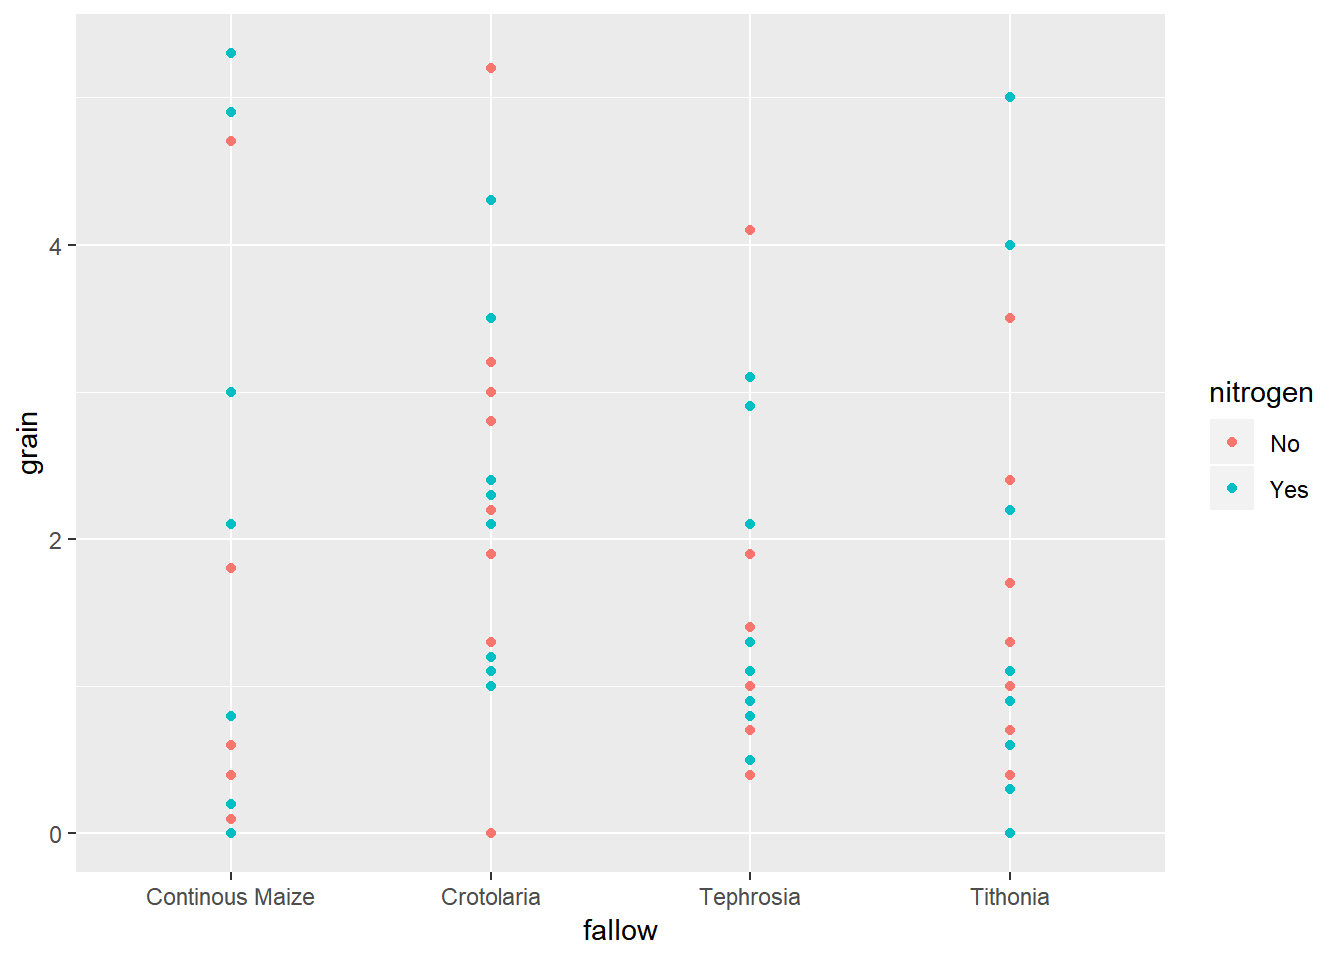
\includegraphics{bookdown-demo_files/figure-latex/unnamed-chunk-53-1.pdf}
But in this instance there are too many points to be able to fully
understand how the results are distributed. In this case we would get
better information through looking at some boxplots.

\begin{Shaded}
\begin{Highlighting}[]
\KeywordTok{ggplot}\NormalTok{(}\DataTypeTok{data=}\NormalTok{fphosphorus,}\KeywordTok{aes}\NormalTok{(}\DataTypeTok{y=}\NormalTok{grain,}\DataTypeTok{x=}\NormalTok{fallow,}\DataTypeTok{colour=}\NormalTok{nitrogen))}\OperatorTok{+}\KeywordTok{geom_boxplot}\NormalTok{()}
\end{Highlighting}
\end{Shaded}

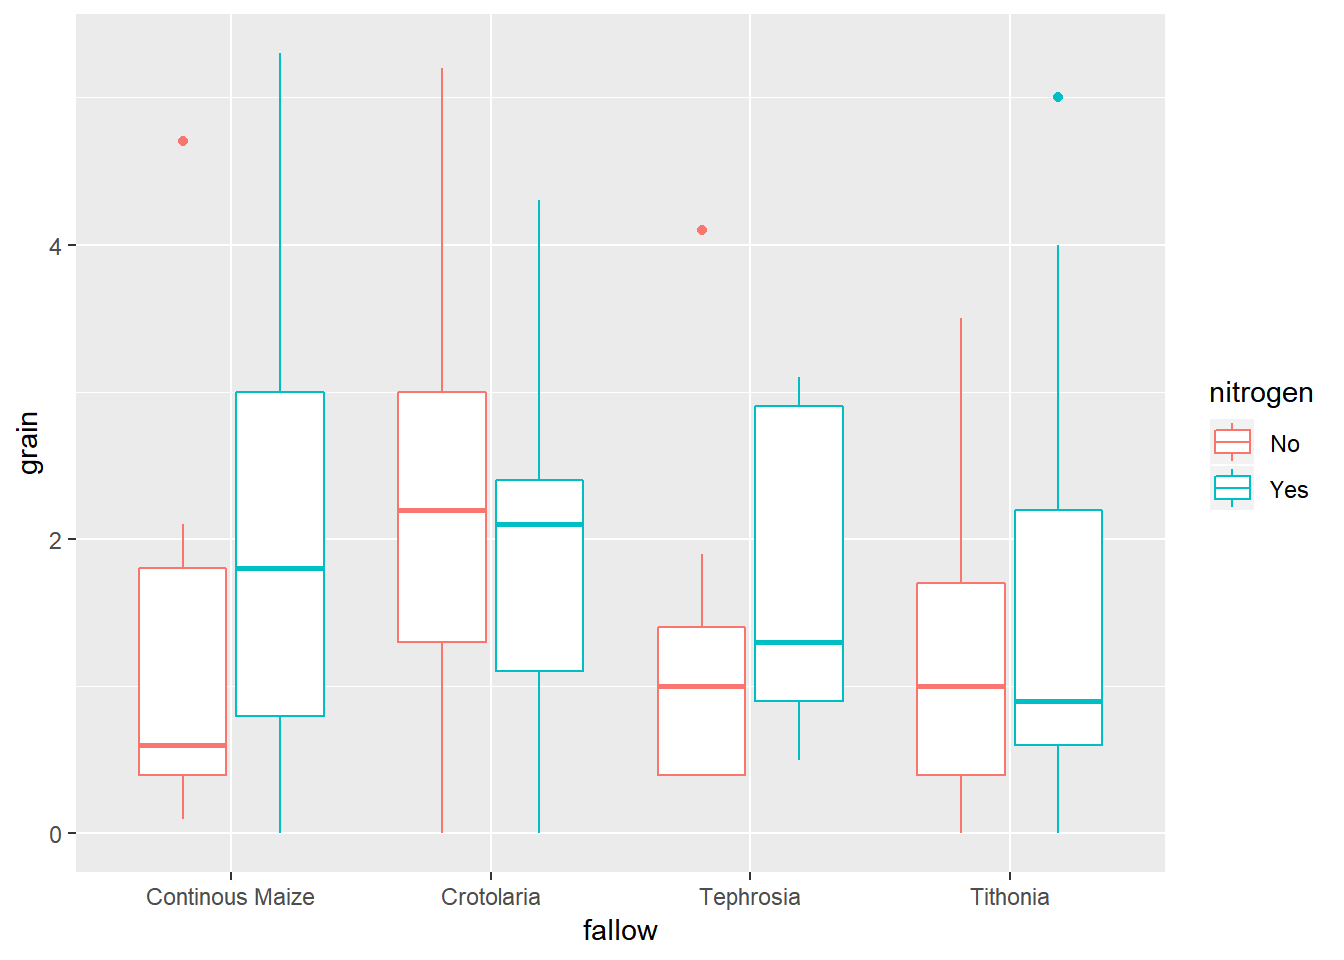
\includegraphics{bookdown-demo_files/figure-latex/unnamed-chunk-54-1.pdf}

\subsection{Summary Statistics}\label{summary-statistics-1}

Using the summaryBy() function makes it easy to split summary statsitics
into groups based on more than one factor. So the combination of fallow
treatment and nitrogen treatment can be obtained using a + sign between
the two variables.

\begin{Shaded}
\begin{Highlighting}[]
\KeywordTok{summaryBy}\NormalTok{(grain}\OperatorTok{~}\NormalTok{fallow}\OperatorTok{+}\NormalTok{nitrogen, }\DataTypeTok{data=}\NormalTok{fphosphorus, }\DataTypeTok{FUN=}\KeywordTok{c}\NormalTok{(mean,sd))}
\end{Highlighting}
\end{Shaded}

\begin{verbatim}
##            fallow nitrogen grain.mean grain.sd
## 1 Continous Maize       No   1.277778 1.446356
## 2 Continous Maize      Yes   2.100000 1.948718
## 3      Crotolaria       No   2.322222 1.475447
## 4      Crotolaria      Yes   1.988889 1.334583
## 5       Tephrosia       No   1.255556 1.181219
## 6       Tephrosia      Yes   1.733333 1.024695
## 7        Tithonia       No   1.255556 1.125956
## 8        Tithonia      Yes   1.666667 1.736376
\end{verbatim}

\subsection{5. Specify a model for
data}\label{specify-a-model-for-data-1}

In this design, a split plot desin, we have two treatment factors,
``fallow'' and ``nitrogen'', and two layout factors ``block'' and
``mainplot''.

In order to test the ``main effects'' of the treatmetns as well as the
interaction between the two factors, then we need to make sure the
formula is specified as factor1*factor2. Using factor1+factor2 will only
include the main effects and not include the interaction.

When dealing with the split plot design, across multiple blocks, then
the random effects need to be nested hierachically, from biggest down to
smallest. This is done with a random effect that includes a / and looks
like (1\textbar{}biggestlayoutunit/nextbiggestlayout unit).

So the model we want to fit therefore looks like:

\begin{Shaded}
\begin{Highlighting}[]
\NormalTok{splitplotmodel1<-}\KeywordTok{lmer}\NormalTok{(grain}\OperatorTok{~}\NormalTok{fallow}\OperatorTok{*}\NormalTok{nitrogen}\OperatorTok{+}\NormalTok{(}\DecValTok{1}\OperatorTok{|}\NormalTok{block}\OperatorTok{/}\NormalTok{mainplot), }\DataTypeTok{data=}\NormalTok{fphosphorus)}
\end{Highlighting}
\end{Shaded}

R is unlike many other software packages in how it fits models. The best
way of handling models in R is to assign the model to a name (in this
case rcbdmodel1) and then ask R to provide different sorts of output for
this model. When you run the above line you will get now output from the
data - this is what we expected to see!

\subsection{6. Check the model}\label{check-the-model-1}

Before interpretting the model any further we should investigate the
model validity, to ensure any conclusions we draw are valid. There are 3
assumptions that we can check for using standard model checking plots.
1. Homogeneity (equal variance) 2. Values with high leverage 3.
Normality of residuals

The function plot() when used with a model will plot the fitted values
from the model against the expected values.

\begin{Shaded}
\begin{Highlighting}[]
\KeywordTok{plot}\NormalTok{(splitplotmodel1)}
\end{Highlighting}
\end{Shaded}

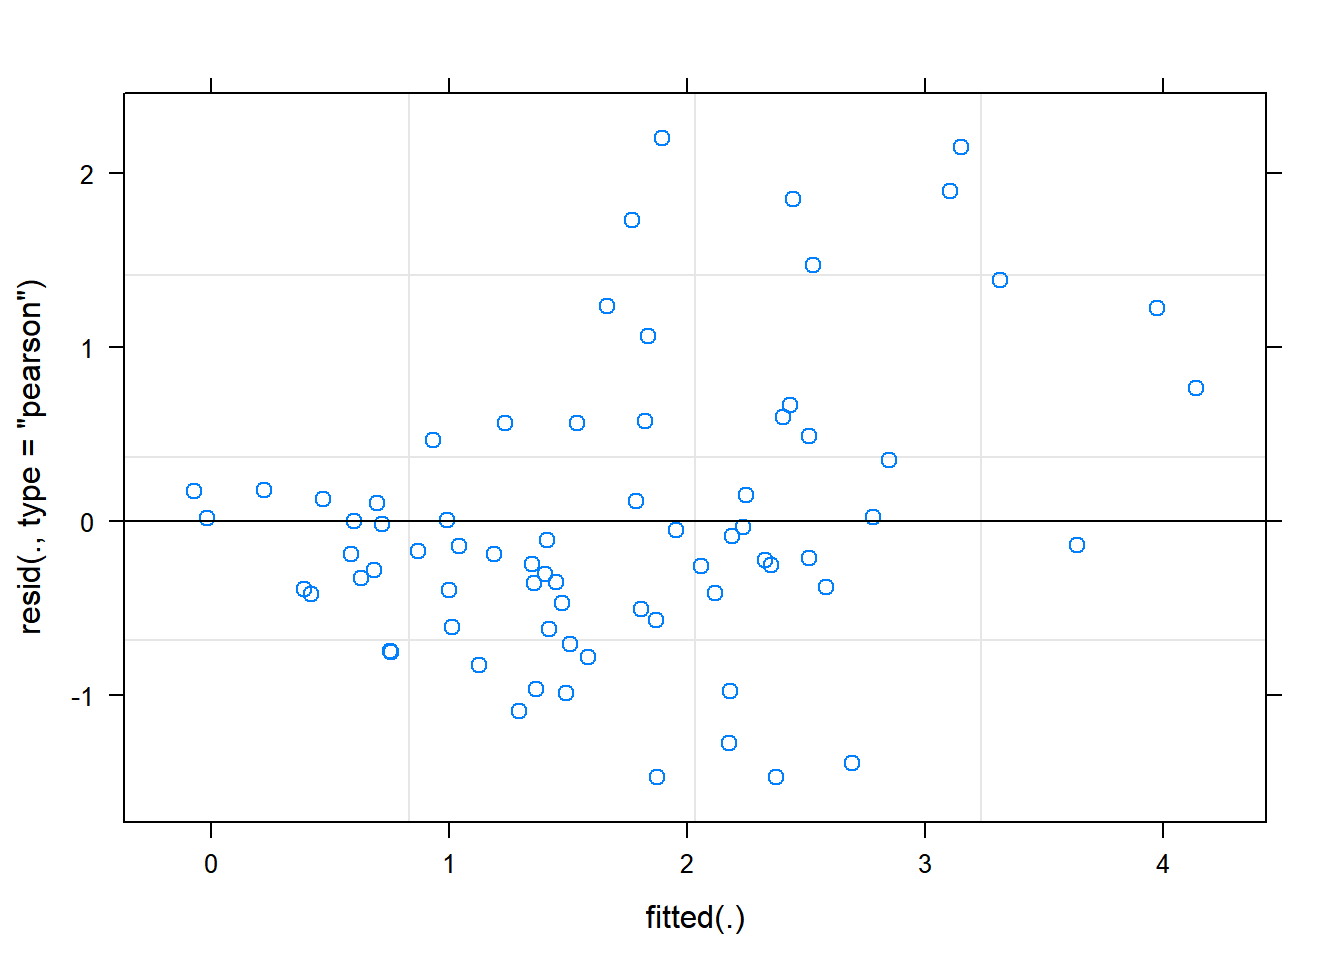
\includegraphics{bookdown-demo_files/figure-latex/unnamed-chunk-57-1.pdf}
The residual Vs fitted plot is a scatter plot of the Residuals on the
y-axis and the fitted on the x-axis and the aim for this plot is to test
the assumption of equal variance of the residuals across the range of
fitted values. There is someevidence of non-constant variance in our
plot - residual values are less varaable around lower fitted values, and
more variable around higher fitted values. This issue can often be
solved by using a logaithmic or square root transformation. In this
case, because there are some zero values within our data, it may be
better to use a square root transformation.

\begin{Shaded}
\begin{Highlighting}[]
\NormalTok{splitplotmodel2<-}\KeywordTok{lmer}\NormalTok{(}\KeywordTok{sqrt}\NormalTok{(grain)}\OperatorTok{~}\NormalTok{fallow}\OperatorTok{*}\NormalTok{nitrogen}\OperatorTok{+}\NormalTok{(}\DecValTok{1}\OperatorTok{|}\NormalTok{block}\OperatorTok{/}\NormalTok{mainplot), }\DataTypeTok{data=}\NormalTok{fphosphorus)}
\end{Highlighting}
\end{Shaded}

Refitting the plot shows a better approximation of heterogeneity, that
is more acceptable to the assumptions required.

\begin{Shaded}
\begin{Highlighting}[]
\KeywordTok{plot}\NormalTok{(splitplotmodel2)}
\end{Highlighting}
\end{Shaded}

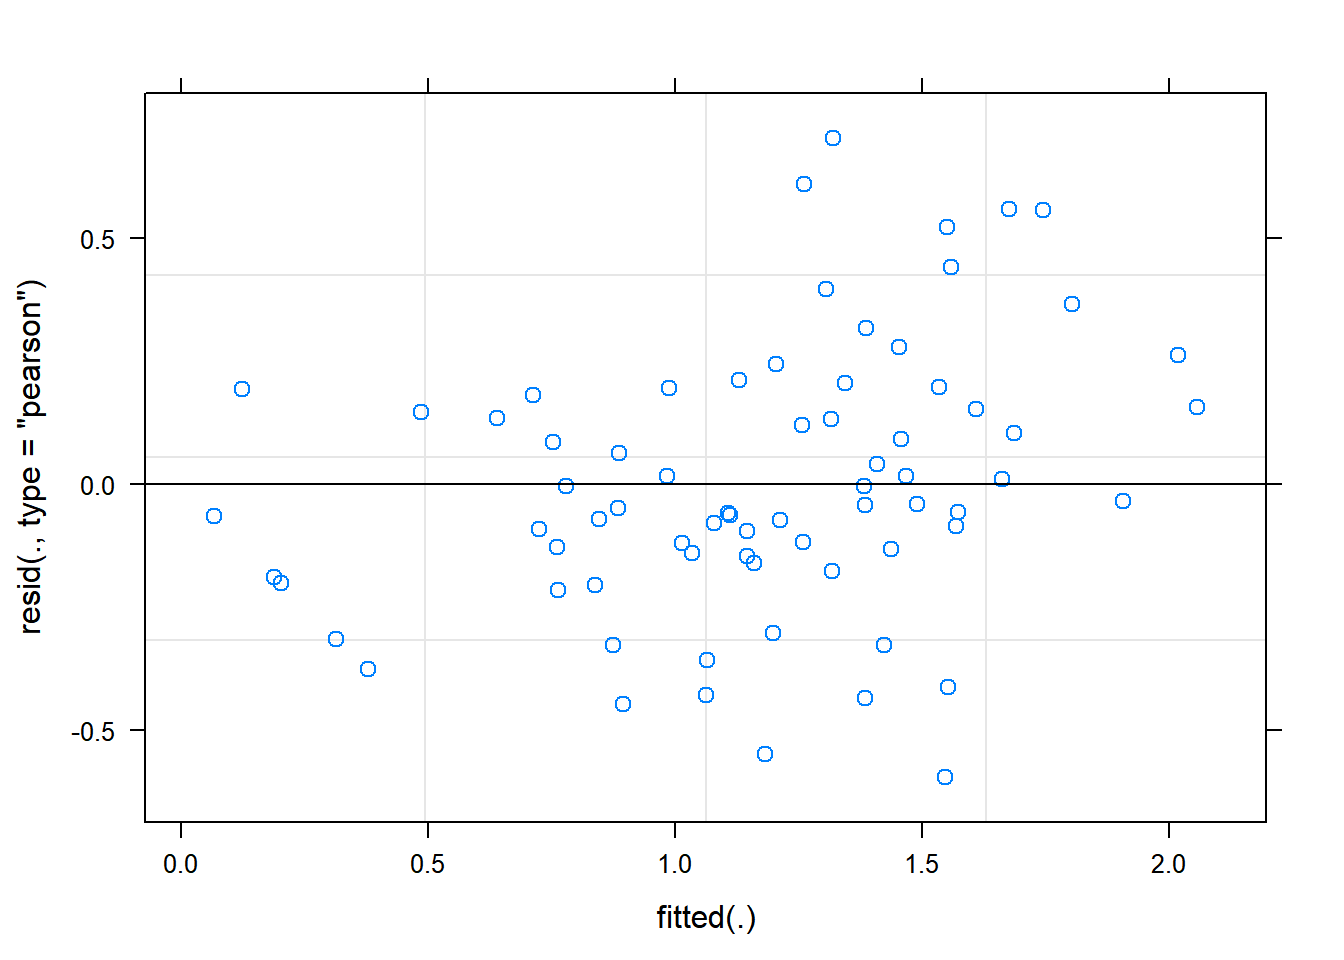
\includegraphics{bookdown-demo_files/figure-latex/unnamed-chunk-59-1.pdf}
We can also see that there are no extreme values in the residuals which
might be potentially causing problems with the validity of our
conclusions (leverage)

To assess the assumption of normality we can produce a qqplot. This
shows us how closely the residuals follow a normal distribution - if
there are severe and syste,matic deviations from the line then we may
want to consider an alternative distribution.

\begin{Shaded}
\begin{Highlighting}[]
\KeywordTok{qqnorm}\NormalTok{(}\KeywordTok{resid}\NormalTok{(splitplotmodel2))}
\KeywordTok{qqline}\NormalTok{(}\KeywordTok{resid}\NormalTok{(splitplotmodel2))}
\end{Highlighting}
\end{Shaded}

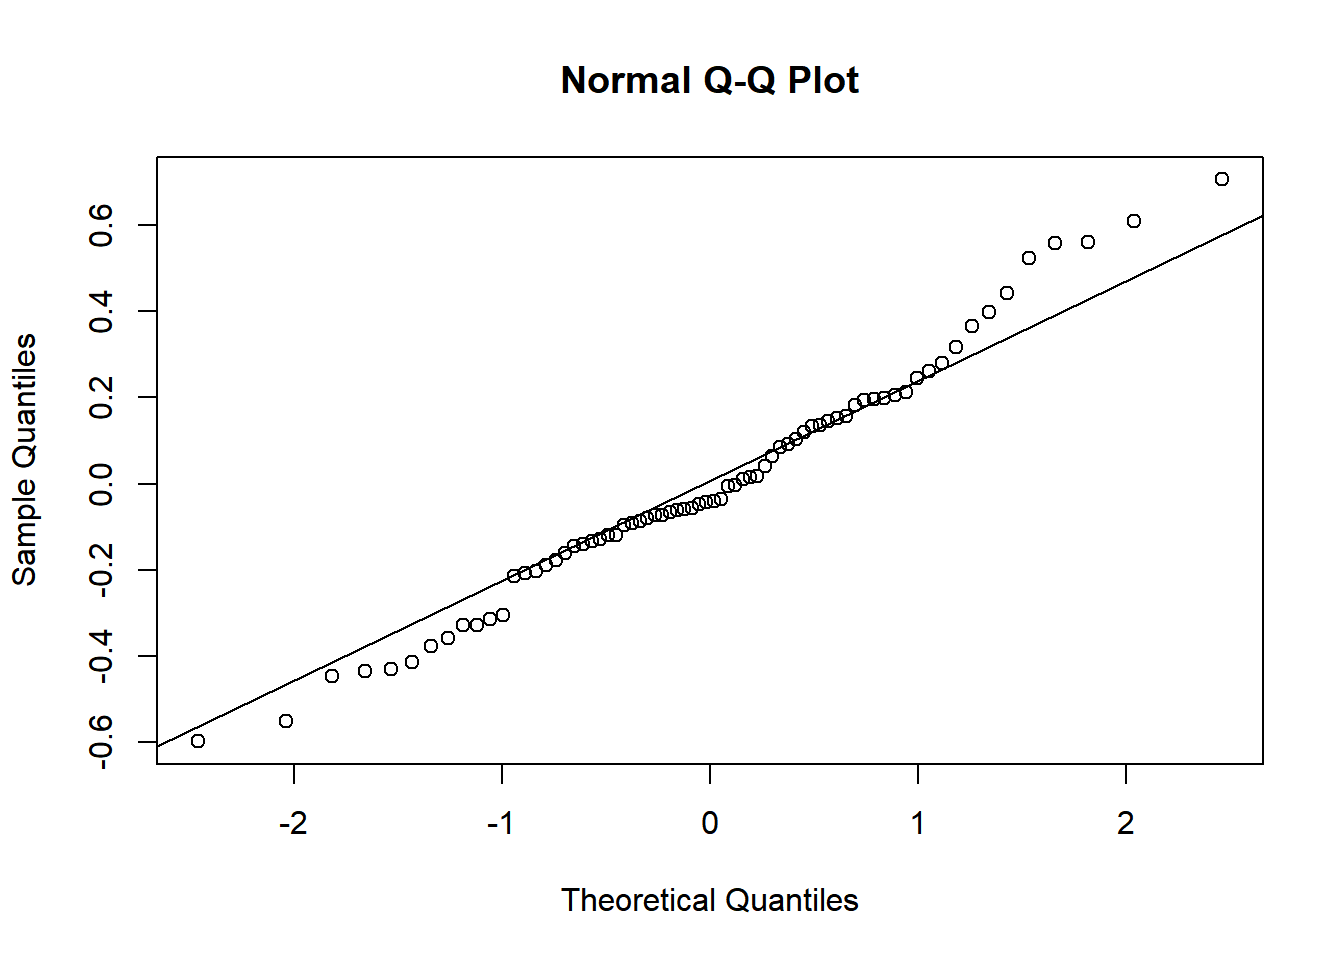
\includegraphics{bookdown-demo_files/figure-latex/unnamed-chunk-60-1.pdf}
In this case the residuals seem to fit the assumption required for
normality.

\subsection{7. Interpret Model}\label{interpret-model-1}

The anova() function only prints the rows of analysis of variance table
for treatment effects when looking at a mixed model fitted using lmer().

\begin{Shaded}
\begin{Highlighting}[]
\KeywordTok{anova}\NormalTok{(splitplotmodel2,}\DataTypeTok{ddf=}\StringTok{"Kenward-Roger"}\NormalTok{)}
\end{Highlighting}
\end{Shaded}

\begin{verbatim}
## Type III Analysis of Variance Table with Kenward-Roger's method
##                  Sum Sq Mean Sq NumDF DenDF F value Pr(>F)
## fallow          0.38006 0.12669     3    24  1.0112 0.4050
## nitrogen        0.27129 0.27129     1    32  2.1653 0.1509
## fallow:nitrogen 0.37536 0.12512     3    32  0.9987 0.4061
\end{verbatim}

ddf=Kenward-Roger tells R which method to use for determining the
calculations of the table; this option matches the defaults found within
SAS or Genstat. The ANOVA table suggests a highly significant effect of
the treatment on the yield.

To obtain the residual variance, and the variance attributed to the
blocks we need an additional command. From these number it is possible
to reconstruct a more classic ANOVA table, if so desired.

\begin{Shaded}
\begin{Highlighting}[]
\KeywordTok{print}\NormalTok{(}\KeywordTok{VarCorr}\NormalTok{(splitplotmodel1), }\DataTypeTok{comp=}\NormalTok{(}\StringTok{"Variance"}\NormalTok{))}
\end{Highlighting}
\end{Shaded}

\begin{verbatim}
##  Groups         Name        Variance
##  mainplot:block (Intercept) 0.38238 
##  block          (Intercept) 0.64581 
##  Residual                   1.04375
\end{verbatim}

\subsection{8. Present the results from the
model}\label{present-the-results-from-the-model-1}

To help understand what the significant result from the ANOVA table
means we can produce several plots and tables to help us. First we can
use the function emmip() to produce plots of the modelled results,
including 95\% confidence intervals.

\begin{Shaded}
\begin{Highlighting}[]
\KeywordTok{emmip}\NormalTok{(splitplotmodel2,nitrogen}\OperatorTok{~}\NormalTok{fallow,}\DataTypeTok{CIs =} \OtherTok{TRUE}\NormalTok{,}\DataTypeTok{type =} \StringTok{"response"}\NormalTok{)}
\end{Highlighting}
\end{Shaded}

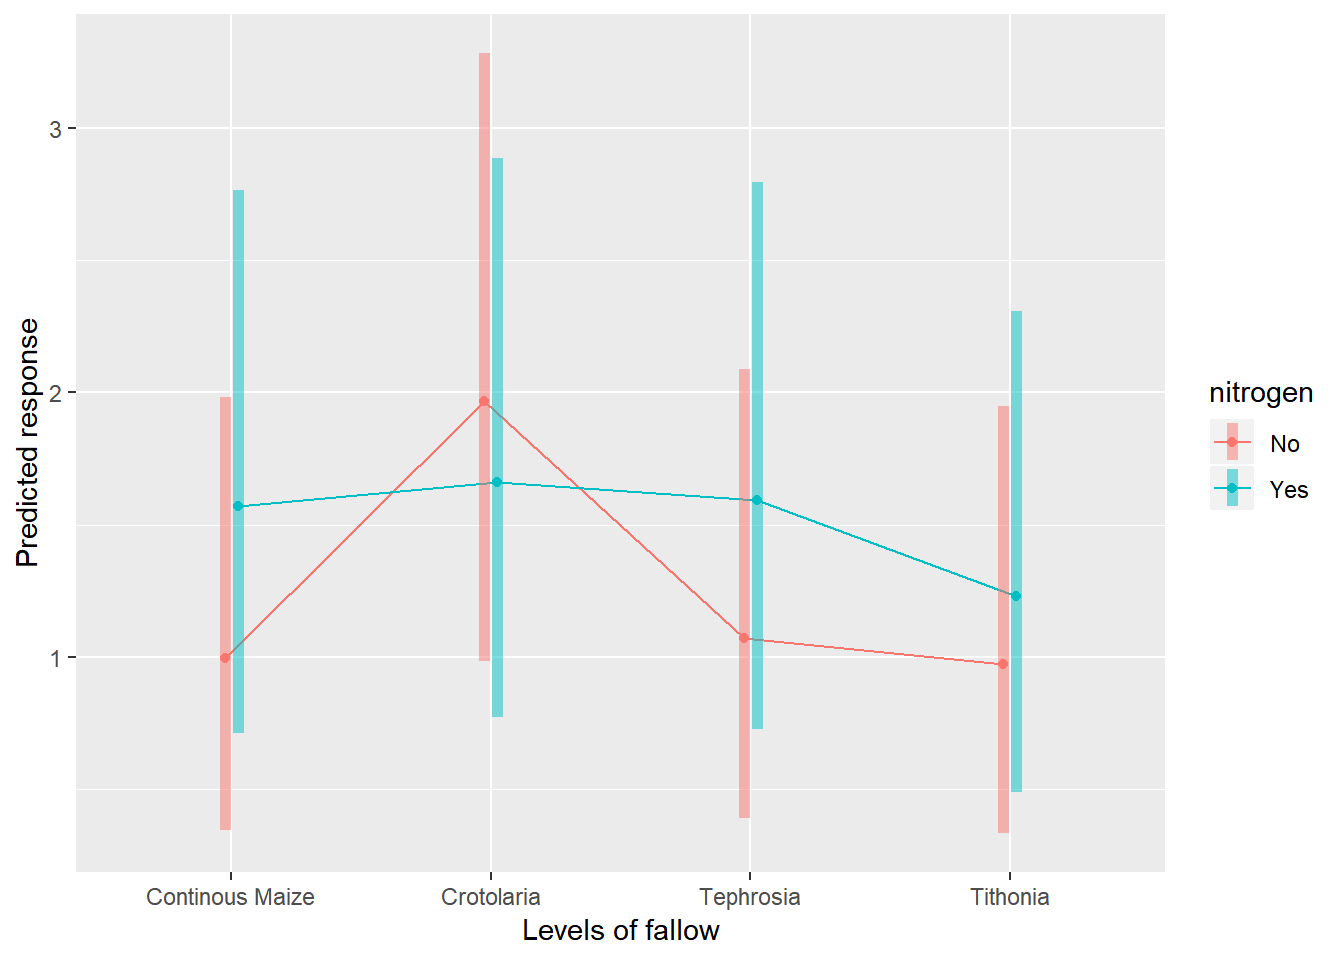
\includegraphics{bookdown-demo_files/figure-latex/unnamed-chunk-63-1.pdf}

To obtain the numbers used in creating this graph we can use the
function emmeans.

\begin{Shaded}
\begin{Highlighting}[]
\KeywordTok{emmeans}\NormalTok{(splitplotmodel1, }\OperatorTok{~}\NormalTok{fallow)}
\end{Highlighting}
\end{Shaded}

\begin{verbatim}
## NOTE: Results may be misleading due to involvement in interactions
\end{verbatim}

\begin{verbatim}
##  fallow            emmean       SE    df  lower.CL upper.CL
##  Continous Maize 1.688889 0.415006 21.04 0.8259423 2.551835
##  Crotolaria      2.155556 0.415006 21.04 1.2926090 3.018502
##  Tephrosia       1.494444 0.415006 21.04 0.6314978 2.357391
##  Tithonia        1.461111 0.415006 21.04 0.5981645 2.324058
## 
## Results are averaged over the levels of: nitrogen 
## Degrees-of-freedom method: kenward-roger 
## Confidence level used: 0.95
\end{verbatim}

And one method for conducting mean separation analysis we can use the
function cld().

\begin{Shaded}
\begin{Highlighting}[]
\KeywordTok{cld}\NormalTok{(}\KeywordTok{emmeans}\NormalTok{(splitplotmodel1, }\OperatorTok{~}\NormalTok{fallow))}
\end{Highlighting}
\end{Shaded}

\begin{verbatim}
## NOTE: Results may be misleading due to involvement in interactions
\end{verbatim}

\begin{verbatim}
##  fallow            emmean       SE    df  lower.CL upper.CL .group
##  Tithonia        1.461111 0.415006 21.04 0.5981645 2.324058  1    
##  Tephrosia       1.494444 0.415006 21.04 0.6314978 2.357391  1    
##  Continous Maize 1.688889 0.415006 21.04 0.8259423 2.551835  1    
##  Crotolaria      2.155556 0.415006 21.04 1.2926090 3.018502  1    
## 
## Results are averaged over the levels of: nitrogen 
## Degrees-of-freedom method: kenward-roger 
## Confidence level used: 0.95 
## P value adjustment: tukey method for comparing a family of 4 estimates 
## significance level used: alpha = 0.05
\end{verbatim}

In the output, groups sharing a letter in the .group are not
statistically different from each other.

\section{Section 3 -- Methodological
Principles}\label{section-3-methodological-principles-1}

There are always many different ways of doing all that we have done here
in R. The less complex the method/code is, the better it is for you so
that you can easily grasp the method.

In this example using the phosphurus data, we have a split plot design.
This means that a single plot where the fallow treatment has been
applied is split into 2, and each half receives a different nitrogen
treatment. It is useful to have seperate columns denoting treamtent
factors and layout factors - even if these may be somewhat replicating
the same information. The split plots are nested within the plots, which
are nested within the blocks. So the random effect needs to incorporate
this nesting. Remember that the lowest level design factor, the split
plot, does not get included in the model. This is similar to the RCBD
analysis, where the lowest level factor - plot, does not get included in
the model.

Note that the difference in the specification of random effects in the
model is effectively the only difference needed in the R syntax used to
produce this analysis, as compared to Tutorial 1, the RCBD. All other
syntax has been modified to reflect differences in the data collected,
but the same functions (ggplot, summaryBy, emmeans) are being applied in
the same way.

Food for thought: Your best model will certainly be as good as the data
you collected!!!

\chapter{Adjusting for Covariates}\label{adjusting-for-covariates}

\section{About the data}\label{about-the-data-2}

The data used in this example is from a study was conducted in Eastern
Zambia and the main aim was to improve on the efficiency of the natural
fallows by using appropriate trees that may have relevance in soil
fertility regeneration within permissible fallow periods. This is the
same data used in the first part of this series.

The design was a randomized complete block design experiment with 4
blocks and 9 treatments was conducted. The primary outcome variable was
crop yield (yield). We also have data collected on striga infestation.

The objective for this analysis is to investigate the relationship
between striga infestation and yield across the different treatments.

The following steps were followed to generate the output in this
document. The data was organized in excel rectangle columns with the
different variables appearing in excel columns. All data checks were
done in excel, meaningful data was selected and a copy of this data file
was stored as a CSV file to make data import easy in R. The data file
used in this analysis can be downloaded here:
\url{https://bit.ly/2rfLBEt}

\section{Section 1: Steps in analysis using
R}\label{section-1-steps-in-analysis-using-r-2}

\begin{enumerate}
\def\labelenumi{\arabic{enumi}.}
\tightlist
\item
  Install R packages needed
\end{enumerate}

\begin{Shaded}
\begin{Highlighting}[]
\KeywordTok{library}\NormalTok{(ggplot2)}
\KeywordTok{library}\NormalTok{(emmeans)}
\KeywordTok{library}\NormalTok{(doBy)}
\KeywordTok{library}\NormalTok{(lmerTest)}
\KeywordTok{library}\NormalTok{(multcompView)}
\end{Highlighting}
\end{Shaded}

\begin{enumerate}
\def\labelenumi{\arabic{enumi}.}
\setcounter{enumi}{1}
\tightlist
\item
  Import data
\end{enumerate}

\begin{Shaded}
\begin{Highlighting}[]
\NormalTok{fallow <-}\StringTok{ }\KeywordTok{read.csv}\NormalTok{(}\StringTok{"C:/Users/Admin/Desktop/Fallow N2.csv"}\NormalTok{)}
\end{Highlighting}
\end{Shaded}

\begin{enumerate}
\def\labelenumi{\arabic{enumi}.}
\setcounter{enumi}{2}
\tightlist
\item
  Check and update data
\end{enumerate}

\begin{Shaded}
\begin{Highlighting}[]
\KeywordTok{summary}\NormalTok{(fallow)}
\KeywordTok{str}\NormalTok{(fallow)}
\NormalTok{fallow}\OperatorTok{$}\NormalTok{rep<-}\KeywordTok{factor}\NormalTok{(fallow}\OperatorTok{$}\NormalTok{rep)}
\NormalTok{fallow}\OperatorTok{$}\NormalTok{plot<-}\KeywordTok{factor}\NormalTok{(fallow}\OperatorTok{$}\NormalTok{plot)}
\end{Highlighting}
\end{Shaded}

\begin{enumerate}
\def\labelenumi{\arabic{enumi}.}
\setcounter{enumi}{3}
\tightlist
\item
  Explore data
\end{enumerate}

\begin{Shaded}
\begin{Highlighting}[]
\KeywordTok{ggplot}\NormalTok{(}\DataTypeTok{data=}\NormalTok{fallow,}\KeywordTok{aes}\NormalTok{(}\DataTypeTok{y=}\NormalTok{yield,}\DataTypeTok{x=}\NormalTok{treat,}\DataTypeTok{col=}\NormalTok{rep))}\OperatorTok{+}\KeywordTok{geom_point}\NormalTok{()}
\KeywordTok{summaryBy}\NormalTok{(yield}\OperatorTok{~}\NormalTok{treat, }\DataTypeTok{data=}\NormalTok{fallow, }\DataTypeTok{FUN=}\KeywordTok{c}\NormalTok{(min,max,mean,median,sd))}
\end{Highlighting}
\end{Shaded}

\begin{enumerate}
\def\labelenumi{\arabic{enumi}.}
\setcounter{enumi}{4}
\tightlist
\item
  Specify a model for data
\end{enumerate}

\begin{Shaded}
\begin{Highlighting}[]
\NormalTok{rcbdmodel1<-}\KeywordTok{lmer}\NormalTok{(yield}\OperatorTok{~}\NormalTok{treat}\OperatorTok{+}\NormalTok{(}\DecValTok{1}\OperatorTok{|}\NormalTok{rep),}\DataTypeTok{data=}\NormalTok{fallow)}
\end{Highlighting}
\end{Shaded}

\begin{enumerate}
\def\labelenumi{\arabic{enumi}.}
\setcounter{enumi}{5}
\tightlist
\item
  Check the model
\end{enumerate}

\begin{Shaded}
\begin{Highlighting}[]
\KeywordTok{plot}\NormalTok{(rcbdmodel1)}

\KeywordTok{qqnorm}\NormalTok{(}\KeywordTok{resid}\NormalTok{(rcbdmodel1))}
\KeywordTok{qqline}\NormalTok{(}\KeywordTok{resid}\NormalTok{(rcbdmodel1))}
\end{Highlighting}
\end{Shaded}

\begin{enumerate}
\def\labelenumi{\arabic{enumi}.}
\setcounter{enumi}{6}
\tightlist
\item
  Interpret the model
\end{enumerate}

\begin{Shaded}
\begin{Highlighting}[]
\KeywordTok{anova}\NormalTok{(rcbdmodel1,}\DataTypeTok{ddf=}\StringTok{"Kenward-Roger"}\NormalTok{)}
\KeywordTok{print}\NormalTok{(}\KeywordTok{VarCorr}\NormalTok{(rcbdmodel1), }\DataTypeTok{comp=}\NormalTok{(}\StringTok{"Variance"}\NormalTok{))}
\end{Highlighting}
\end{Shaded}

\begin{enumerate}
\def\labelenumi{\arabic{enumi}.}
\setcounter{enumi}{7}
\tightlist
\item
  Present the results from the model
\end{enumerate}

\begin{Shaded}
\begin{Highlighting}[]
\KeywordTok{emmip}\NormalTok{(rcbdmodel1,}\OperatorTok{~}\NormalTok{treat,}\DataTypeTok{CIs =} \OtherTok{TRUE}\NormalTok{)}
\KeywordTok{emmeans}\NormalTok{(rcbdmodel1, }\OperatorTok{~}\NormalTok{treat)}
\KeywordTok{cld}\NormalTok{(}\KeywordTok{emmeans}\NormalTok{(rcbdmodel1, }\OperatorTok{~}\NormalTok{treat))}
\end{Highlighting}
\end{Shaded}

\section{Section 2: Explanation of
Steps}\label{section-2-explanation-of-steps-2}

\subsection{1. Install R packages
needed}\label{install-r-packages-needed-2}

A number of packages following packages were used during data
exploration and analysis. For a general introduction explaining what R
packages are and how they work, this is a really useful guide
\url{https://www.datacamp.com/community/tutorials/r-packages-guide}. For
each of these packages to be installed, using install.packages(), this
requires a reliable internet connection and a correctly installed
version of R and RStudio. If you are having difficulties installing
these packages please ask for help.

\begin{Shaded}
\begin{Highlighting}[]
\KeywordTok{install.packages}\NormalTok{(}\StringTok{"ggplot2"}\NormalTok{)}
\KeywordTok{library}\NormalTok{(ggplot2)}
\end{Highlighting}
\end{Shaded}

\texttt{ggplot2} This package provides a powerful graphics language for
creating elegant and complex graphs in R.

\begin{Shaded}
\begin{Highlighting}[]
\KeywordTok{install.packages}\NormalTok{(}\StringTok{"emmeans"}\NormalTok{)}
\KeywordTok{library}\NormalTok{(emmeans)}
\end{Highlighting}
\end{Shaded}

\texttt{emmeans} Estimated marginal means (also known as least squares
means) helps provide expected mean values and confidence intervals from
statistical models.

\begin{Shaded}
\begin{Highlighting}[]
\KeywordTok{install.packages}\NormalTok{(}\StringTok{"doBy"}\NormalTok{)}
\KeywordTok{library}\NormalTok{(doBy)}
\end{Highlighting}
\end{Shaded}

\texttt{doBy}Allows easy production of summary statistic tables

\begin{Shaded}
\begin{Highlighting}[]
\KeywordTok{install.packages}\NormalTok{(}\StringTok{"lmerTest"}\NormalTok{)}
\KeywordTok{library}\NormalTok{(lmerTest)}
\end{Highlighting}
\end{Shaded}

\texttt{lmerTest} Allows produce of flexible mixed effects regression
models, similar to REML in Genstat.

\begin{Shaded}
\begin{Highlighting}[]
\KeywordTok{install.packages}\NormalTok{(}\StringTok{"multcompView"}\NormalTok{)}
\KeywordTok{library}\NormalTok{(multcompView)}
\end{Highlighting}
\end{Shaded}

\texttt{multcompView} allows for mean seperation methods on analyses

\subsection{2. Import data}\label{import-data-2}

Our data set saved as a CSV file, so we can use the read.csv commmand to
import the data. We are going to assign the name of the data with R to
be \texttt{fallow2}. Remember in R Studio you could also use the
``Import Dataset'' menu to import a dataset.

\begin{Shaded}
\begin{Highlighting}[]
\NormalTok{fallow <-}\StringTok{ }\KeywordTok{read.csv}\NormalTok{(}\StringTok{"C:/Users/Admin/Desktop/Fallow N2.csv"}\NormalTok{)}
\end{Highlighting}
\end{Shaded}

\subsection{3. Check and update data}\label{check-and-update-data-2}

When reading data into R it is always useful to check that data is in
the format expected. How many variables are there? How many rows? How
have the columns been read in? The summary command can help to show if
the data is being treated correctly.

\begin{Shaded}
\begin{Highlighting}[]
\KeywordTok{summary}\NormalTok{(fallow)}
\end{Highlighting}
\end{Shaded}

\begin{verbatim}
##       rep            plot            treat        yield      
##  Min.   :1.00   Min.   :1   1 S.sesban  : 4   Min.   :1.140  
##  1st Qu.:1.75   1st Qu.:3   2 G.sepium  : 4   1st Qu.:2.370  
##  Median :2.50   Median :5   3 L.leuco   : 4   Median :3.140  
##  Mean   :2.50   Mean   :5   4 F.congesta: 4   Mean   :3.232  
##  3rd Qu.:3.25   3rd Qu.:7   5 C.siamea  : 4   3rd Qu.:3.728  
##  Max.   :4.00   Max.   :9   6 C.calo    : 4   Max.   :6.540  
##                             (Other)     :12                  
##      striga      
##  Min.   :   0.0  
##  1st Qu.:   0.0  
##  Median :  21.0  
##  Mean   : 334.1  
##  3rd Qu.: 238.5  
##  Max.   :2798.0  
## 
\end{verbatim}

Where data is being treated as a numeric variable (i.e.~a number)
\texttt{summary} provides statistics like the mean, min and max. Where
data is being treated like a categorical variable (i.e.~a group) then
summary provides frequency tables.

From the results we can see that the variables rep and plot are being
considered as numeric variables. However these are grouping variables,
not number variables, the numbers used are simply codes. If we do not
rectify this then our analysis later will be incorrect and
meaningless.\\
This can also be seen more explicitly using the str() function.

\begin{Shaded}
\begin{Highlighting}[]
\KeywordTok{str}\NormalTok{(fallow)}
\end{Highlighting}
\end{Shaded}

\begin{verbatim}
## 'data.frame':    36 obs. of  5 variables:
##  $ rep   : int  1 4 4 1 1 3 3 1 3 2 ...
##  $ plot  : int  2 3 6 9 7 3 8 6 9 9 ...
##  $ treat : Factor w/ 9 levels "1 S.sesban","2 G.sepium",..: 8 5 8 7 5 8 5 9 6 5 ...
##  $ yield : num  1.14 1.74 1.95 2.06 2.09 2.15 2.21 2.22 2.34 2.38 ...
##  $ striga: int  2798 0 1787 129 1 1144 0 228 0 0 ...
\end{verbatim}

So we need to convert these variables into factors.

\begin{Shaded}
\begin{Highlighting}[]
\NormalTok{fallow}\OperatorTok{$}\NormalTok{rep<-}\KeywordTok{factor}\NormalTok{(fallow}\OperatorTok{$}\NormalTok{rep)}
\NormalTok{fallow}\OperatorTok{$}\NormalTok{plot<-}\KeywordTok{factor}\NormalTok{(fallow}\OperatorTok{$}\NormalTok{plot)}
\end{Highlighting}
\end{Shaded}

These commands take the column rep within the data frame fallow,
converts into a factor and saves the result in a column called rep
within fallow.

\subsection{4. Explore data}\label{explore-data-2}

\subsubsection{Plots}\label{plots-2}

We are now interesting in assessing the relationship between yield and
striga - so we want to produce a plot of striga against yield, with
different coloured points denoting each treatment.

\begin{Shaded}
\begin{Highlighting}[]
\KeywordTok{ggplot}\NormalTok{(}\DataTypeTok{data=}\NormalTok{fallow,}\KeywordTok{aes}\NormalTok{(}\DataTypeTok{y=}\NormalTok{yield,}\DataTypeTok{x=}\NormalTok{striga,}\DataTypeTok{col=}\NormalTok{treat))}\OperatorTok{+}\KeywordTok{geom_point}\NormalTok{()}
\end{Highlighting}
\end{Shaded}

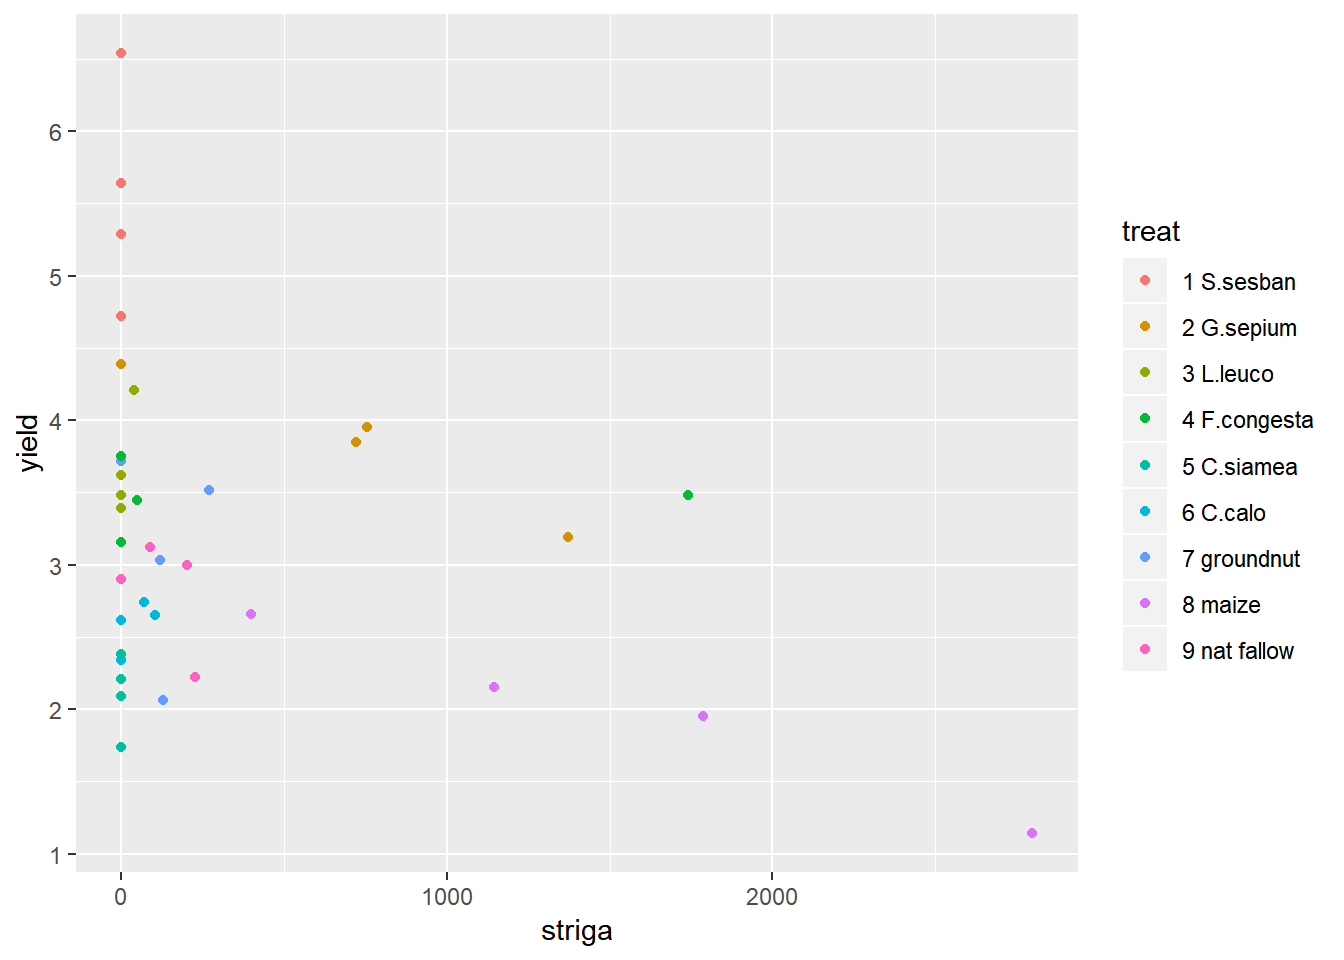
\includegraphics{bookdown-demo_files/figure-latex/unnamed-chunk-85-1.pdf}
We can see from the distribution of striga that there are some farms
with very high levels of striga, and some farms with no striga. The big
range of values makes it hard to make interpretations from this plot, so
taking a square root transformation may help to visualise the
relationship. A log transformation will not help here because of the
large number of 0 values of striga.

\begin{Shaded}
\begin{Highlighting}[]
\KeywordTok{ggplot}\NormalTok{(}\DataTypeTok{data=}\NormalTok{fallow,}\KeywordTok{aes}\NormalTok{(}\DataTypeTok{y=}\NormalTok{yield,}\DataTypeTok{x=}\KeywordTok{sqrt}\NormalTok{(striga),}\DataTypeTok{col=}\NormalTok{treat))}\OperatorTok{+}\KeywordTok{geom_point}\NormalTok{()}
\end{Highlighting}
\end{Shaded}

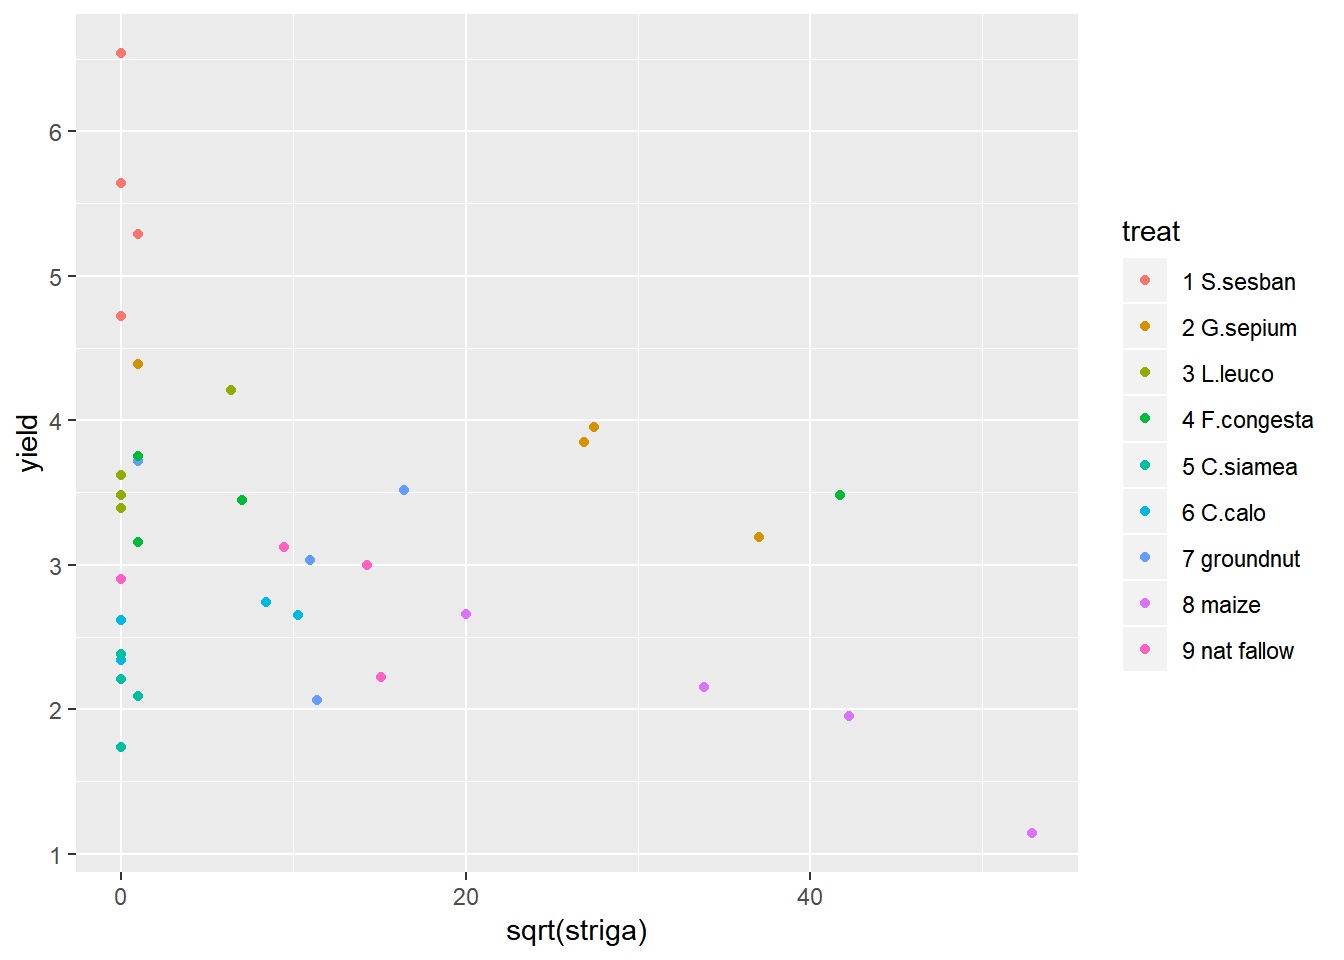
\includegraphics{bookdown-demo_files/figure-latex/unnamed-chunk-86-1.pdf}

\begin{Shaded}
\begin{Highlighting}[]
\KeywordTok{ggplot}\NormalTok{(}\DataTypeTok{data=}\NormalTok{fallow,}\KeywordTok{aes}\NormalTok{(}\DataTypeTok{y=}\NormalTok{yield,}\DataTypeTok{x=}\KeywordTok{sqrt}\NormalTok{(striga)))}\OperatorTok{+}\KeywordTok{geom_point}\NormalTok{(}\KeywordTok{aes}\NormalTok{(}\DataTypeTok{col=}\NormalTok{treat))}\OperatorTok{+}\KeywordTok{geom_smooth}\NormalTok{(}\DataTypeTok{method=}\StringTok{"lm"}\NormalTok{)}
\end{Highlighting}
\end{Shaded}

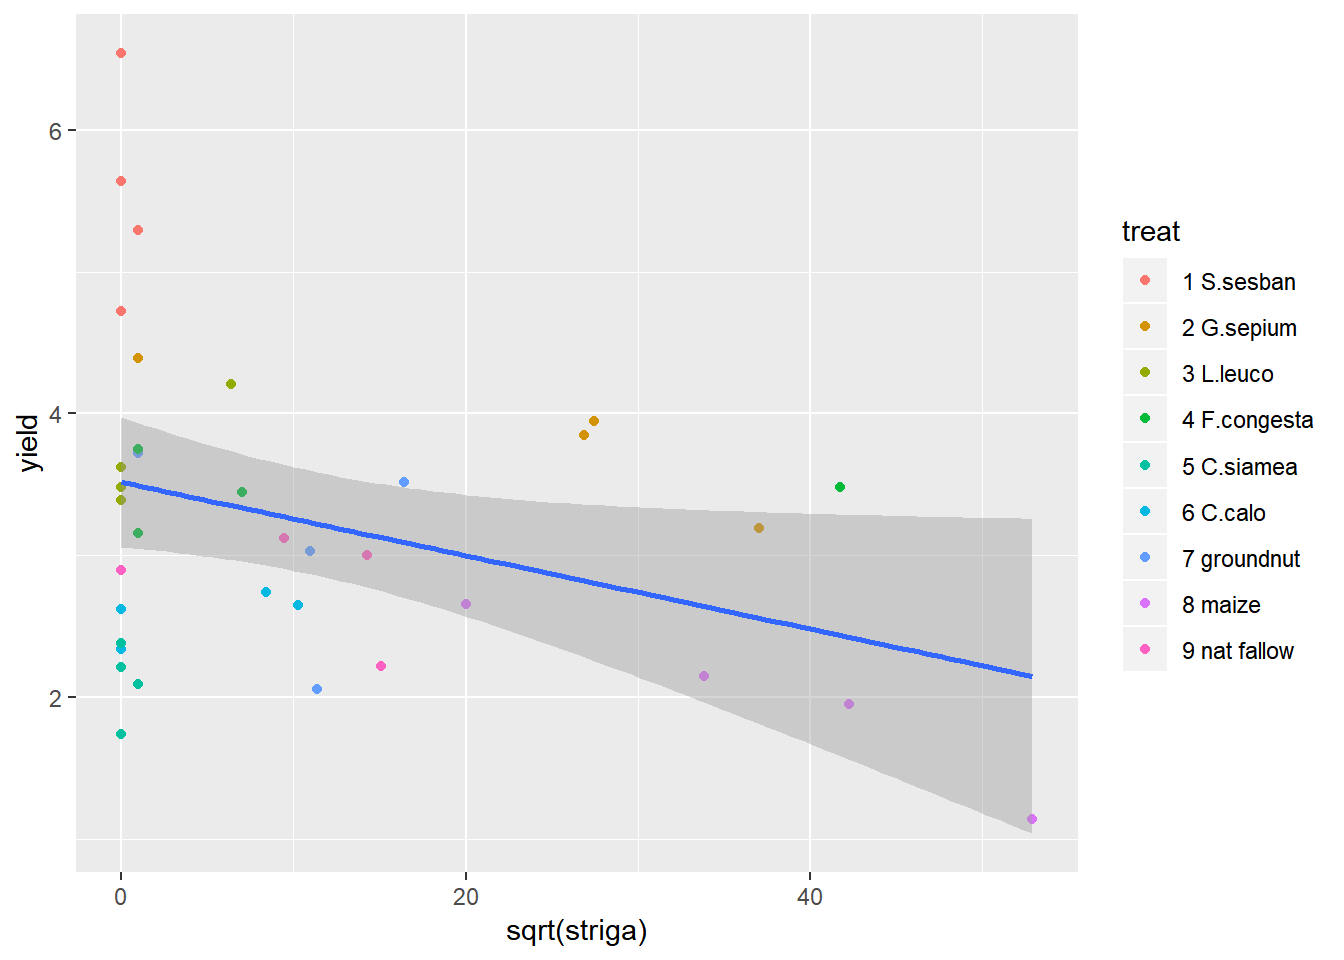
\includegraphics{bookdown-demo_files/figure-latex/unnamed-chunk-87-1.pdf}
\#\#\#\#Summary Statistics

To produce summary statistics, by group, there are many options within
R. One option is to use the summaryBy function, from the doBy library.
The code used for this is quite similar to the code we will use to
produce models in a later step.

\begin{Shaded}
\begin{Highlighting}[]
\KeywordTok{summaryBy}\NormalTok{(yield}\OperatorTok{~}\NormalTok{treat, }\DataTypeTok{data=}\NormalTok{fallow, }\DataTypeTok{FUN=}\NormalTok{mean)}
\end{Highlighting}
\end{Shaded}

\begin{verbatim}
##          treat yield.mean
## 1   1 S.sesban     5.5475
## 2   2 G.sepium     3.8450
## 3    3 L.leuco     3.6750
## 4 4 F.congesta     3.4600
## 5   5 C.siamea     2.1050
## 6     6 C.calo     2.5875
## 7  7 groundnut     3.0825
## 8      8 maize     1.9750
## 9 9 nat fallow     2.8100
\end{verbatim}

We can also calculate multiple statistics in the same line of code

\begin{Shaded}
\begin{Highlighting}[]
\KeywordTok{summaryBy}\NormalTok{(yield}\OperatorTok{+}\NormalTok{striga}\OperatorTok{~}\NormalTok{treat, }\DataTypeTok{data=}\NormalTok{fallow, }\DataTypeTok{FUN=}\KeywordTok{c}\NormalTok{(mean,median,sd))}
\end{Highlighting}
\end{Shaded}

\begin{verbatim}
##          treat yield.mean striga.mean yield.median striga.median  yield.sd
## 1   1 S.sesban     5.5475        0.25        5.465           0.0 0.7625997
## 2   2 G.sepium     3.8450      712.00        3.900         738.0 0.4956813
## 3    3 L.leuco     3.6750       10.25        3.550           0.0 0.3690077
## 4 4 F.congesta     3.4600      448.00        3.465          25.0 0.2412468
## 5   5 C.siamea     2.1050        0.25        2.150           0.0 0.2708628
## 6     6 C.calo     2.5875       44.00        2.635          35.5 0.1726992
## 7  7 groundnut     3.0825      130.00        3.275         124.5 0.7407372
## 8      8 maize     1.9750     1532.25        2.050        1465.5 0.6318491
## 9 9 nat fallow     2.8100      130.00        2.950         146.0 0.4034848
##    striga.sd
## 1    0.50000
## 2  560.27731
## 3   20.50000
## 4  862.29693
## 5    0.50000
## 6   52.66878
## 7  110.06362
## 8 1016.48885
## 9  105.69453
\end{verbatim}

\subsection{5. Specify a model for
data}\label{specify-a-model-for-data-2}

In this design, an RCBD, we have one treatment factor, ``treat'', and
one layout factor ``rep''. More information about model fitting can be
found in section 2.

\begin{Shaded}
\begin{Highlighting}[]
\NormalTok{rcbdmodel2<-}\KeywordTok{lmer}\NormalTok{(yield}\OperatorTok{~}\NormalTok{treat}\OperatorTok{+}\KeywordTok{sqrt}\NormalTok{(striga)}\OperatorTok{+}\NormalTok{(}\DecValTok{1}\OperatorTok{|}\NormalTok{rep),}\DataTypeTok{data=}\NormalTok{fallow)}
\end{Highlighting}
\end{Shaded}

R is unlike many other software packages in how it fits models. The best
way of handling models in R is to assign the model to a name (in this
case rcbdmodel1) and then ask R to provide different sorts of output for
this model. When you run the above line you will get now output from the
data - this is what we expected to see!

\subsection{6. Check the model}\label{check-the-model-2}

Before interpretting the model any further we should investigate the
model validity, to ensure any conclusions we draw are valid. There are 3
assumptions that we can check for using standard model checking plots.
1. Homogeneity (equal variance) 2. Values with high leverage 3.
Normality of residuals

The function plot() when used with a model will plot the fitted values
from the model against the expected values.

\begin{Shaded}
\begin{Highlighting}[]
\KeywordTok{plot}\NormalTok{(rcbdmodel2)}
\end{Highlighting}
\end{Shaded}

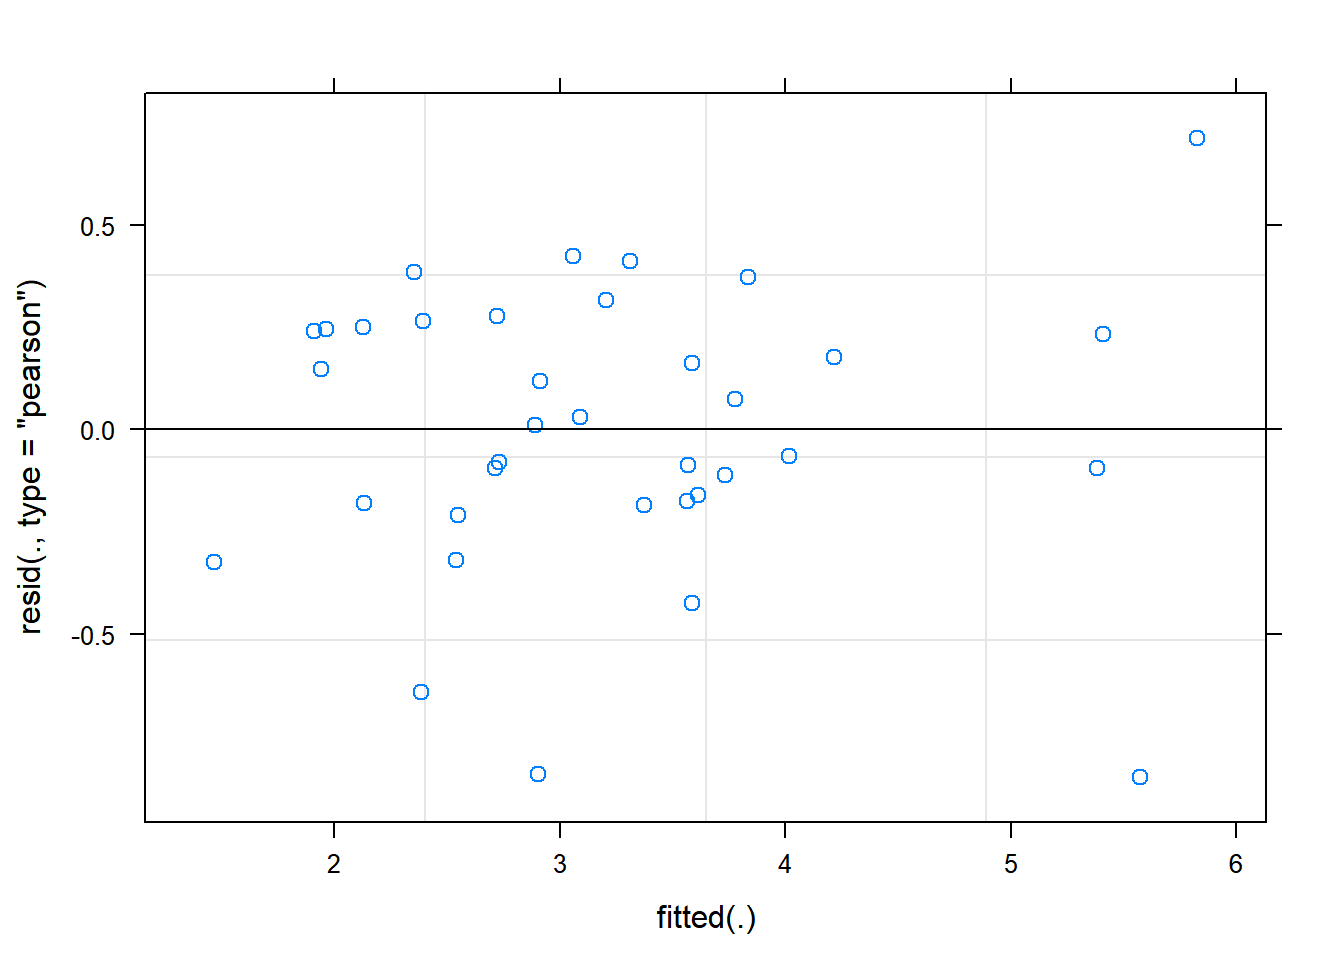
\includegraphics{bookdown-demo_files/figure-latex/unnamed-chunk-91-1.pdf}
The residual Vs fitted plot is a scatter plot of the Residuals on the
y-axis and the fitted on the x-axis and the aim for this plot is to test
the assumption of equal variance of the residuals across the range of
fitted values. Since the residuals do not funnel out (to form
triangular/diamond shape) the assumption of equal variance is met.

We can also see that there are no extreme values in the residuals which
might be potentially causing problems with the validity of our
conclusions (leverage)

To assess the assumption of normality we can produce a qqplot. This
shows us how closely the residuals follow a normal distribution - if
there are severe and syste,matic deviations from the line then we may
want to consider an alternative distribution.

\begin{Shaded}
\begin{Highlighting}[]
\KeywordTok{qqnorm}\NormalTok{(}\KeywordTok{resid}\NormalTok{(rcbdmodel2))}
\KeywordTok{qqline}\NormalTok{(}\KeywordTok{resid}\NormalTok{(rcbdmodel2))}
\end{Highlighting}
\end{Shaded}

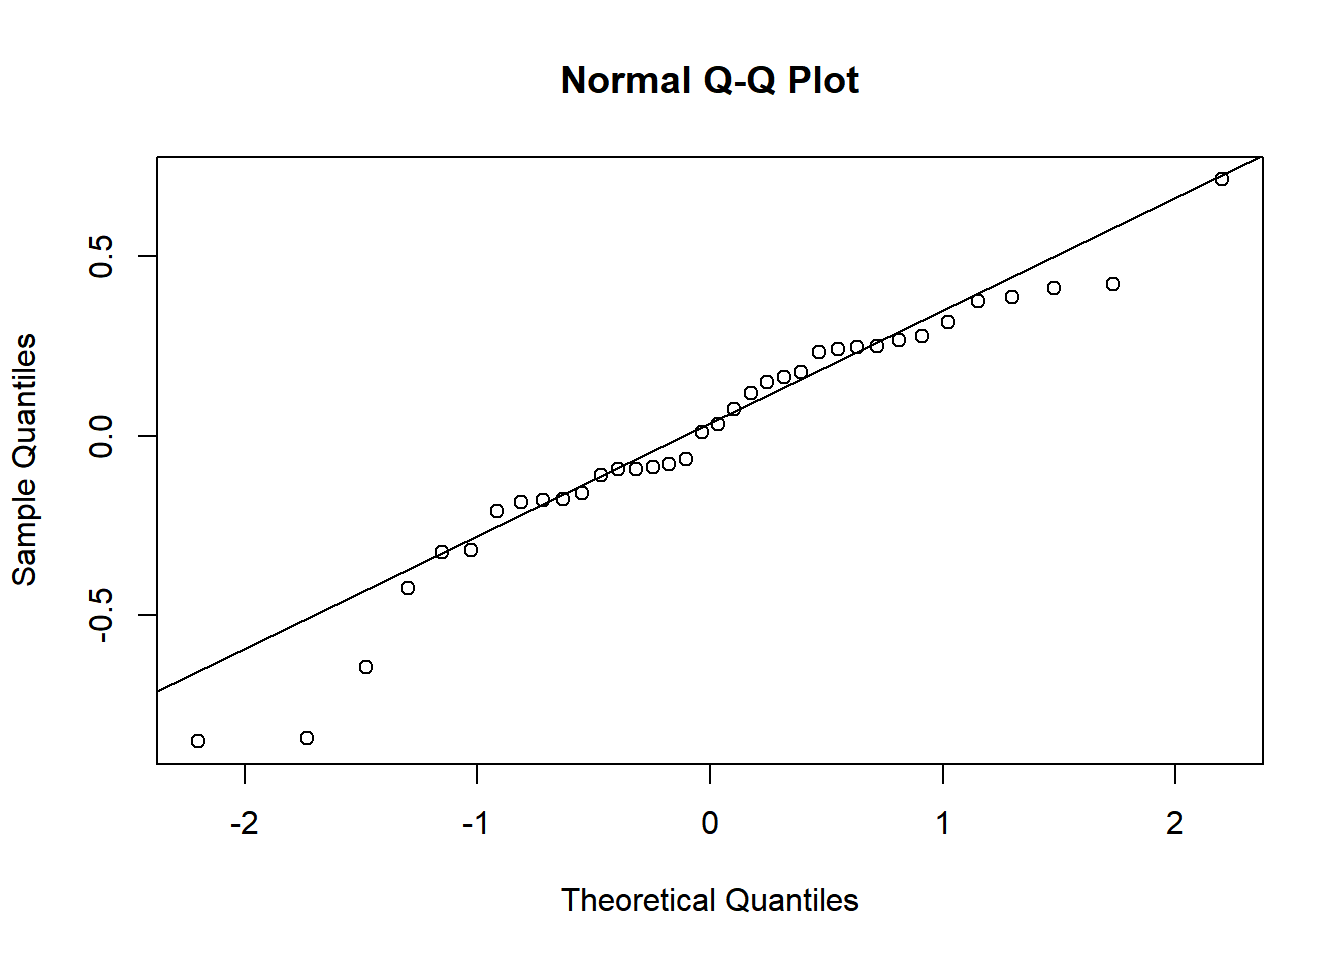
\includegraphics{bookdown-demo_files/figure-latex/unnamed-chunk-92-1.pdf}
In this case the residuals seem to fit the assumption required for
normality.

\subsection{7. Interpret Model}\label{interpret-model-2}

The anova() function only prints the rows of analysis of variance table
for treatment effects when looking at a mixed model fitted using lmer().

\begin{Shaded}
\begin{Highlighting}[]
\KeywordTok{anova}\NormalTok{(rcbdmodel2,}\DataTypeTok{ddf=}\StringTok{"Kenward-Roger"}\NormalTok{)}
\end{Highlighting}
\end{Shaded}

\begin{verbatim}
## Type III Analysis of Variance Table with Kenward-Roger's method
##              Sum Sq Mean Sq NumDF  DenDF F value    Pr(>F)    
## treat        33.253  4.1567     8 23.176 23.6703 2.132e-09 ***
## sqrt(striga)  1.257  1.2568     1 24.977  7.1571   0.01298 *  
## ---
## Signif. codes:  0 '***' 0.001 '**' 0.01 '*' 0.05 '.' 0.1 ' ' 1
\end{verbatim}

ddf=Kenward-Roger tells R which method to use for determining the
calculations of the table; this option matches the defaults found within
SAS or Genstat. The ANOVA table suggests a highly significant effect of
the treatment on the yield.

To obtain the residual variance, and the variance attributed to the
blocks we need an additional command. From these number it is possible
to reconstruct a more classic ANOVA table, if so desired.

\begin{Shaded}
\begin{Highlighting}[]
\KeywordTok{print}\NormalTok{(}\KeywordTok{VarCorr}\NormalTok{(rcbdmodel2), }\DataTypeTok{comp=}\NormalTok{(}\StringTok{"Variance"}\NormalTok{))}
\end{Highlighting}
\end{Shaded}

\begin{verbatim}
##  Groups   Name        Variance
##  rep      (Intercept) 0.054136
##  Residual             0.175600
\end{verbatim}

\subsection{8. Present the results from the
model}\label{present-the-results-from-the-model-2}

To help understand what the significant result from the ANOVA table
means we can produce several plots and tables to help us. First we can
use the function emmip() to produce plots of the modelled results,
including 95\% confidence intervals.

\begin{Shaded}
\begin{Highlighting}[]
\KeywordTok{emmip}\NormalTok{(rcbdmodel2,striga}\OperatorTok{~}\NormalTok{treat,}\DataTypeTok{var=}\StringTok{"striga"}\NormalTok{,}\DataTypeTok{CIs =} \OtherTok{TRUE}\NormalTok{, }\DataTypeTok{at =} \KeywordTok{list}\NormalTok{(}\DataTypeTok{striga =} \KeywordTok{c}\NormalTok{(}\DecValTok{0}\NormalTok{, }\DecValTok{10}\NormalTok{,}\DecValTok{100}\NormalTok{,}\DecValTok{1000}\NormalTok{)))}
\end{Highlighting}
\end{Shaded}

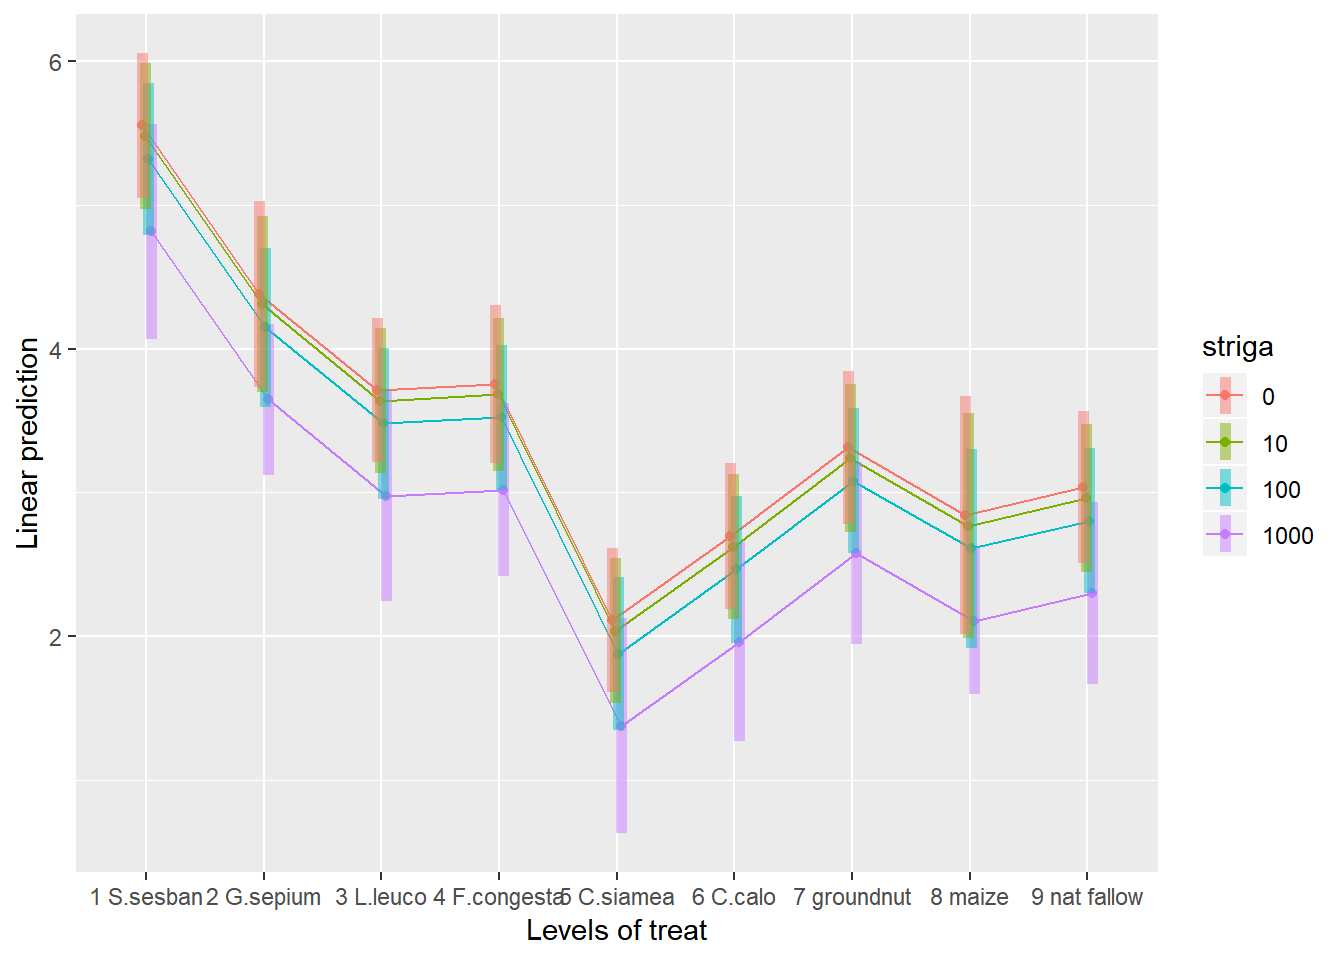
\includegraphics{bookdown-demo_files/figure-latex/unnamed-chunk-95-1.pdf}

Or alternatively

\begin{Shaded}
\begin{Highlighting}[]
\KeywordTok{emmip}\NormalTok{(rcbdmodel2,treat}\OperatorTok{~}\NormalTok{striga,}\DataTypeTok{var=}\StringTok{"striga"}\NormalTok{,}\DataTypeTok{at =} \KeywordTok{list}\NormalTok{(}\DataTypeTok{striga =} \KeywordTok{seq}\NormalTok{(}\DecValTok{0}\NormalTok{,}\DecValTok{1000}\NormalTok{,}\DataTypeTok{by=}\DecValTok{100}\NormalTok{)))}
\end{Highlighting}
\end{Shaded}

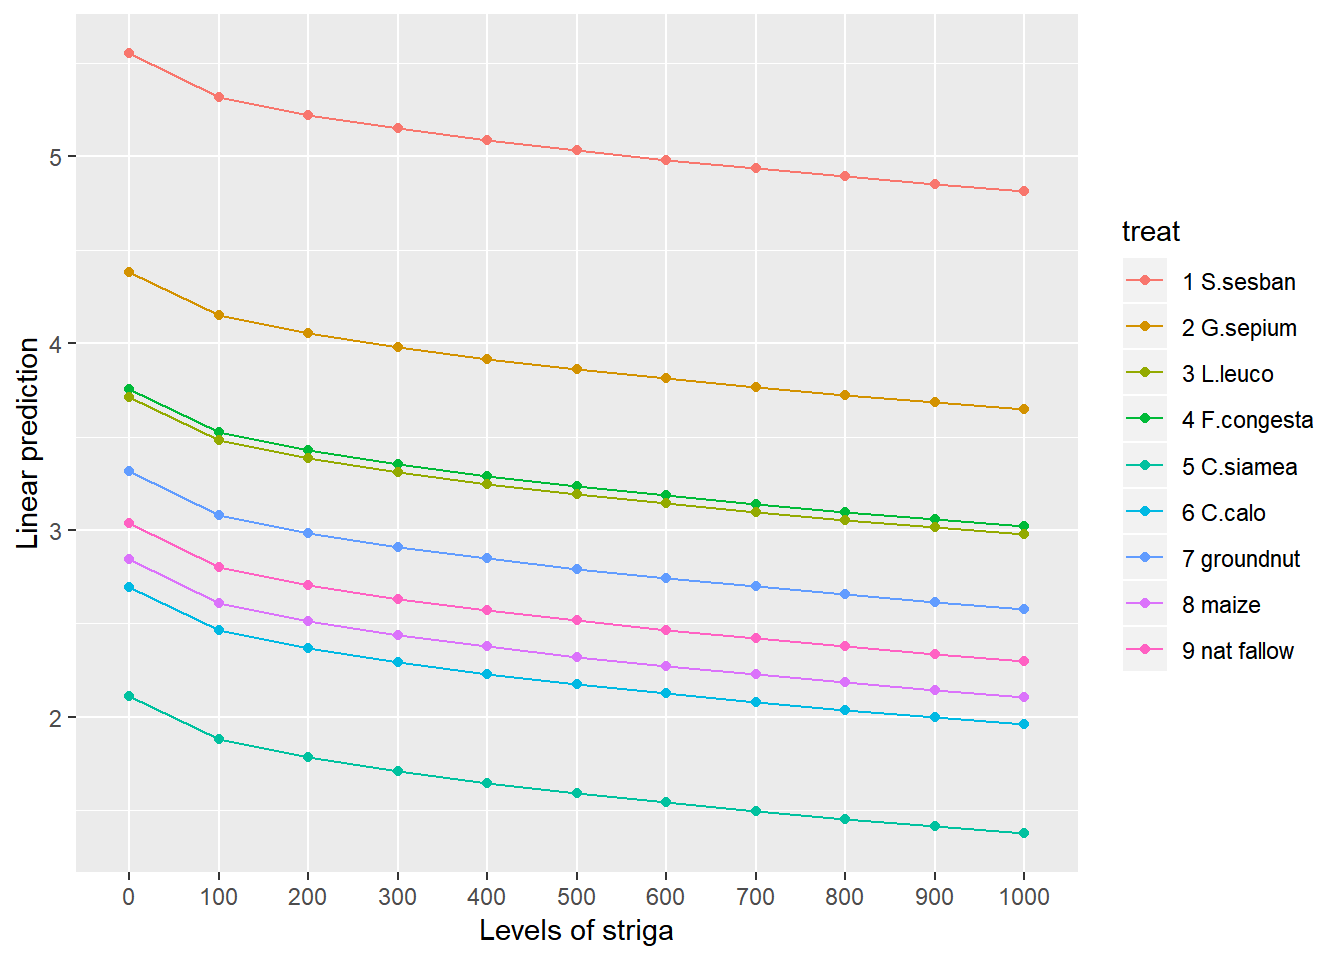
\includegraphics{bookdown-demo_files/figure-latex/unnamed-chunk-96-1.pdf}

To obtain the numbers used in creating this graph we can use the
function emmeans.

\begin{Shaded}
\begin{Highlighting}[]
\KeywordTok{emmeans}\NormalTok{(rcbdmodel2,}\OperatorTok{~}\NormalTok{treat}\OperatorTok{*}\NormalTok{striga,}\DataTypeTok{var=}\StringTok{"striga"}\NormalTok{,}\DataTypeTok{at =} \KeywordTok{list}\NormalTok{(}\DataTypeTok{striga =} \KeywordTok{c}\NormalTok{(}\DecValTok{0}\NormalTok{, }\DecValTok{10}\NormalTok{,}\DecValTok{100}\NormalTok{,}\DecValTok{1000}\NormalTok{)))}
\end{Highlighting}
\end{Shaded}

\begin{verbatim}
##  treat        striga   emmean        SE    df  lower.CL upper.CL
##  1 S.sesban        0 5.553321 0.2396638 18.13 5.0500620 6.056579
##  2 G.sepium        0 4.382568 0.3127465 23.61 3.7365259 5.028609
##  3 L.leuco         0 3.712270 0.2400585 18.17 3.2082694 4.216271
##  4 F.congesta      0 3.755253 0.2638447 20.52 3.2057709 4.304734
##  5 C.siamea        0 2.110821 0.2396638 18.13 1.6075620 2.614079
##  6 C.calo          0 2.696189 0.2430732 18.50 2.1865045 3.205873
##  7 groundnut       0 3.313834 0.2547769 19.69 2.7818499 3.845819
##  8 maize           0 2.842226 0.4031321 25.65 2.0130321 3.671421
##  9 nat fallow      0 3.035732 0.2540738 19.63 2.5050969 3.566367
##  1 S.sesban       10 5.479695 0.2409904 18.28 4.9739401 5.985450
##  2 G.sepium       10 4.308942 0.2958172 22.77 3.6966556 4.921228
##  3 L.leuco        10 3.638644 0.2400389 18.17 3.1346806 4.142608
##  4 F.congesta     10 3.681627 0.2535683 19.58 3.1519610 4.211293
##  5 C.siamea       10 2.037195 0.2409904 18.28 1.5314401 2.542950
##  6 C.calo         10 2.622563 0.2400121 18.17 2.1186500 3.126477
##  7 groundnut      10 3.240209 0.2467978 18.90 2.7234660 3.756951
##  8 maize          10 2.768601 0.3813535 25.41 1.9838290 3.553372
##  9 nat fallow     10 2.962106 0.2463060 18.85 2.4462979 3.477915
##  1 S.sesban      100 5.320496 0.2542321 19.64 4.7895569 5.851435
##  2 G.sepium      100 4.149743 0.2653481 20.65 3.5973441 4.702141
##  3 L.leuco       100 3.479445 0.2505537 19.28 2.9555477 4.003343
##  4 F.congesta    100 3.522428 0.2407873 18.25 3.0170555 4.027800
##  5 C.siamea      100 1.877996 0.2542321 19.64 1.3470569 2.408935
##  6 C.calo        100 2.463364 0.2441046 18.61 1.9517290 2.974999
##  7 groundnut     100 3.081010 0.2396546 18.13 2.5777683 3.584251
##  8 maize         100 2.609402 0.3371451 24.49 1.9143072 3.304496
##  9 nat fallow    100 2.802907 0.2396686 18.13 2.2996397 3.306175
##  1 S.sesban     1000 4.817064 0.3632908 25.12 4.0690284 5.565100
##  2 G.sepium     1000 3.646311 0.2508980 19.32 3.1217555 4.170866
##  3 L.leuco      1000 2.976014 0.3545407 24.94 2.2457305 3.706297
##  4 F.congesta   1000 3.018996 0.2908737 22.48 2.4165111 3.621481
##  5 C.siamea     1000 1.374564 0.3632908 25.12 0.6265284 2.122600
##  6 C.calo       1000 1.959932 0.3353532 24.44 1.2684536 2.651411
##  7 groundnut    1000 2.577578 0.3050497 23.25 1.9469164 3.208239
##  8 maize        1000 2.105970 0.2446031 18.67 1.5933909 2.618549
##  9 nat fallow   1000 2.299476 0.3063498 23.32 1.6662200 2.932731
## 
## Degrees-of-freedom method: kenward-roger 
## Confidence level used: 0.95
\end{verbatim}

And one method for conducting mean separation analysis, holding striga
effect constant, we can use the function cld().

\begin{Shaded}
\begin{Highlighting}[]
\KeywordTok{cld}\NormalTok{(}\KeywordTok{emmeans}\NormalTok{(rcbdmodel2, }\OperatorTok{~}\NormalTok{treat))}
\end{Highlighting}
\end{Shaded}

\begin{verbatim}
##  treat          emmean        SE    df lower.CL upper.CL .group
##  5 C.siamea   1.685247 0.2864468 22.21 1.091515 2.278979  1    
##  6 C.calo     2.270615 0.2673279 20.81 1.714369 2.826862  12   
##  8 maize      2.416653 0.2910113 22.49 1.813896 3.019410  123  
##  9 nat fallow 2.610159 0.2510259 19.33 2.085359 3.134958  123  
##  7 groundnut  2.888261 0.2504107 19.27 2.364636 3.411885   234 
##  3 L.leuco    3.286697 0.2801804 21.79 2.705311 3.868082    34 
##  4 F.congesta 3.329679 0.2445546 18.66 2.817192 3.842166    34 
##  2 G.sepium   3.956994 0.2432827 18.53 3.446913 4.467074     45
##  1 S.sesban   5.127747 0.2864468 22.21 4.534015 5.721479      5
## 
## Degrees-of-freedom method: kenward-roger 
## Confidence level used: 0.95 
## P value adjustment: tukey method for comparing a family of 9 estimates 
## significance level used: alpha = 0.05
\end{verbatim}

In the output, groups sharing a letter in the .group are not
statistically different from each other.

\section{Section 3 -- Methodological
Principles}\label{section-3-methodological-principles-2}

When adjusting for covariates it is important to consider if the
covariate being included is something that could be affected by the
treatment variables, or whether it is something which affects the
outcome independent of the treatments. If we were confident that striga
infestation was not impacted by the choice of treatment then in this
analysis

\chapter{Relay Planting Example}\label{relay-planting-example}

\section{Section 1: Steps in analysis using
R}\label{section-1-steps-in-analysis-using-r-3}

\begin{enumerate}
\def\labelenumi{\arabic{enumi}.}
\tightlist
\item
  Install R packages needed
\end{enumerate}

\begin{Shaded}
\begin{Highlighting}[]
\KeywordTok{library}\NormalTok{(ggplot2)}
\KeywordTok{library}\NormalTok{(emmeans)}
\KeywordTok{library}\NormalTok{(doBy)}
\KeywordTok{library}\NormalTok{(lmerTest)}
\KeywordTok{library}\NormalTok{(multcompView)}
\end{Highlighting}
\end{Shaded}

\begin{enumerate}
\def\labelenumi{\arabic{enumi}.}
\setcounter{enumi}{1}
\tightlist
\item
  Import data
\end{enumerate}

\begin{Shaded}
\begin{Highlighting}[]
\NormalTok{relay <-}\StringTok{ }\KeywordTok{read.csv}\NormalTok{(}\StringTok{"C:/Users/Admin/Desktop/RelayP.csv"}\NormalTok{)}
\end{Highlighting}
\end{Shaded}

\begin{enumerate}
\def\labelenumi{\arabic{enumi}.}
\setcounter{enumi}{2}
\tightlist
\item
  Check and update data
\end{enumerate}

\begin{Shaded}
\begin{Highlighting}[]
\KeywordTok{summary}\NormalTok{(relay)}
\KeywordTok{str}\NormalTok{(relay)}
\NormalTok{relay}\OperatorTok{$}\NormalTok{fert<-}\KeywordTok{factor}\NormalTok{(relay}\OperatorTok{$}\NormalTok{fert)}
\end{Highlighting}
\end{Shaded}

\begin{enumerate}
\def\labelenumi{\arabic{enumi}.}
\setcounter{enumi}{3}
\tightlist
\item
  Explore data
\end{enumerate}

\begin{Shaded}
\begin{Highlighting}[]
\KeywordTok{ggplot}\NormalTok{(}\DataTypeTok{data=}\NormalTok{relay,}\KeywordTok{aes}\NormalTok{(}\DataTypeTok{y=}\NormalTok{grain,}\DataTypeTok{x=}\NormalTok{fert))}\OperatorTok{+}\KeywordTok{geom_boxplot}\NormalTok{(}\KeywordTok{aes}\NormalTok{(}\DataTypeTok{colour=}\NormalTok{plantime))}

\KeywordTok{ggplot}\NormalTok{(}\DataTypeTok{data=}\NormalTok{relay,}\KeywordTok{aes}\NormalTok{(}\DataTypeTok{y=}\NormalTok{grain,}\DataTypeTok{x=}\NormalTok{plantime))}\OperatorTok{+}\KeywordTok{geom_boxplot}\NormalTok{(}\KeywordTok{aes}\NormalTok{(}\DataTypeTok{colour=}\NormalTok{fert))}

\KeywordTok{summaryBy}\NormalTok{(grain}\OperatorTok{~}\NormalTok{fert}\OperatorTok{+}\NormalTok{plantime, }\DataTypeTok{data=}\NormalTok{relay, }\DataTypeTok{FUN=}\KeywordTok{c}\NormalTok{(mean,median,sd))}
\end{Highlighting}
\end{Shaded}

\begin{enumerate}
\def\labelenumi{\arabic{enumi}.}
\setcounter{enumi}{4}
\tightlist
\item
  Specify a model for data
\end{enumerate}

\begin{Shaded}
\begin{Highlighting}[]
\NormalTok{relaymodel<-}\KeywordTok{lmer}\NormalTok{(grain}\OperatorTok{~}\NormalTok{plantime}\OperatorTok{*}\NormalTok{fert}\OperatorTok{+}\NormalTok{(}\DecValTok{1}\OperatorTok{|}\NormalTok{rep), }\DataTypeTok{data=}\NormalTok{RelayP)}
\end{Highlighting}
\end{Shaded}

\begin{enumerate}
\def\labelenumi{\arabic{enumi}.}
\setcounter{enumi}{5}
\tightlist
\item
  Check the model
\end{enumerate}

\begin{Shaded}
\begin{Highlighting}[]
\KeywordTok{plot}\NormalTok{(relaymodel)}

\KeywordTok{qqnorm}\NormalTok{(}\KeywordTok{resid}\NormalTok{(relaymodel))}
\KeywordTok{qqline}\NormalTok{(}\KeywordTok{resid}\NormalTok{(relaymodel))}
\end{Highlighting}
\end{Shaded}

\begin{enumerate}
\def\labelenumi{\arabic{enumi}.}
\setcounter{enumi}{6}
\tightlist
\item
  Interpret the model
\end{enumerate}

\begin{Shaded}
\begin{Highlighting}[]
\KeywordTok{anova}\NormalTok{(relaymodel, }\DataTypeTok{ddf=}\StringTok{"Kenward-Roger"}\NormalTok{)}
\KeywordTok{print}\NormalTok{(}\KeywordTok{VarCorr}\NormalTok{(relaymodel), }\DataTypeTok{comp=}\NormalTok{(}\StringTok{"Variance"}\NormalTok{))}
\end{Highlighting}
\end{Shaded}

\begin{enumerate}
\def\labelenumi{\arabic{enumi}.}
\setcounter{enumi}{7}
\tightlist
\item
  Present the results from the model
\end{enumerate}

\begin{Shaded}
\begin{Highlighting}[]
\KeywordTok{emmip}\NormalTok{(relaymodel,fert}\OperatorTok{~}\NormalTok{plantime,}\DataTypeTok{CIs =} \OtherTok{TRUE}\NormalTok{)}
\KeywordTok{emmip}\NormalTok{(relaymodel,}\OperatorTok{~}\NormalTok{fert,}\DataTypeTok{CIs =} \OtherTok{TRUE}\NormalTok{)}
\KeywordTok{emmip}\NormalTok{(relaymodel,}\OperatorTok{~}\NormalTok{plantime,}\DataTypeTok{CIs =} \OtherTok{TRUE}\NormalTok{)}
\KeywordTok{emmeans}\NormalTok{(relaymodel, }\OperatorTok{~}\NormalTok{fert}\OperatorTok{*}\NormalTok{plantime)}
\end{Highlighting}
\end{Shaded}

\section{Section 2: Explanation of
Steps}\label{section-2-explanation-of-steps-3}

\subsection{1. Install R packages
needed}\label{install-r-packages-needed-3}

A number of packages following packages were used during data
exploration and analysis. For a general introduction explaining what R
packages are and how they work, this is a really useful guide
\url{https://www.datacamp.com/community/tutorials/r-packages-guide}. For
each of these packages to be installed, using install.packages(), this
requires a reliable internet connection and a correctly installed
version of R and RStudio. If you are having difficulties installing
these packages please ask for help.

\begin{Shaded}
\begin{Highlighting}[]
\KeywordTok{install.packages}\NormalTok{(}\StringTok{"ggplot2"}\NormalTok{)}
\KeywordTok{library}\NormalTok{(ggplot2)}
\end{Highlighting}
\end{Shaded}

\texttt{ggplot2} This package provides a powerful graphics language for
creating elegant and complex graphs in R.

\begin{Shaded}
\begin{Highlighting}[]
\KeywordTok{install.packages}\NormalTok{(}\StringTok{"emmeans"}\NormalTok{)}
\KeywordTok{library}\NormalTok{(emmeans)}
\end{Highlighting}
\end{Shaded}

\texttt{emmeans} Estimated marginal means (also known as least squares
means) helps provide expected mean values and confidence intervals from
statistical models.

\begin{Shaded}
\begin{Highlighting}[]
\KeywordTok{install.packages}\NormalTok{(}\StringTok{"doBy"}\NormalTok{)}
\KeywordTok{library}\NormalTok{(doBy)}
\end{Highlighting}
\end{Shaded}

\texttt{doBy}Allows easy production of summary statistic tables

\begin{Shaded}
\begin{Highlighting}[]
\KeywordTok{install.packages}\NormalTok{(}\StringTok{"lmerTest"}\NormalTok{)}
\KeywordTok{library}\NormalTok{(lmerTest)}
\end{Highlighting}
\end{Shaded}

\texttt{lmerTest} Allows produce of flexible mixed effects regression
models, similar to REML in Genstat.

\begin{Shaded}
\begin{Highlighting}[]
\KeywordTok{install.packages}\NormalTok{(}\StringTok{"multcompView"}\NormalTok{)}
\KeywordTok{library}\NormalTok{(multcompView)}
\end{Highlighting}
\end{Shaded}

\texttt{multcompView} allows for mean seperation methods on analyses

\subsection{2. Import data}\label{import-data-3}

Our data set saved as a CSV file, so we can use the read.csv commmand to
import the data. We are going to assign the name of the data with R to
be \texttt{fallow2}. Remember in R Studio you could also use the
``Import Dataset'' menu to import a dataset.

\begin{Shaded}
\begin{Highlighting}[]
\NormalTok{relay <-}\StringTok{ }\KeywordTok{read.csv}\NormalTok{(}\StringTok{"C:/Users/Admin/Desktop/RelayP.csv"}\NormalTok{)}
\end{Highlighting}
\end{Shaded}

\subsection{3. Check and update data}\label{check-and-update-data-3}

When reading data into R it is always useful to check that data is in
the format expected. How many variables are there? How many rows? How
have the columns been read in? The summary command can help to show if
the data is being treated correctly.

\begin{Shaded}
\begin{Highlighting}[]
\KeywordTok{summary}\NormalTok{(relay)}
\end{Highlighting}
\end{Shaded}

\begin{verbatim}
##      rep          plot       plantime       fert        distance    
##  repl 1:27   plot 1 : 3   control: 9   Min.   :  0   Min.   : 0.00  
##  repl 2:27   plot 10: 3   p1     :18   1st Qu.:  0   1st Qu.: 8.00  
##  repl 3:27   plot 11: 3   p2     :18   Median : 50   Median :16.00  
##              plot 12: 3   p3     :18   Mean   : 50   Mean   :15.78  
##              plot 13: 3   p4     :18   3rd Qu.:100   3rd Qu.:23.00  
##              plot 14: 3                Max.   :100   Max.   :31.00  
##              (Other):63                                             
##      grain      
##  Min.   :0.642  
##  1st Qu.:1.905  
##  Median :5.104  
##  Mean   :4.399  
##  3rd Qu.:6.085  
##  Max.   :8.614  
## 
\end{verbatim}

Where data is being treated as a numeric variable (i.e.~a number)
\texttt{summary} provides statistics like the mean, min and max. Where
data is being treated like a categorical variable (i.e.~a group) then
summary provides frequency tables.

From the results we can see that the variables rep and plot are being
considered as numeric variables. However these are grouping variables,
not number variables, the numbers used are simply codes. If we do not
rectify this then our analysis later will be incorrect and
meaningless.\\
This can also be seen more explicitly using the str() function.

\begin{Shaded}
\begin{Highlighting}[]
\KeywordTok{str}\NormalTok{(relay)}
\end{Highlighting}
\end{Shaded}

\begin{verbatim}
## 'data.frame':    81 obs. of  6 variables:
##  $ rep     : Factor w/ 3 levels "repl 1","repl 2",..: 1 1 1 1 1 1 1 1 1 1 ...
##  $ plot    : Factor w/ 27 levels "plot 1","plot 10",..: 1 12 21 22 23 24 25 26 27 2 ...
##  $ plantime: Factor w/ 5 levels "control","p1",..: 5 5 4 1 5 4 3 5 5 1 ...
##  $ fert    : int  50 0 50 100 100 0 0 50 0 0 ...
##  $ distance: int  1 2 3 4 5 6 7 8 9 10 ...
##  $ grain   : num  6.84 2.44 5.2 6.49 6.08 ...
\end{verbatim}

So we need to convert these variables into factors.

\begin{Shaded}
\begin{Highlighting}[]
\NormalTok{relay}\OperatorTok{$}\NormalTok{fert<-}\KeywordTok{factor}\NormalTok{(relay}\OperatorTok{$}\NormalTok{fert)}
\end{Highlighting}
\end{Shaded}

These commands take the column rep within the data frame fallow,
converts into a factor and saves the result in a column called rep
within fallow.

\subsection{4. Explore data}\label{explore-data-3}

\subsubsection{Plots}\label{plots-3}

We are now interesting in assessing the relationship between yield and
striga - so we want to produce a plot of striga against yield, with
different coloured points denoting each treatment.

\begin{Shaded}
\begin{Highlighting}[]
\KeywordTok{ggplot}\NormalTok{(}\DataTypeTok{data=}\NormalTok{relay,}\KeywordTok{aes}\NormalTok{(}\DataTypeTok{y=}\NormalTok{grain,}\DataTypeTok{x=}\NormalTok{fert))}\OperatorTok{+}\KeywordTok{geom_boxplot}\NormalTok{(}\KeywordTok{aes}\NormalTok{(}\DataTypeTok{colour=}\NormalTok{plantime))}
\end{Highlighting}
\end{Shaded}

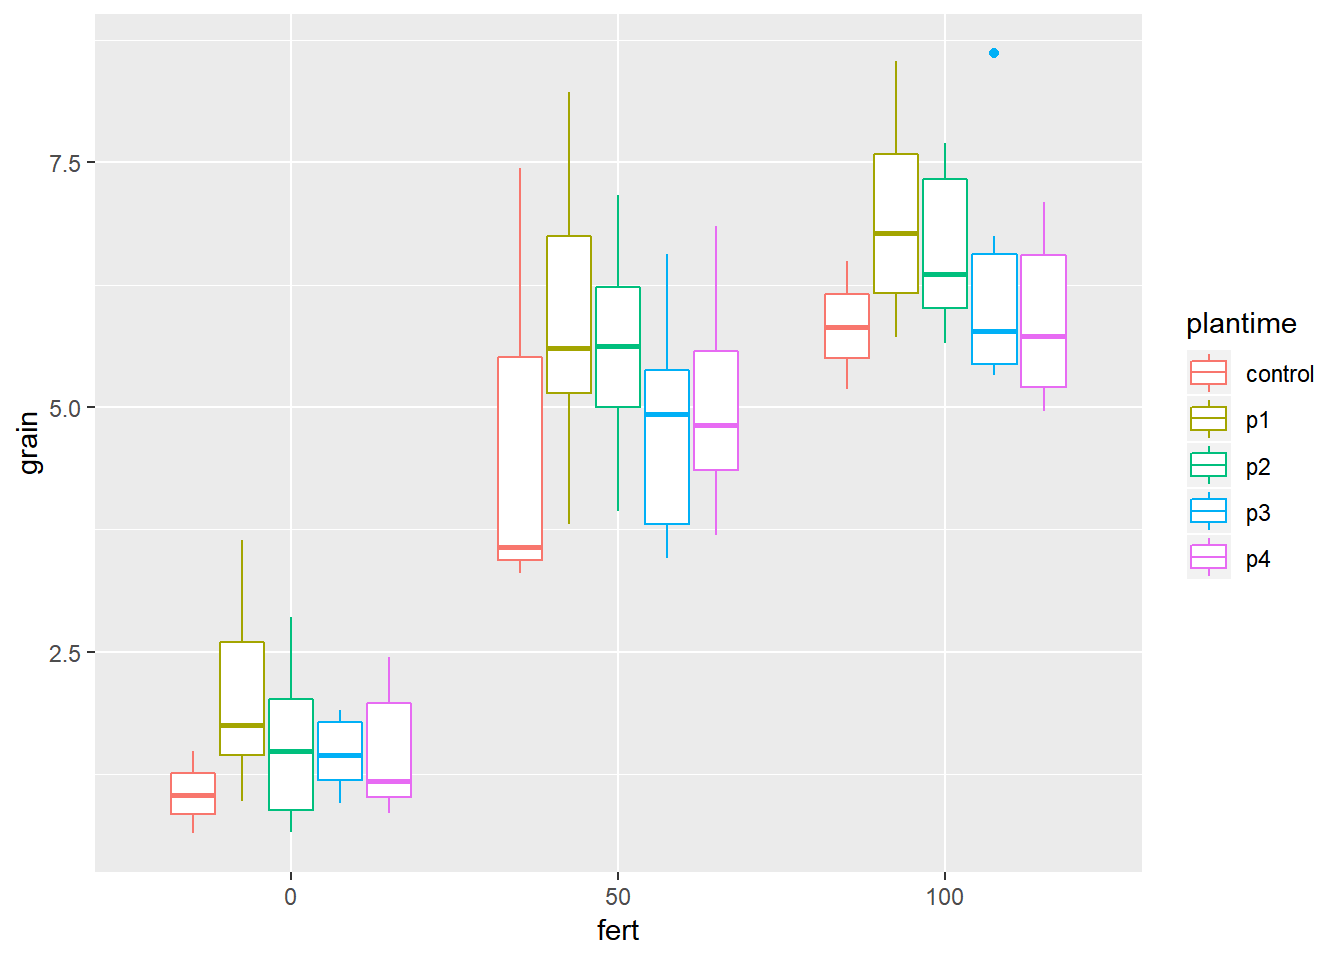
\includegraphics{bookdown-demo_files/figure-latex/unnamed-chunk-118-1.pdf}
We can see from the distribution of striga that there are some farms
with very high levels of striga, and some farms with no striga. The big
range of values makes it hard to make interpretations from this plot, so
taking a square root transformation may help to visualise the
relationship. A log transformation will not help here because of the
large number of 0 values of striga.

\begin{Shaded}
\begin{Highlighting}[]
\KeywordTok{ggplot}\NormalTok{(}\DataTypeTok{data=}\NormalTok{relay,}\KeywordTok{aes}\NormalTok{(}\DataTypeTok{y=}\NormalTok{grain,}\DataTypeTok{x=}\NormalTok{plantime))}\OperatorTok{+}\KeywordTok{geom_boxplot}\NormalTok{(}\KeywordTok{aes}\NormalTok{(}\DataTypeTok{colour=}\NormalTok{fert))}
\end{Highlighting}
\end{Shaded}

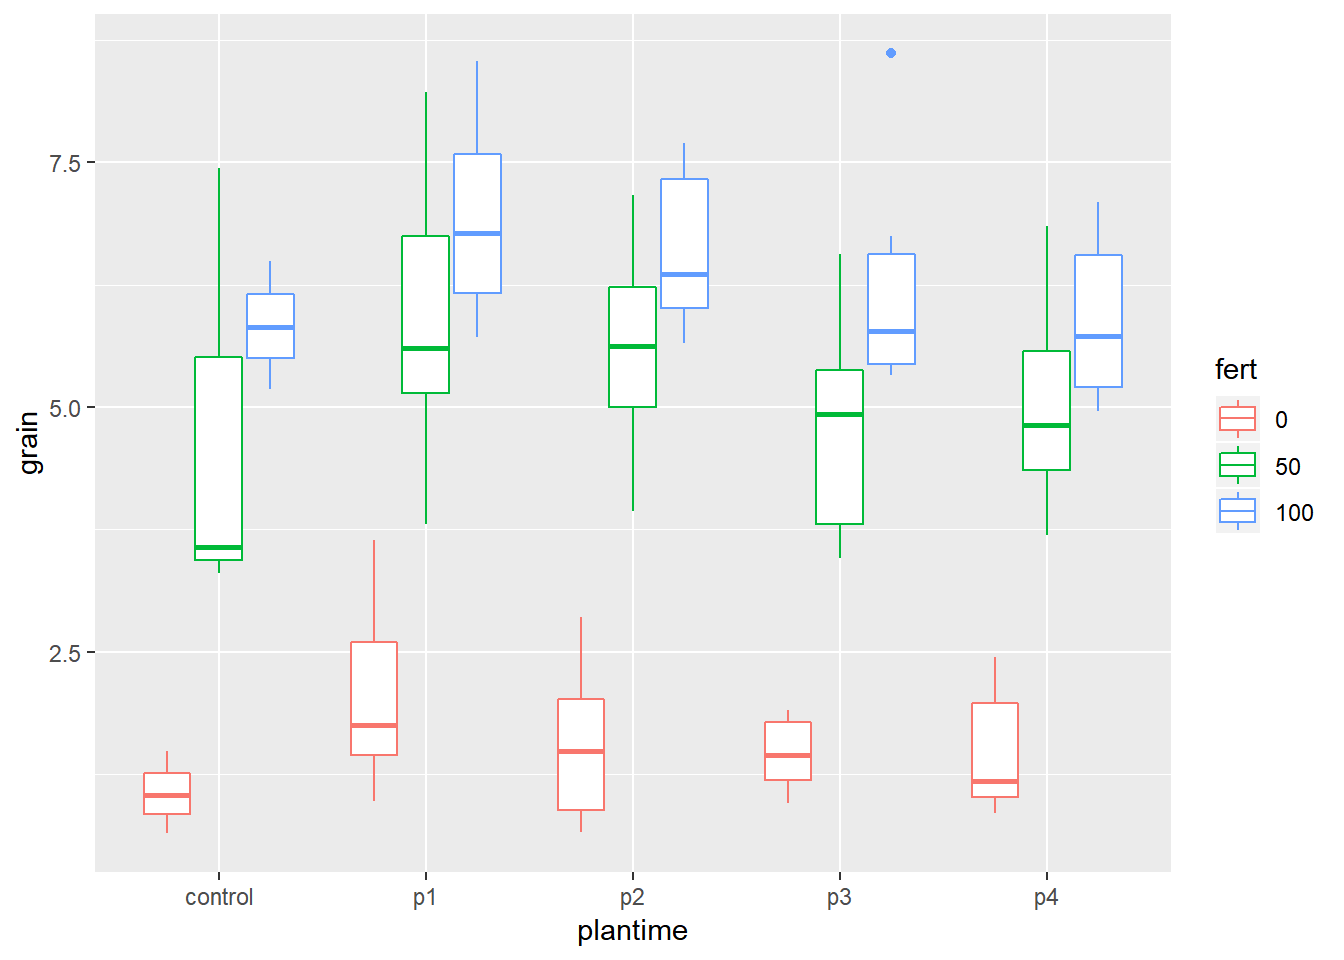
\includegraphics{bookdown-demo_files/figure-latex/unnamed-chunk-119-1.pdf}

\subsubsection{Summary Statistics}\label{summary-statistics-2}

To produce summary statistics, by group, there are many options within
R. One option is to use the summaryBy function, from the doBy library.
The code used for this is quite similar to the code we will use to
produce models in a later step.

\begin{Shaded}
\begin{Highlighting}[]
\KeywordTok{summaryBy}\NormalTok{(grain}\OperatorTok{~}\NormalTok{fert}\OperatorTok{+}\NormalTok{plantime, }\DataTypeTok{data=}\NormalTok{relay, }\DataTypeTok{FUN=}\KeywordTok{c}\NormalTok{(mean,median,sd))}
\end{Highlighting}
\end{Shaded}

\begin{verbatim}
##    fert plantime grain.mean grain.median  grain.sd
## 1     0  control   1.052333       1.0340 0.4198003
## 2     0       p1   2.055333       1.7495 0.9954934
## 3     0       p2   1.559667       1.4835 0.8458025
## 4     0       p3   1.457000       1.4465 0.3850964
## 5     0       p4   1.474500       1.1820 0.6817175
## 6    50  control   4.769000       3.5660 2.3196256
## 7    50       p1   5.890000       5.5995 1.5543606
## 8    50       p2   5.592000       5.6170 1.1410732
## 9    50       p3   4.804333       4.9295 1.1960488
## 10   50       p4   5.030500       4.8130 1.1319579
## 11  100  control   5.831667       5.8200 0.6525782
## 12  100       p1   6.934000       6.7720 1.0728338
## 13  100       p2   6.603667       6.3615 0.8626484
## 14  100       p3   6.272167       5.7760 1.2615166
## 15  100       p4   5.890833       5.7235 0.8759115
\end{verbatim}

\subsection{5. Specify a model for
data}\label{specify-a-model-for-data-3}

In this design, an RCBD, we have one treatment factor, ``treat'', and
one layout factor ``rep''. More information about model fitting can be
found in section 2.

\begin{Shaded}
\begin{Highlighting}[]
\NormalTok{relaymodel<-}\KeywordTok{lmer}\NormalTok{(grain}\OperatorTok{~}\NormalTok{plantime}\OperatorTok{*}\NormalTok{fert}\OperatorTok{+}\NormalTok{(}\DecValTok{1}\OperatorTok{|}\NormalTok{rep), }\DataTypeTok{data=}\NormalTok{relay)}
\end{Highlighting}
\end{Shaded}

R is unlike many other software packages in how it fits models. The best
way of handling models in R is to assign the model to a name (in this
case rcbdmodel1) and then ask R to provide different sorts of output for
this model. When you run the above line you will get now output from the
data - this is what we expected to see!

\subsection{6. Check the model}\label{check-the-model-3}

Before interpretting the model any further we should investigate the
model validity, to ensure any conclusions we draw are valid. There are 3
assumptions that we can check for using standard model checking plots.
1. Homogeneity (equal variance) 2. Values with high leverage 3.
Normality of residuals

The function plot() when used with a model will plot the fitted values
from the model against the expected values.

\begin{Shaded}
\begin{Highlighting}[]
\KeywordTok{plot}\NormalTok{(relaymodel)}
\end{Highlighting}
\end{Shaded}

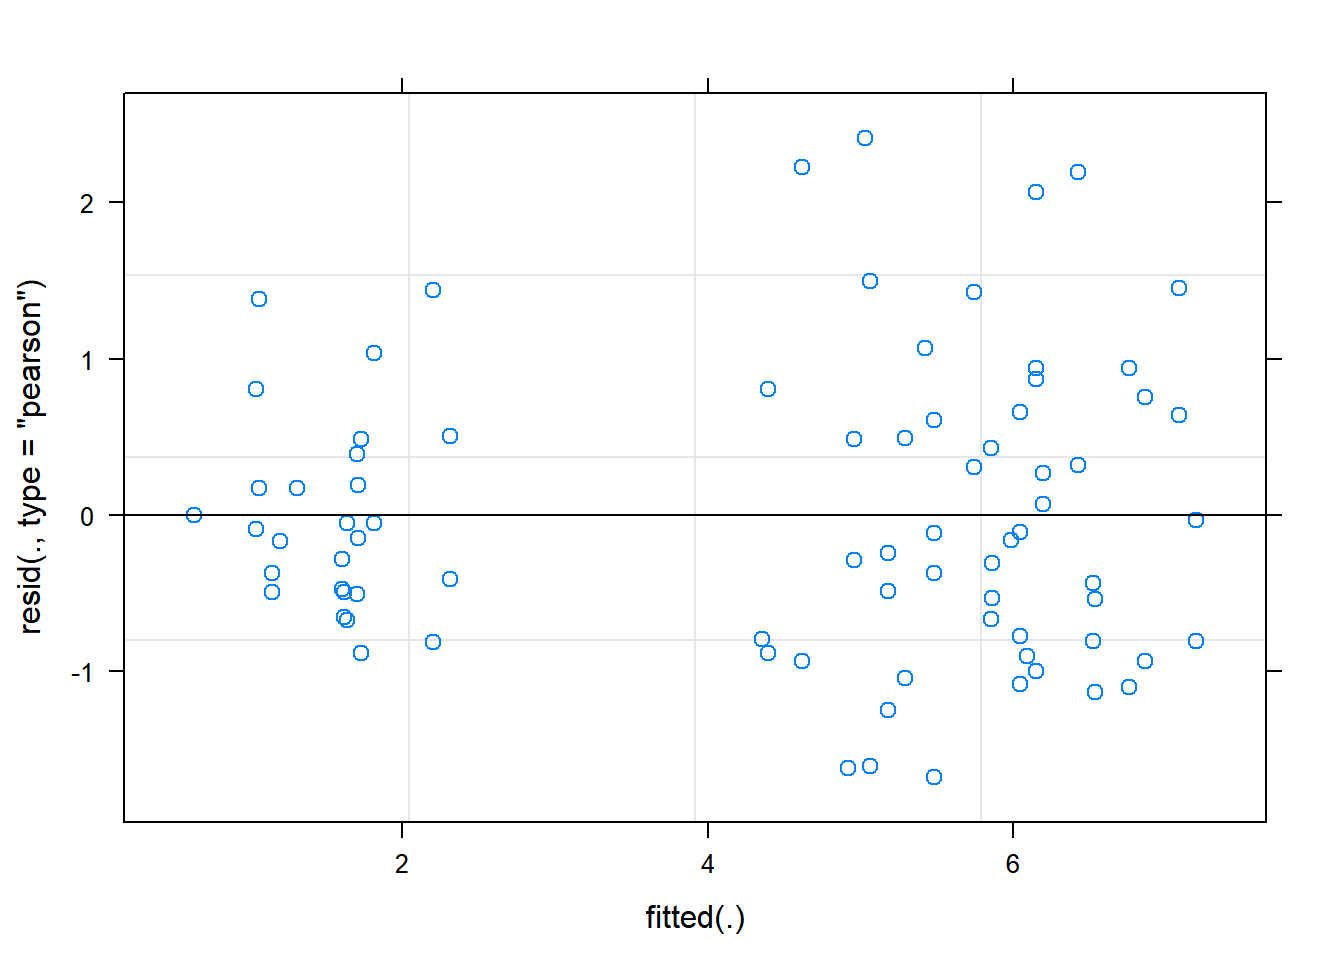
\includegraphics{bookdown-demo_files/figure-latex/unnamed-chunk-122-1.pdf}
The residual Vs fitted plot is a scatter plot of the Residuals on the
y-axis and the fitted on the x-axis and the aim for this plot is to test
the assumption of equal variance of the residuals across the range of
fitted values. Since the residuals do not funnel out (to form
triangular/diamond shape) the assumption of equal variance is met.

We can also see that there are no extreme values in the residuals which
might be potentially causing problems with the validity of our
conclusions (leverage)

To assess the assumption of normality we can produce a qqplot. This
shows us how closely the residuals follow a normal distribution - if
there are severe and syste,matic deviations from the line then we may
want to consider an alternative distribution.

\begin{Shaded}
\begin{Highlighting}[]
\KeywordTok{qqnorm}\NormalTok{(}\KeywordTok{resid}\NormalTok{(relaymodel))}
\KeywordTok{qqline}\NormalTok{(}\KeywordTok{resid}\NormalTok{(relaymodel))}
\end{Highlighting}
\end{Shaded}

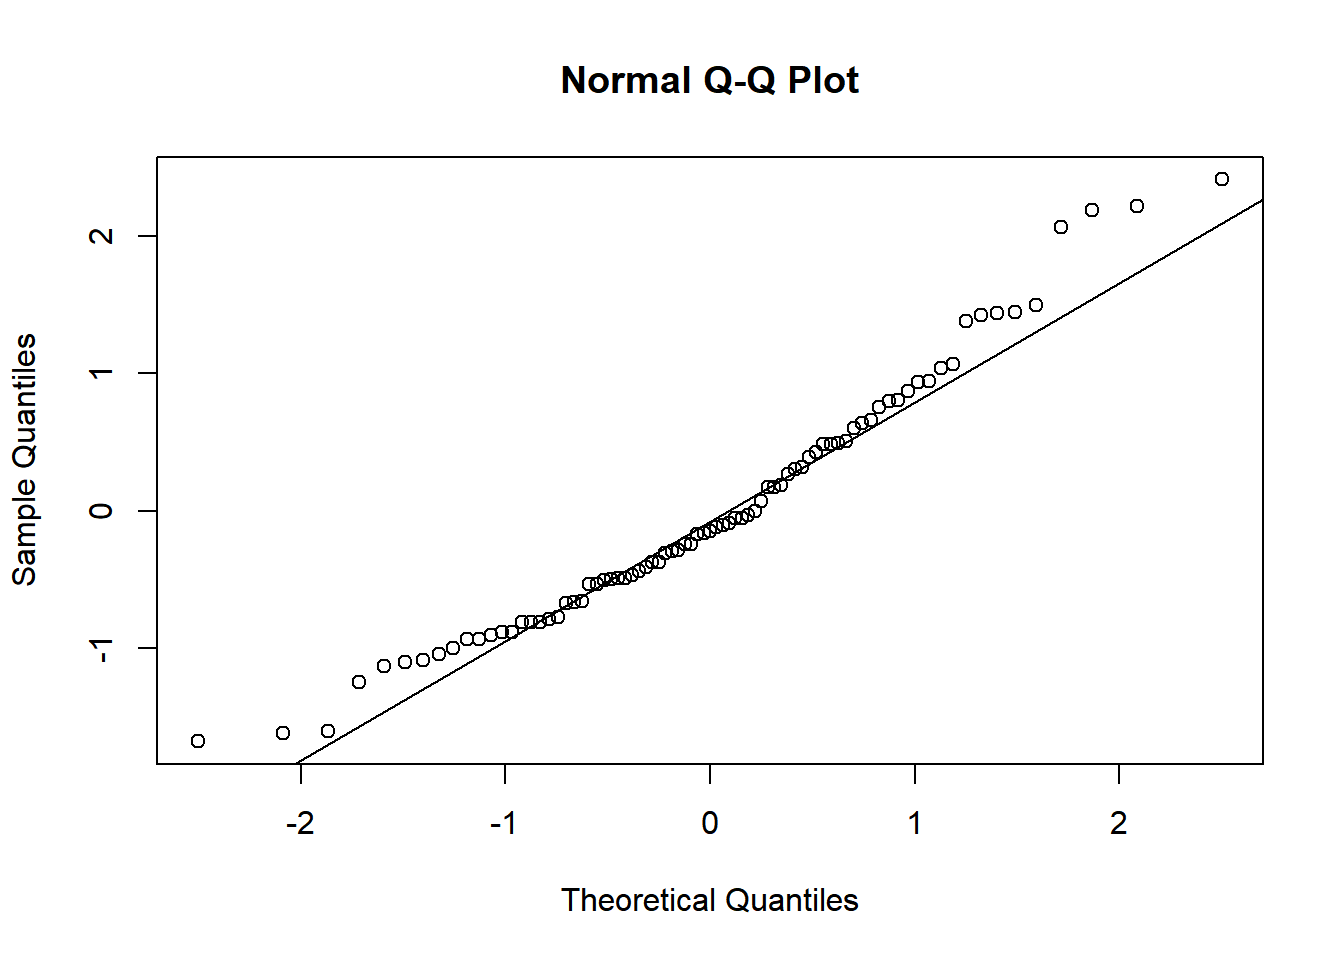
\includegraphics{bookdown-demo_files/figure-latex/unnamed-chunk-123-1.pdf}
In this case the residuals seem to fit the assumption required for
normality.

\subsection{7. Interpret Model}\label{interpret-model-3}

The anova() function only prints the rows of analysis of variance table
for treatment effects when looking at a mixed model fitted using lmer().

\begin{Shaded}
\begin{Highlighting}[]
\KeywordTok{anova}\NormalTok{(relaymodel,}\DataTypeTok{ddf=}\StringTok{"Kenward-Roger"}\NormalTok{)}
\end{Highlighting}
\end{Shaded}

\begin{verbatim}
## Type III Analysis of Variance Table with Kenward-Roger's method
##                Sum Sq Mean Sq NumDF DenDF  F value  Pr(>F)    
## plantime       10.832   2.708     4    64   2.6160 0.04321 *  
## fert          314.749 157.374     2    64 152.0239 < 2e-16 ***
## plantime:fert   1.381   0.173     8    64   0.1668 0.99451    
## ---
## Signif. codes:  0 '***' 0.001 '**' 0.01 '*' 0.05 '.' 0.1 ' ' 1
\end{verbatim}

ddf=Kenward-Roger tells R which method to use for determining the
calculations of the table; this option matches the defaults found within
SAS or Genstat. The ANOVA table suggests a highly significant effect of
the treatment on the yield.

To obtain the residual variance, and the variance attributed to the
blocks we need an additional command. From these number it is possible
to reconstruct a more classic ANOVA table, if so desired.

\begin{Shaded}
\begin{Highlighting}[]
\KeywordTok{print}\NormalTok{(}\KeywordTok{VarCorr}\NormalTok{(relaymodel), }\DataTypeTok{comp=}\NormalTok{(}\StringTok{"Variance"}\NormalTok{))}
\end{Highlighting}
\end{Shaded}

\begin{verbatim}
##  Groups   Name        Variance
##  rep      (Intercept) 0.16034 
##  Residual             1.03519
\end{verbatim}

\subsection{8. Present the results from the
model}\label{present-the-results-from-the-model-3}

To help understand what the significant result from the ANOVA table
means we can produce several plots and tables to help us. First we can
use the function emmip() to produce plots of the modelled results,
including 95\% confidence intervals.

\begin{Shaded}
\begin{Highlighting}[]
\KeywordTok{emmip}\NormalTok{(relaymodel,fert}\OperatorTok{~}\NormalTok{plantime,}\DataTypeTok{CIs =} \OtherTok{TRUE}\NormalTok{)}
\end{Highlighting}
\end{Shaded}

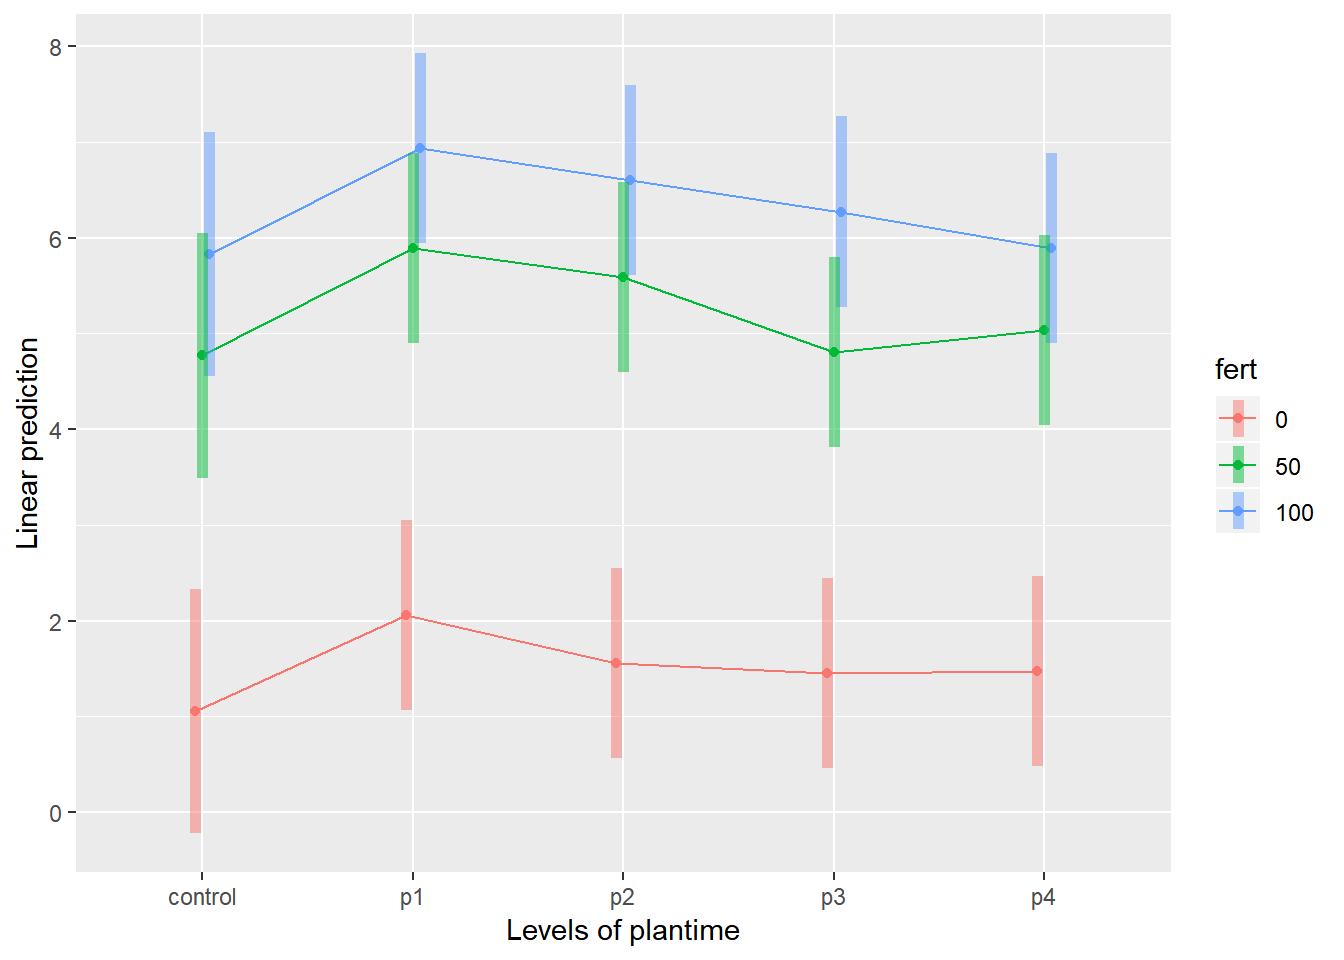
\includegraphics{bookdown-demo_files/figure-latex/unnamed-chunk-126-1.pdf}

Or alternatively

\begin{Shaded}
\begin{Highlighting}[]
\KeywordTok{emmip}\NormalTok{(relaymodel,}\OperatorTok{~}\NormalTok{fert,}\DataTypeTok{CIs =} \OtherTok{TRUE}\NormalTok{)}
\end{Highlighting}
\end{Shaded}

\begin{verbatim}
## NOTE: Results may be misleading due to involvement in interactions
\end{verbatim}

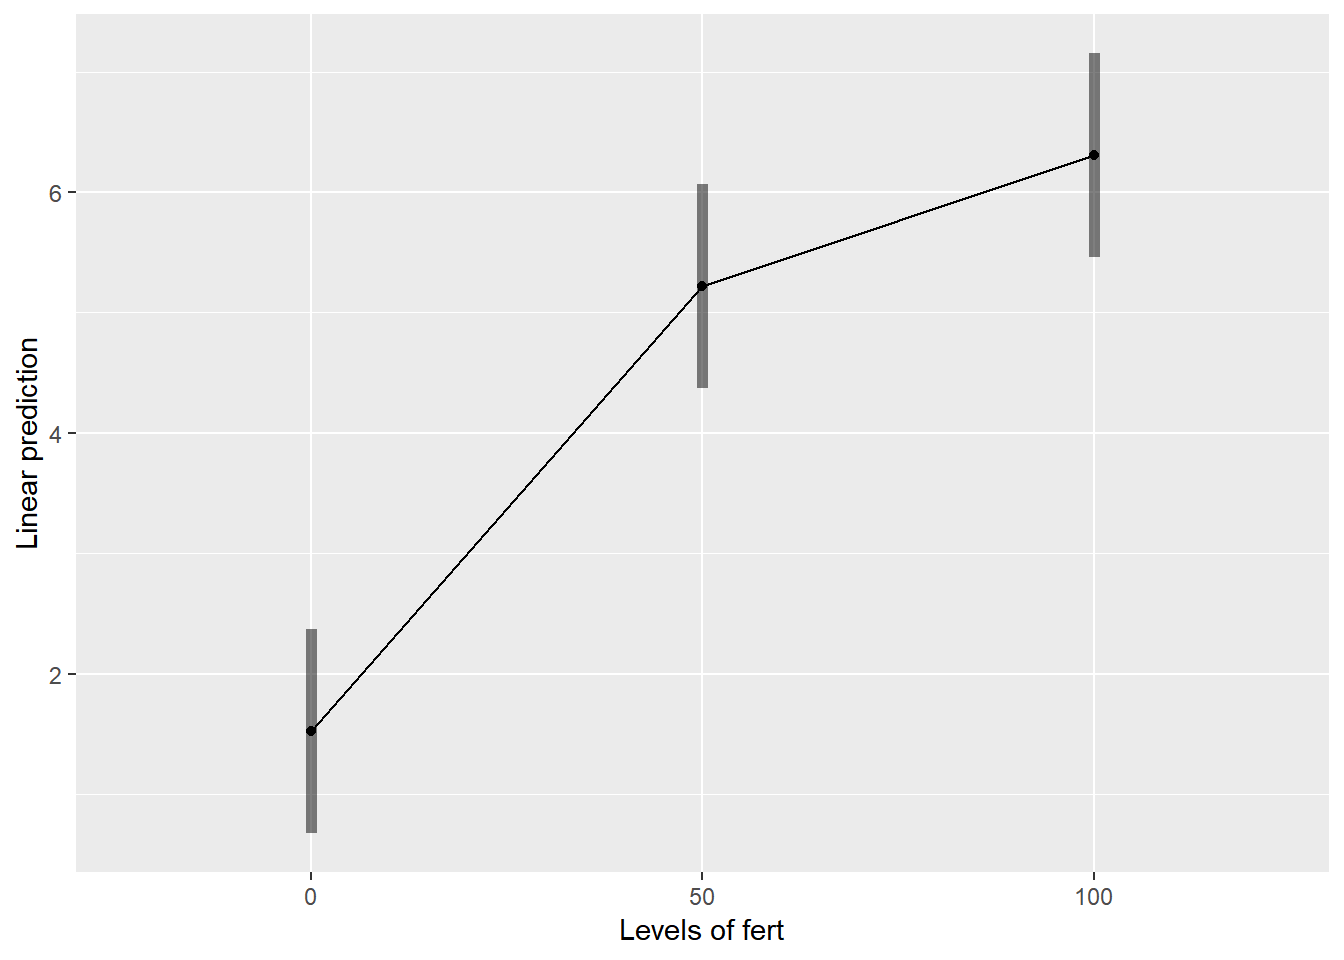
\includegraphics{bookdown-demo_files/figure-latex/unnamed-chunk-127-1.pdf}

\begin{Shaded}
\begin{Highlighting}[]
\KeywordTok{emmip}\NormalTok{(relaymodel,}\OperatorTok{~}\NormalTok{plantime,}\DataTypeTok{CIs =} \OtherTok{TRUE}\NormalTok{)}
\end{Highlighting}
\end{Shaded}

\begin{verbatim}
## NOTE: Results may be misleading due to involvement in interactions
\end{verbatim}

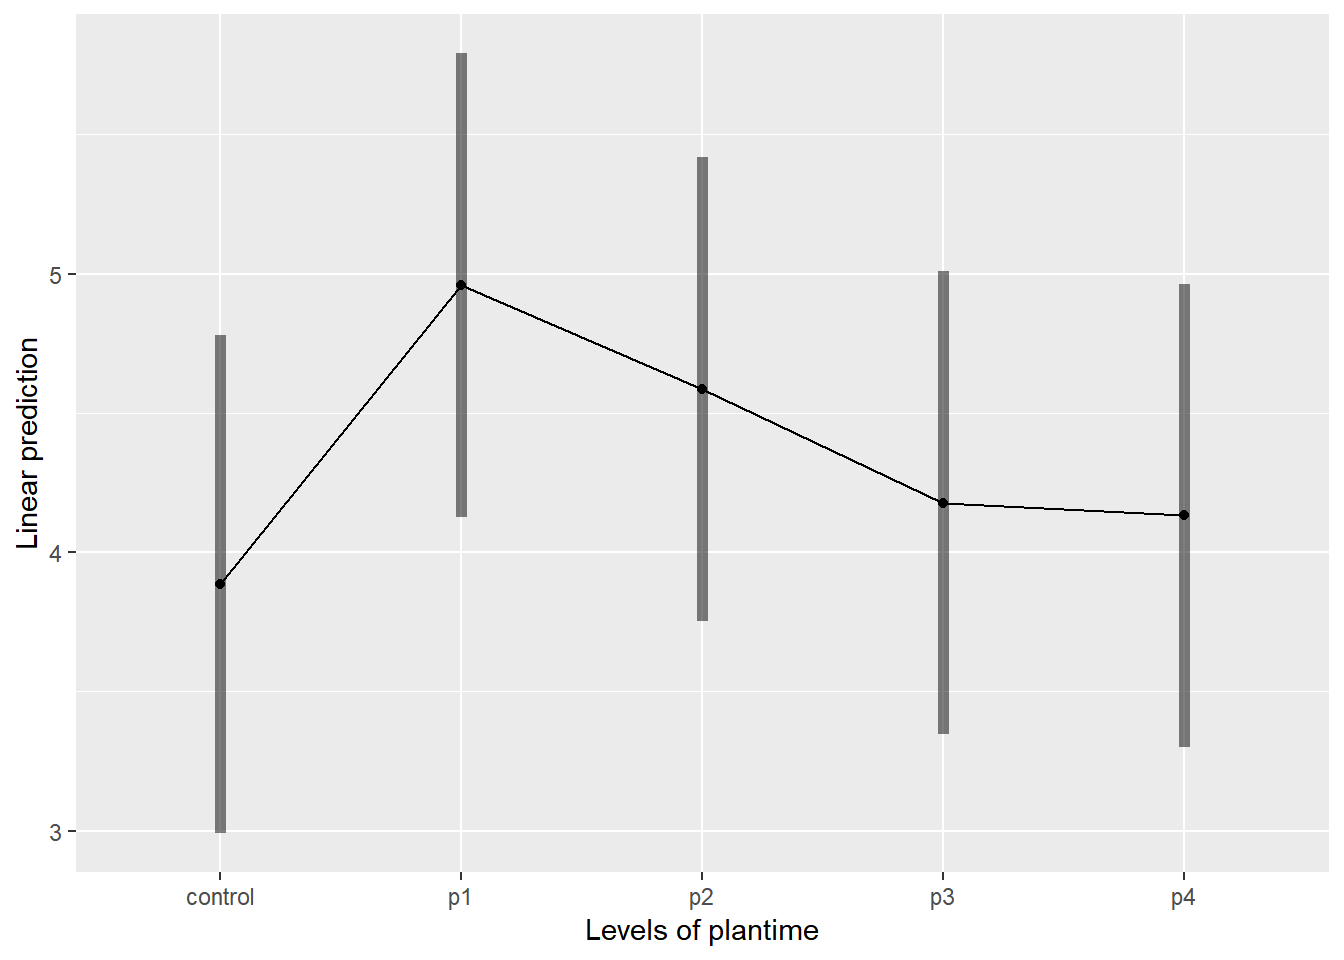
\includegraphics{bookdown-demo_files/figure-latex/unnamed-chunk-127-2.pdf}

To obtain the numbers used in creating this graph we can use the
function emmeans.

\begin{Shaded}
\begin{Highlighting}[]
\KeywordTok{emmeans}\NormalTok{(relaymodel, }\OperatorTok{~}\NormalTok{fert}\OperatorTok{*}\NormalTok{plantime)}
\end{Highlighting}
\end{Shaded}

\begin{verbatim}
##  fert plantime   emmean       SE    df   lower.CL upper.CL
##  0    control  1.052333 0.631278 40.53 -0.2230062 2.327673
##  50   control  4.769000 0.631278 40.53  3.4936605 6.044339
##  100  control  5.831667 0.631278 40.53  4.5563272 7.107006
##  0    p1       2.055333 0.475373 19.70  1.0627645 3.047902
##  50   p1       5.890000 0.475373 19.70  4.8974312 6.882569
##  100  p1       6.934000 0.475373 19.70  5.9414312 7.926569
##  0    p2       1.559667 0.475373 19.70  0.5670979 2.552235
##  50   p2       5.592000 0.475373 19.70  4.5994312 6.584569
##  100  p2       6.603667 0.475373 19.70  5.6110979 7.596235
##  0    p3       1.457000 0.475373 19.70  0.4644312 2.449569
##  50   p3       4.804333 0.475373 19.70  3.8117645 5.796902
##  100  p3       6.272167 0.475373 19.70  5.2795979 7.264735
##  0    p4       1.474500 0.475373 19.70  0.4819312 2.467069
##  50   p4       5.030500 0.475373 19.70  4.0379312 6.023069
##  100  p4       5.890833 0.475373 19.70  4.8982645 6.883402
## 
## Degrees-of-freedom method: kenward-roger 
## Confidence level used: 0.95
\end{verbatim}

And one method for conducting mean separation analysis, holding striga
effect constant, we can use the function cld().

\begin{Shaded}
\begin{Highlighting}[]
\KeywordTok{cld}\NormalTok{(}\KeywordTok{emmeans}\NormalTok{(relaymodel, }\OperatorTok{~}\NormalTok{fert))}
\end{Highlighting}
\end{Shaded}

\begin{verbatim}
## NOTE: Results may be misleading due to involvement in interactions
\end{verbatim}

\begin{verbatim}
##  fert   emmean        SE   df  lower.CL upper.CL .group
##  0    1.519767 0.3079851 4.08 0.6711501 2.368383  1    
##  50   5.217167 0.3079851 4.08 4.3685501 6.065783   2   
##  100  6.306467 0.3079851 4.08 5.4578501 7.155083    3  
## 
## Results are averaged over the levels of: plantime 
## Degrees-of-freedom method: kenward-roger 
## Confidence level used: 0.95 
## P value adjustment: tukey method for comparing a family of 3 estimates 
## significance level used: alpha = 0.05
\end{verbatim}

\begin{Shaded}
\begin{Highlighting}[]
\KeywordTok{cld}\NormalTok{(}\KeywordTok{emmeans}\NormalTok{(relaymodel, }\OperatorTok{~}\NormalTok{plantime))}
\end{Highlighting}
\end{Shaded}

\begin{verbatim}
## NOTE: Results may be misleading due to involvement in interactions
\end{verbatim}

\begin{verbatim}
##  plantime   emmean        SE    df lower.CL upper.CL .group
##  control  3.884333 0.4104494 12.04 2.990409 4.778257  1    
##  p4       4.131944 0.3331034  5.54 3.299984 4.963905  1    
##  p3       4.177833 0.3331034  5.54 3.345873 5.009794  1    
##  p2       4.585111 0.3331034  5.54 3.753151 5.417071  1    
##  p1       4.959778 0.3331034  5.54 4.127817 5.791738  1    
## 
## Results are averaged over the levels of: fert 
## Degrees-of-freedom method: kenward-roger 
## Confidence level used: 0.95 
## P value adjustment: tukey method for comparing a family of 5 estimates 
## significance level used: alpha = 0.05
\end{verbatim}

\begin{Shaded}
\begin{Highlighting}[]
\KeywordTok{cld}\NormalTok{(}\KeywordTok{emmeans}\NormalTok{(relaymodel, }\OperatorTok{~}\NormalTok{fert}\OperatorTok{*}\NormalTok{plantime))}
\end{Highlighting}
\end{Shaded}

\begin{verbatim}
##  fert plantime   emmean       SE    df   lower.CL upper.CL .group
##  0    control  1.052333 0.631278 40.53 -0.2230062 2.327673  1    
##  0    p3       1.457000 0.475373 19.70  0.4644312 2.449569  1    
##  0    p4       1.474500 0.475373 19.70  0.4819312 2.467069  1    
##  0    p2       1.559667 0.475373 19.70  0.5670979 2.552235  1    
##  0    p1       2.055333 0.475373 19.70  1.0627645 3.047902  1    
##  50   control  4.769000 0.631278 40.53  3.4936605 6.044339   23  
##  50   p3       4.804333 0.475373 19.70  3.8117645 5.796902   2   
##  50   p4       5.030500 0.475373 19.70  4.0379312 6.023069   23  
##  50   p2       5.592000 0.475373 19.70  4.5994312 6.584569   23  
##  100  control  5.831667 0.631278 40.53  4.5563272 7.107006   23  
##  50   p1       5.890000 0.475373 19.70  4.8974312 6.882569   23  
##  100  p4       5.890833 0.475373 19.70  4.8982645 6.883402   23  
##  100  p3       6.272167 0.475373 19.70  5.2795979 7.264735   23  
##  100  p2       6.603667 0.475373 19.70  5.6110979 7.596235   23  
##  100  p1       6.934000 0.475373 19.70  5.9414312 7.926569    3  
## 
## Degrees-of-freedom method: kenward-roger 
## Confidence level used: 0.95 
## P value adjustment: tukey method for comparing a family of 15 estimates 
## significance level used: alpha = 0.05
\end{verbatim}

In the output, groups sharing a letter in the .group are not
statistically different from each other.

\section{Section 3 -- Methodological
Principles}\label{section-3-methodological-principles-3}

When adjusting for covariates it is important to consider if the
covariate being included is something that could be affected by the
treatment variables, or whether it is something which affects the
outcome independent of the treatments. If we were confident that striga
infestation was not impacted by the choice of treatment then in this
analysis

\chapter{Multi-Environment Trial
Analysis}\label{multi-environment-trial-analysis}

\section{Section 1: Steps in analysis using
R}\label{section-1-steps-in-analysis-using-r-4}

\begin{enumerate}
\def\labelenumi{\arabic{enumi}.}
\tightlist
\item
  Install R packages needed
\end{enumerate}

\begin{Shaded}
\begin{Highlighting}[]
\KeywordTok{library}\NormalTok{(ggplot2)}
\KeywordTok{library}\NormalTok{(emmeans)}
\KeywordTok{library}\NormalTok{(doBy)}
\KeywordTok{library}\NormalTok{(lmerTest)}
\KeywordTok{library}\NormalTok{(multcompView)}
\end{Highlighting}
\end{Shaded}

\begin{enumerate}
\def\labelenumi{\arabic{enumi}.}
\setcounter{enumi}{1}
\tightlist
\item
  Import data
\end{enumerate}

\begin{Shaded}
\begin{Highlighting}[]
\NormalTok{vartrial <-}\StringTok{ }\KeywordTok{read.csv}\NormalTok{(}\StringTok{"C:/Users/Admin/Desktop/mozvartrial.csv"}\NormalTok{)}
\end{Highlighting}
\end{Shaded}

\begin{enumerate}
\def\labelenumi{\arabic{enumi}.}
\setcounter{enumi}{2}
\tightlist
\item
  Check and update data
\end{enumerate}

\begin{Shaded}
\begin{Highlighting}[]
\KeywordTok{summary}\NormalTok{(vartrial)}
\KeywordTok{str}\NormalTok{(vartrial)}

\NormalTok{vartrial}\OperatorTok{$}\NormalTok{variety<-}\KeywordTok{factor}\NormalTok{(vartrial}\OperatorTok{$}\NormalTok{variety)}
\NormalTok{vartrial}\OperatorTok{$}\NormalTok{trial<-}\KeywordTok{factor}\NormalTok{(vartrial}\OperatorTok{$}\NormalTok{trial)}
\end{Highlighting}
\end{Shaded}

\begin{enumerate}
\def\labelenumi{\arabic{enumi}.}
\setcounter{enumi}{3}
\tightlist
\item
  Explore data
\end{enumerate}

\begin{Shaded}
\begin{Highlighting}[]
\KeywordTok{ggplot}\NormalTok{(}\DataTypeTok{data=}\NormalTok{vartrial,}\KeywordTok{aes}\NormalTok{(}\DataTypeTok{y=}\NormalTok{yield,}\DataTypeTok{x=}\NormalTok{varietyname)) }\OperatorTok{+}
\StringTok{  }\KeywordTok{geom_point}\NormalTok{(}\KeywordTok{aes}\NormalTok{(}\DataTypeTok{colour=}\NormalTok{environment))}

\KeywordTok{ggplot}\NormalTok{(}\DataTypeTok{data=}\NormalTok{vartrial,}\KeywordTok{aes}\NormalTok{(}\DataTypeTok{y=}\NormalTok{yield,}\DataTypeTok{x=}\NormalTok{environment,}\DataTypeTok{colour=}\NormalTok{varietyname,}\DataTypeTok{group=}\NormalTok{varietyname)) }\OperatorTok{+}
\StringTok{  }\KeywordTok{stat_summary}\NormalTok{(}\DataTypeTok{geom=}\StringTok{"line"}\NormalTok{)}

\KeywordTok{ggplot}\NormalTok{(}\DataTypeTok{data=}\NormalTok{vartrial,}\KeywordTok{aes}\NormalTok{(}\DataTypeTok{y=}\NormalTok{yield,}\DataTypeTok{x=}\NormalTok{varietyname))}\OperatorTok{+}
\StringTok{  }\KeywordTok{geom_boxplot}\NormalTok{(}\KeywordTok{aes}\NormalTok{(}\DataTypeTok{colour=}\NormalTok{varietyname))}\OperatorTok{+}\KeywordTok{facet_wrap}\NormalTok{(}\OperatorTok{~}\NormalTok{environment)}


\KeywordTok{summaryBy}\NormalTok{(yield}\OperatorTok{~}\NormalTok{varietyname}\OperatorTok{+}\NormalTok{environment, }\DataTypeTok{data=}\NormalTok{vartrial, }\DataTypeTok{FUN=}\KeywordTok{c}\NormalTok{(mean,median,sd))}
\end{Highlighting}
\end{Shaded}

\begin{enumerate}
\def\labelenumi{\arabic{enumi}.}
\setcounter{enumi}{4}
\tightlist
\item
  Specify a model for data
\end{enumerate}

\begin{Shaded}
\begin{Highlighting}[]
\NormalTok{gxemodel1<-}\KeywordTok{lmer}\NormalTok{(yield}\OperatorTok{~}\NormalTok{varietyname}\OperatorTok{*}\NormalTok{environment}\OperatorTok{+}\NormalTok{(}\DecValTok{1}\OperatorTok{|}\NormalTok{rep}\OperatorTok{:}\NormalTok{environment), }\DataTypeTok{data=}\NormalTok{vartrial)}

\NormalTok{gxemodel2<-}\KeywordTok{lmer}\NormalTok{(yield}\OperatorTok{~}\NormalTok{varietyname}\OperatorTok{*}\NormalTok{environment}\OperatorTok{+}\NormalTok{(}\DecValTok{1}\OperatorTok{|}\NormalTok{rep}\OperatorTok{:}\NormalTok{environment)}\OperatorTok{+}\NormalTok{(}\DecValTok{1}\OperatorTok{|}\NormalTok{rep}\OperatorTok{:}\NormalTok{environment}\OperatorTok{:}\NormalTok{row)}\OperatorTok{+}\NormalTok{(}\DecValTok{1}\OperatorTok{|}\NormalTok{rep}\OperatorTok{:}\NormalTok{environment}\OperatorTok{:}\NormalTok{column), }\DataTypeTok{data=}\NormalTok{vartrial)}

\KeywordTok{anova}\NormalTok{(gxemodel2,gxemodel1)}
\end{Highlighting}
\end{Shaded}

\begin{enumerate}
\def\labelenumi{\arabic{enumi}.}
\setcounter{enumi}{5}
\tightlist
\item
  Check the model
\end{enumerate}

\begin{Shaded}
\begin{Highlighting}[]
\KeywordTok{plot}\NormalTok{(gxemodel2)}

\KeywordTok{qqnorm}\NormalTok{(}\KeywordTok{resid}\NormalTok{(gxemodel2))}
\KeywordTok{qqline}\NormalTok{(}\KeywordTok{resid}\NormalTok{(gxemodel2))}
\end{Highlighting}
\end{Shaded}

\begin{enumerate}
\def\labelenumi{\arabic{enumi}.}
\setcounter{enumi}{6}
\tightlist
\item
  Interpret the model
\end{enumerate}

\begin{Shaded}
\begin{Highlighting}[]
\KeywordTok{anova}\NormalTok{(gxemodel2, }\DataTypeTok{ddf=}\StringTok{"Kenward-Roger"}\NormalTok{)}
\KeywordTok{print}\NormalTok{(}\KeywordTok{VarCorr}\NormalTok{(gxemodel2), }\DataTypeTok{comp=}\NormalTok{(}\StringTok{"Variance"}\NormalTok{))}

\KeywordTok{ranova}\NormalTok{(gxemodel2)}
\end{Highlighting}
\end{Shaded}

\begin{enumerate}
\def\labelenumi{\arabic{enumi}.}
\setcounter{enumi}{7}
\tightlist
\item
  Present the results from the model
\end{enumerate}

\begin{Shaded}
\begin{Highlighting}[]
\KeywordTok{emmip}\NormalTok{(gxemodel2,}\OperatorTok{~}\NormalTok{varietyname}\OperatorTok{|}\NormalTok{environment,}\DataTypeTok{CIs =} \OtherTok{TRUE}\NormalTok{)}

\KeywordTok{emmip}\NormalTok{(gxemodel2,}\OperatorTok{~}\NormalTok{varietyname}\OperatorTok{|}\NormalTok{environment,}\DataTypeTok{CIs =} \OtherTok{TRUE}\NormalTok{)}


\KeywordTok{emmip}\NormalTok{(gxemodel2,varietyname}\OperatorTok{~}\NormalTok{environment)}\OperatorTok{+}\KeywordTok{coord_flip}\NormalTok{()}

\KeywordTok{emmeans}\NormalTok{(gxemodel2, }\OperatorTok{~}\NormalTok{varietyname}\OperatorTok{|}\NormalTok{environment)}

\KeywordTok{cld}\NormalTok{(}\KeywordTok{emmeans}\NormalTok{(gxemodel2, }\OperatorTok{~}\NormalTok{varietyname}\OperatorTok{|}\NormalTok{environment))}

\NormalTok{estimatedmeans<-}\KeywordTok{data.frame}\NormalTok{(}\KeywordTok{cld}\NormalTok{(}\KeywordTok{emmeans}\NormalTok{(gxemodel2, }\OperatorTok{~}\NormalTok{varietyname}\OperatorTok{|}\NormalTok{environment)))}
\NormalTok{estimatedmeans}
\KeywordTok{library}\NormalTok{(reshape2)}
\KeywordTok{dcast}\NormalTok{(varietyname}\OperatorTok{~}\NormalTok{environment,}\DataTypeTok{value.var=}\StringTok{"emmean"}\NormalTok{,}\DataTypeTok{data=}\NormalTok{estimatedmeans)}
\end{Highlighting}
\end{Shaded}

\section{Section 2: Explanation of
Steps}\label{section-2-explanation-of-steps-4}

\subsection{1. Install R packages
needed}\label{install-r-packages-needed-4}

A number of packages following packages were used during data
exploration and analysis. For a general introduction explaining what R
packages are and how they work, this is a really useful guide
\url{https://www.datacamp.com/community/tutorials/r-packages-guide}. For
each of these packages to be installed, using install.packages(), this
requires a reliable internet connection and a correctly installed
version of R and RStudio. If you are having difficulties installing
these packages please ask for help.

\begin{Shaded}
\begin{Highlighting}[]
\KeywordTok{install.packages}\NormalTok{(}\StringTok{"ggplot2"}\NormalTok{)}
\KeywordTok{library}\NormalTok{(ggplot2)}
\end{Highlighting}
\end{Shaded}

\texttt{ggplot2} This package provides a powerful graphics language for
creating elegant and complex graphs in R.

\begin{Shaded}
\begin{Highlighting}[]
\KeywordTok{install.packages}\NormalTok{(}\StringTok{"emmeans"}\NormalTok{)}
\KeywordTok{library}\NormalTok{(emmeans)}
\end{Highlighting}
\end{Shaded}

\texttt{emmeans} Estimated marginal means (also known as least squares
means) helps provide expected mean values and confidence intervals from
statistical models.

\begin{Shaded}
\begin{Highlighting}[]
\KeywordTok{install.packages}\NormalTok{(}\StringTok{"doBy"}\NormalTok{)}
\KeywordTok{library}\NormalTok{(doBy)}
\end{Highlighting}
\end{Shaded}

\texttt{doBy}Allows easy production of summary statistic tables

\begin{Shaded}
\begin{Highlighting}[]
\KeywordTok{install.packages}\NormalTok{(}\StringTok{"lmerTest"}\NormalTok{)}
\KeywordTok{library}\NormalTok{(lmerTest)}
\end{Highlighting}
\end{Shaded}

\texttt{lmerTest} Allows produce of flexible mixed effects regression
models, similar to REML in Genstat.

\begin{Shaded}
\begin{Highlighting}[]
\KeywordTok{install.packages}\NormalTok{(}\StringTok{"multcompView"}\NormalTok{)}
\KeywordTok{library}\NormalTok{(multcompView)}
\end{Highlighting}
\end{Shaded}

\texttt{multcompView} allows for mean seperation methods on analyses

\subsection{2. Import data}\label{import-data-4}

Our data set saved as a CSV file, so we can use the read.csv commmand to
import the data. We are going to assign the name of the data with R to
be \texttt{fallow2}. Remember in R Studio you could also use the
``Import Dataset'' menu to import a dataset.

\begin{Shaded}
\begin{Highlighting}[]
\NormalTok{vartrial <-}\StringTok{ }\KeywordTok{read.csv}\NormalTok{(}\StringTok{"C:/Users/Admin/Desktop/mozvartrial.csv"}\NormalTok{)}
\end{Highlighting}
\end{Shaded}

\subsection{3. Check and update data}\label{check-and-update-data-4}

When reading data into R it is always useful to check that data is in
the format expected. How many variables are there? How many rows? How
have the columns been read in? The summary command can help to show if
the data is being treated correctly.

\begin{Shaded}
\begin{Highlighting}[]
\KeywordTok{summary}\NormalTok{(vartrial)}
\end{Highlighting}
\end{Shaded}

\begin{verbatim}
##      order                   environment     trial        rep      
##  Min.   :  1.00   ChokweIrrigado   :48   Min.   :1   Min.   :1.00  
##  1st Qu.: 84.75   ChokweStressado  :48   1st Qu.:2   1st Qu.:1.75  
##  Median :168.50   Macia_Adelino    :48   Median :4   Median :2.50  
##  Mean   :168.50   Macia_Machava    :48   Mean   :4   Mean   :2.50  
##  3rd Qu.:252.25   Nhacoongo        :48   3rd Qu.:6   3rd Qu.:3.25  
##  Max.   :336.00   UmbeluziIrrigado :48   Max.   :7   Max.   :4.00  
##                   UmbeluziStressado:48                             
##       row            column     variety        varietyname 
##  Min.   :1.000   Min.   :1   Min.   : 1.00   INIA-152: 28  
##  1st Qu.:2.000   1st Qu.:1   1st Qu.: 3.75   INIA-41 : 28  
##  Median :2.500   Median :2   Median : 6.50   INIA-73 : 28  
##  Mean   :2.503   Mean   :2   Mean   : 6.50   IT-16   : 28  
##  3rd Qu.:3.250   3rd Qu.:3   3rd Qu.: 9.25   IT-18   : 28  
##  Max.   :4.000   Max.   :3   Max.   :12.00   IT00K-96: 28  
##                                              (Other) :168  
##     plantnum          yield       
##  Min.   :  4.00   Min.   :  78.2  
##  1st Qu.: 27.00   1st Qu.: 933.3  
##  Median : 44.00   Median :1322.2  
##  Mean   : 50.90   Mean   :1613.9  
##  3rd Qu.: 69.25   3rd Qu.:2253.3  
##  Max.   :141.00   Max.   :4426.7  
## 
\end{verbatim}

Where data is being treated as a numeric variable (i.e.~a number)
\texttt{summary} provides statistics like the mean, min and max. Where
data is being treated like a categorical variable (i.e.~a group) then
summary provides frequency tables.

From the results we can see that the variables rep and plot are being
considered as numeric variables. However these are grouping variables,
not number variables, the numbers used are simply codes. If we do not
rectify this then our analysis later will be incorrect and
meaningless.\\
This can also be seen more explicitly using the str() function.

\begin{Shaded}
\begin{Highlighting}[]
\KeywordTok{str}\NormalTok{(vartrial)}
\end{Highlighting}
\end{Shaded}

\begin{verbatim}
## 'data.frame':    336 obs. of  10 variables:
##  $ order      : int  1 2 3 4 5 6 7 8 9 10 ...
##  $ environment: Factor w/ 7 levels "ChokweIrrigado",..: 1 1 1 1 1 1 1 1 1 1 ...
##  $ trial      : int  1 1 1 1 1 1 1 1 1 1 ...
##  $ rep        : int  1 1 1 1 1 1 1 1 1 1 ...
##  $ row        : int  1 1 1 2 2 2 3 3 3 4 ...
##  $ column     : int  1 2 3 3 2 1 1 2 3 3 ...
##  $ variety    : int  1 2 3 4 5 6 7 8 9 10 ...
##  $ varietyname: Factor w/ 12 levels "INIA-152","INIA-41",..: 12 7 3 11 5 9 6 2 8 4 ...
##  $ plantnum   : int  66 97 77 83 112 106 127 70 128 96 ...
##  $ yield      : num  3404 640 2516 2844 3040 ...
\end{verbatim}

So we need to convert these variables into factors.

\begin{Shaded}
\begin{Highlighting}[]
\NormalTok{vartrial}\OperatorTok{$}\NormalTok{variety<-}\KeywordTok{factor}\NormalTok{(vartrial}\OperatorTok{$}\NormalTok{variety)}
\NormalTok{vartrial}\OperatorTok{$}\NormalTok{trial<-}\KeywordTok{factor}\NormalTok{(vartrial}\OperatorTok{$}\NormalTok{trial)}
\end{Highlighting}
\end{Shaded}

These commands take the column rep within the data frame fallow,
converts into a factor and saves the result in a column called rep
within fallow.

\subsection{4. Explore data}\label{explore-data-4}

\subsubsection{Plots}\label{plots-4}

We are now interesting in assessing the relationship between yield and
striga - so we want to produce a plot of striga against yield, with
different coloured points denoting each treatment.

\begin{Shaded}
\begin{Highlighting}[]
\KeywordTok{ggplot}\NormalTok{(}\DataTypeTok{data=}\NormalTok{vartrial,}\KeywordTok{aes}\NormalTok{(}\DataTypeTok{y=}\NormalTok{yield,}\DataTypeTok{x=}\NormalTok{varietyname)) }\OperatorTok{+}
\StringTok{  }\KeywordTok{geom_point}\NormalTok{(}\KeywordTok{aes}\NormalTok{(}\DataTypeTok{colour=}\NormalTok{environment))}
\end{Highlighting}
\end{Shaded}

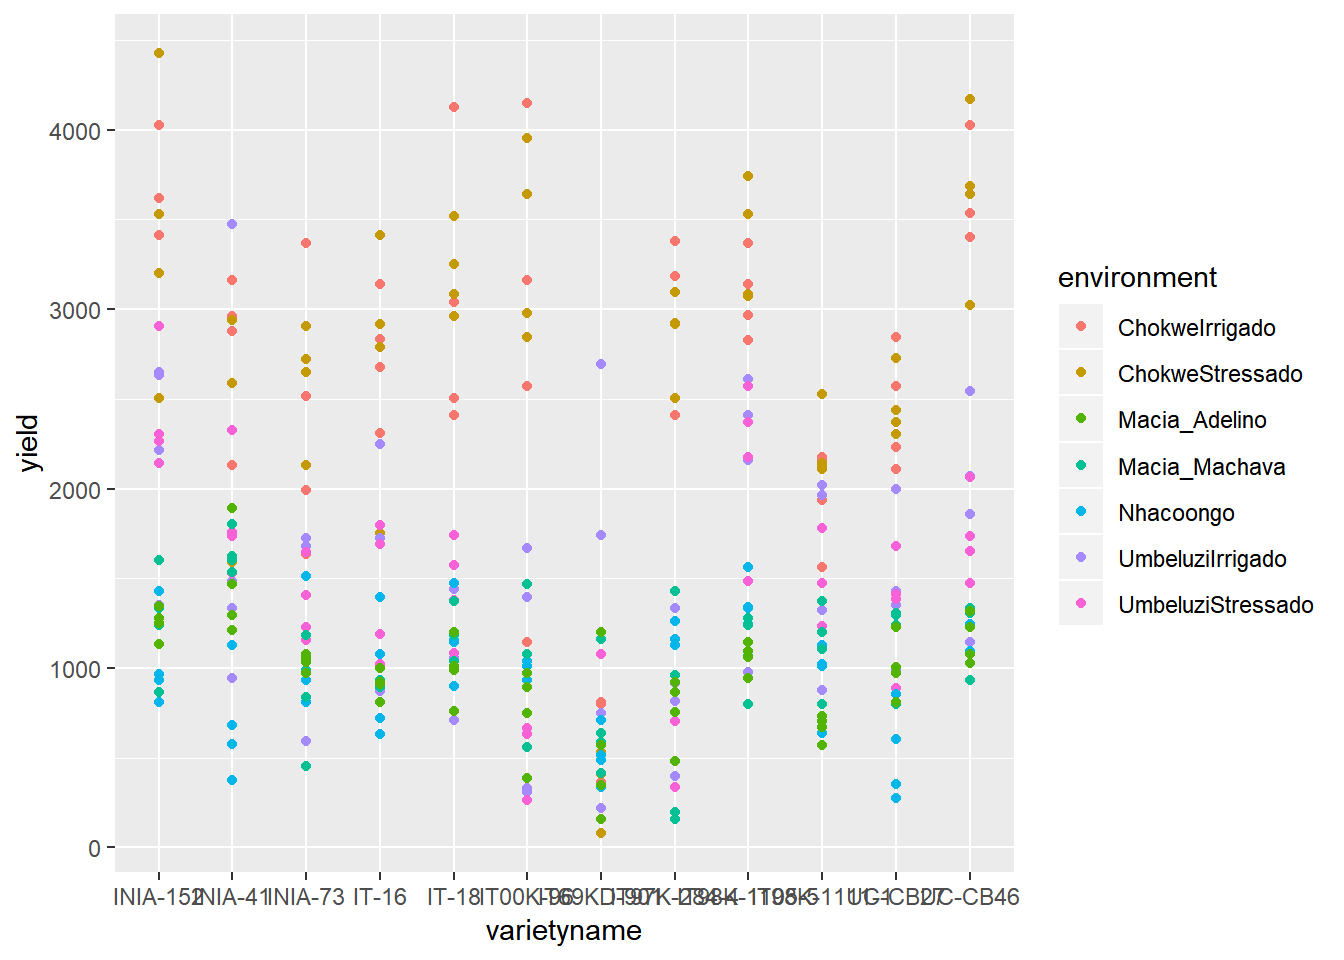
\includegraphics{bookdown-demo_files/figure-latex/unnamed-chunk-149-1.pdf}
We can see from the distribution of striga that there are some farms
with very high levels of striga, and some farms with no striga. The big
range of values makes it hard to make interpretations from this plot, so
taking a square root transformation may help to visualise the
relationship. A log transformation will not help here because of the
large number of 0 values of striga.

\begin{Shaded}
\begin{Highlighting}[]
\KeywordTok{ggplot}\NormalTok{(}\DataTypeTok{data=}\NormalTok{vartrial,}\KeywordTok{aes}\NormalTok{(}\DataTypeTok{y=}\NormalTok{yield,}\DataTypeTok{x=}\NormalTok{environment,}\DataTypeTok{colour=}\NormalTok{varietyname,}\DataTypeTok{group=}\NormalTok{varietyname)) }\OperatorTok{+}
\StringTok{  }\KeywordTok{stat_summary}\NormalTok{(}\DataTypeTok{geom=}\StringTok{"line"}\NormalTok{)}
\end{Highlighting}
\end{Shaded}

\begin{verbatim}
## No summary function supplied, defaulting to `mean_se()
\end{verbatim}

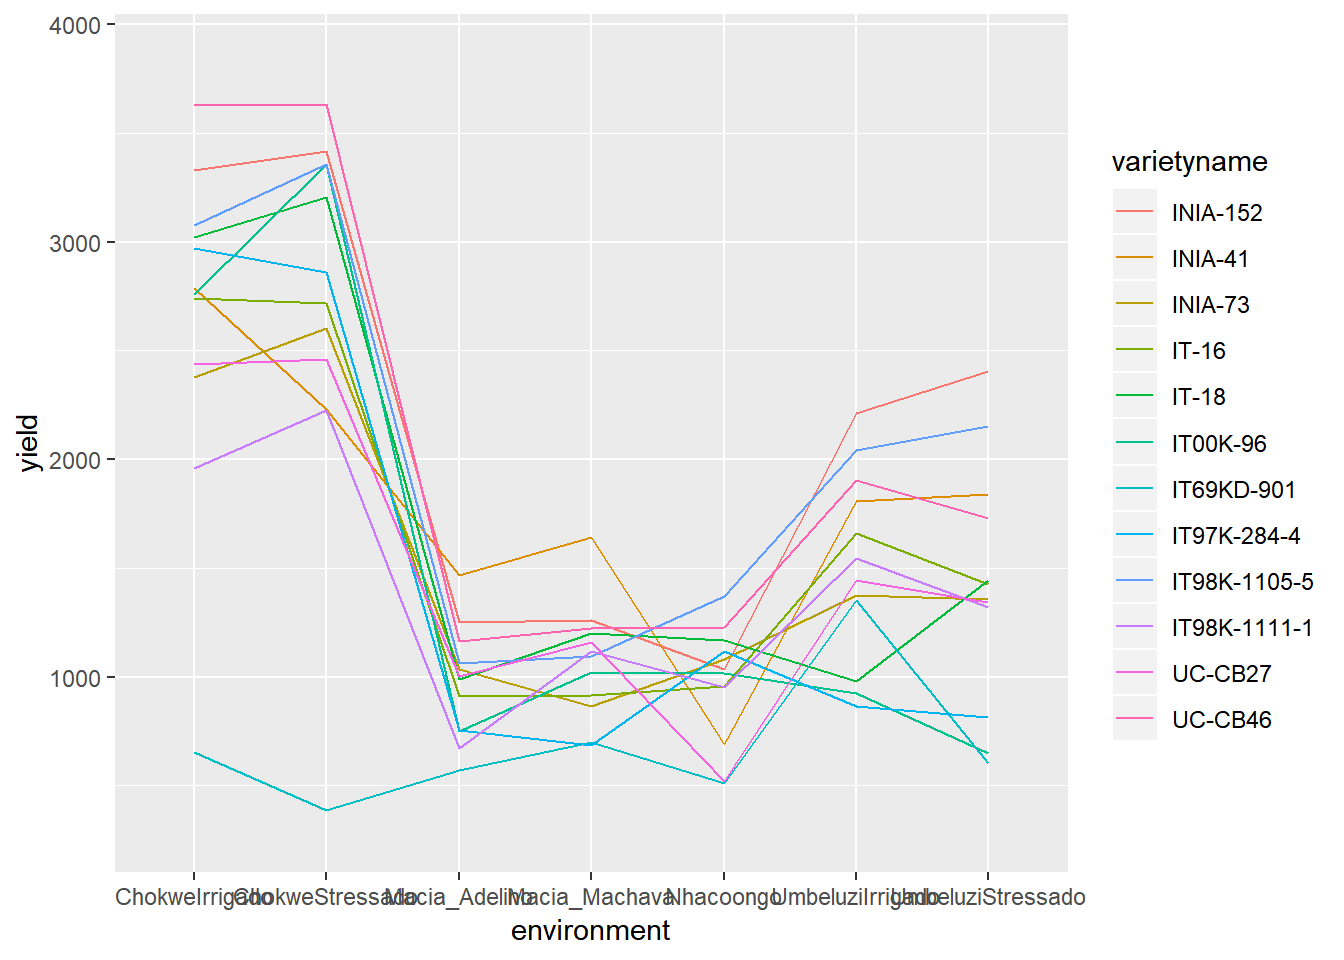
\includegraphics{bookdown-demo_files/figure-latex/unnamed-chunk-150-1.pdf}

\begin{Shaded}
\begin{Highlighting}[]
\KeywordTok{ggplot}\NormalTok{(}\DataTypeTok{data=}\NormalTok{vartrial,}\KeywordTok{aes}\NormalTok{(}\DataTypeTok{y=}\NormalTok{yield,}\DataTypeTok{x=}\NormalTok{varietyname))}\OperatorTok{+}
\StringTok{  }\KeywordTok{geom_boxplot}\NormalTok{(}\KeywordTok{aes}\NormalTok{(}\DataTypeTok{colour=}\NormalTok{varietyname))}\OperatorTok{+}\KeywordTok{facet_wrap}\NormalTok{(}\OperatorTok{~}\NormalTok{environment)}
\end{Highlighting}
\end{Shaded}

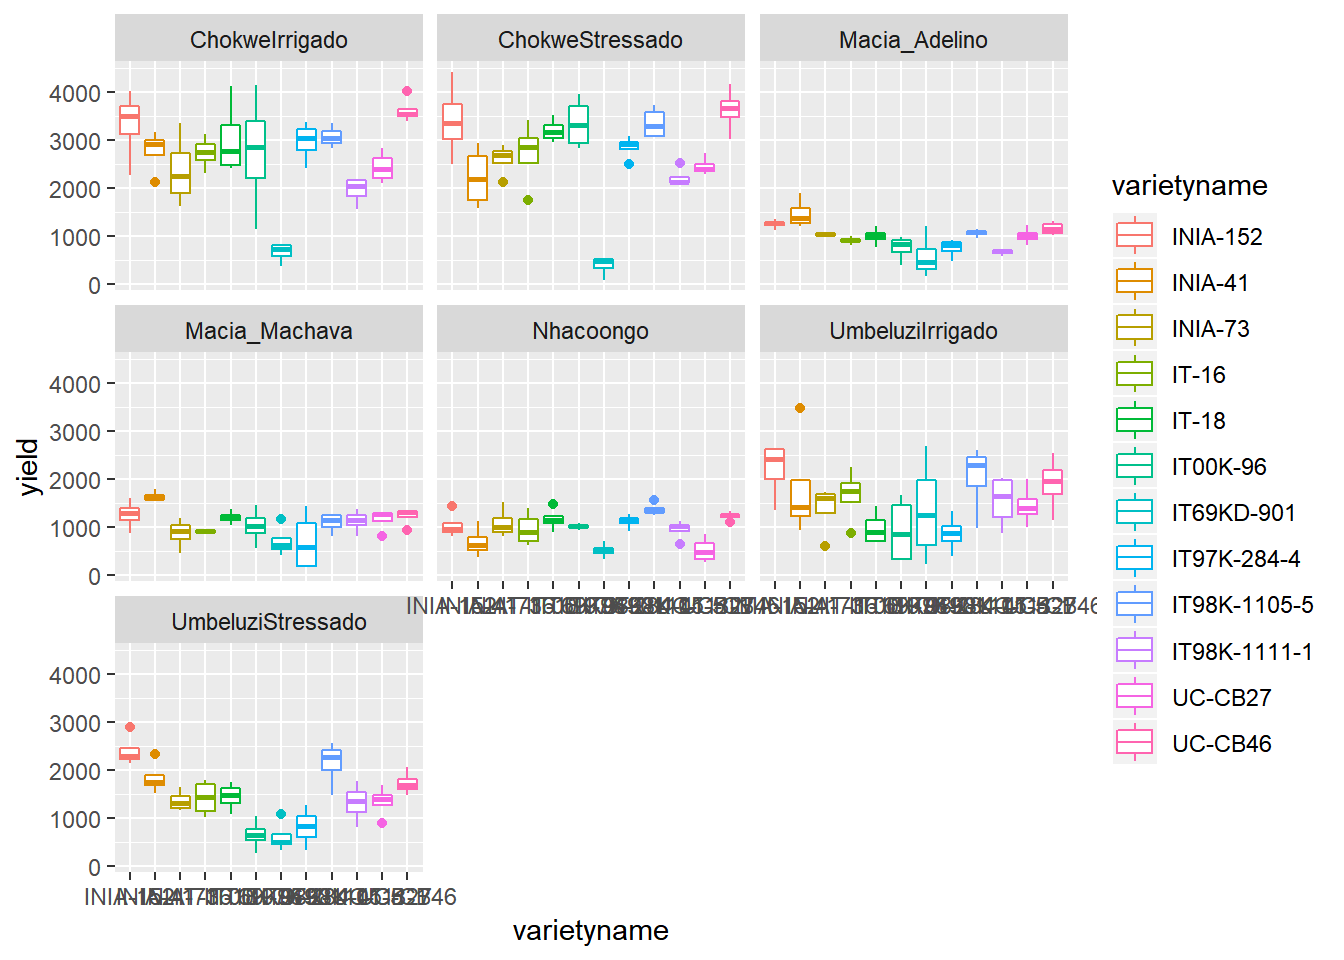
\includegraphics{bookdown-demo_files/figure-latex/unnamed-chunk-151-1.pdf}

\subsubsection{Summary Statistics}\label{summary-statistics-3}

To produce summary statistics, by group, there are many options within
R. One option is to use the summaryBy function, from the doBy library.
The code used for this is quite similar to the code we will use to
produce models in a later step.

\begin{Shaded}
\begin{Highlighting}[]
\KeywordTok{summaryBy}\NormalTok{(yield}\OperatorTok{~}\NormalTok{varietyname}\OperatorTok{+}\NormalTok{environment, }\DataTypeTok{data=}\NormalTok{vartrial, }\DataTypeTok{FUN=}\KeywordTok{c}\NormalTok{(mean,median,sd))}
\end{Highlighting}
\end{Shaded}

\begin{verbatim}
##     varietyname       environment yield.mean yield.median   yield.sd
## 1      INIA-152    ChokweIrrigado   3331.125      3515.55  754.04696
## 2      INIA-152   ChokweStressado   3415.575      3364.45  797.44230
## 3      INIA-152     Macia_Adelino   1253.325      1266.65   89.13744
## 4      INIA-152     Macia_Machava   1260.000      1286.65  303.34677
## 5      INIA-152         Nhacoongo   1035.550       951.10  272.47465
## 6      INIA-152  UmbeluziIrrigado   2211.100      2422.20  607.63851
## 7      INIA-152 UmbeluziStressado   2404.450      2284.45  341.78953
## 8       INIA-41    ChokweIrrigado   2784.425      2920.00  450.29839
## 9       INIA-41   ChokweStressado   2231.100      2195.55  638.69332
## 10      INIA-41     Macia_Adelino   1466.650      1380.00  303.46151
## 11      INIA-41     Macia_Machava   1640.000      1613.35  113.66879
## 12      INIA-41         Nhacoongo    691.100       631.10  319.13814
## 13      INIA-41  UmbeluziIrrigado   1808.875      1408.85 1134.39461
## 14      INIA-41 UmbeluziStressado   1837.775      1746.65  343.30332
## 15      INIA-73    ChokweIrrigado   2377.800      2253.35  753.14137
## 16      INIA-73   ChokweStressado   2602.225      2684.45  330.98096
## 17      INIA-73     Macia_Adelino   1035.550      1044.45   45.33553
## 18      INIA-73     Macia_Machava    866.675       913.35  310.06045
## 19      INIA-73         Nhacoongo   1080.000      1000.00  306.07200
## 20      INIA-73  UmbeluziIrrigado   1377.775      1595.55  529.48470
## 21      INIA-73 UmbeluziStressado   1357.775      1315.55  217.85558
## 22        IT-16    ChokweIrrigado   2740.025      2755.60  344.23188
## 23        IT-16   ChokweStressado   2717.775      2853.35  698.26615
## 24        IT-16     Macia_Adelino    911.100       915.55   76.47932
## 25        IT-16     Macia_Machava    916.650       920.00   19.98891
## 26        IT-16         Nhacoongo    955.575       897.80  350.62212
## 27        IT-16  UmbeluziIrrigado   1660.000      1760.00  574.94960
## 28        IT-16 UmbeluziStressado   1424.450      1440.00  375.91817
## 29        IT-18    ChokweIrrigado   3020.000      2773.35  786.76965
## 30        IT-18   ChokweStressado   3204.425      3168.85  242.29866
## 31        IT-18     Macia_Adelino    991.100      1002.20  180.31386
## 32        IT-18     Macia_Machava   1200.000      1193.35  136.39377
## 33        IT-18         Nhacoongo   1168.925      1151.15  236.80500
## 34        IT-18  UmbeluziIrrigado    980.000       884.45  347.49929
## 35        IT-18 UmbeluziStressado   1444.425      1475.55  282.45094
## 36     IT00K-96    ChokweIrrigado   2757.775      2866.65 1256.70666
## 37     IT00K-96   ChokweStressado   3355.550      3311.10  531.49591
## 38     IT00K-96     Macia_Adelino    751.100       822.20  259.73130
## 39     IT00K-96     Macia_Machava   1020.000      1026.65  372.79207
## 40     IT00K-96         Nhacoongo   1015.550      1026.65   60.48121
## 41     IT00K-96  UmbeluziIrrigado    926.675       862.25  709.53665
## 42     IT00K-96 UmbeluziStressado    651.125       648.90  316.04321
## 43   IT69KD-901    ChokweIrrigado    653.325       720.00  207.66347
## 44   IT69KD-901   ChokweStressado    386.200       466.65  213.00778
## 45   IT69KD-901     Macia_Adelino    568.900       457.80  452.71745
## 46   IT69KD-901     Macia_Machava    700.000       613.35  321.57621
## 47   IT69KD-901         Nhacoongo    513.350       502.25  153.32507
## 48   IT69KD-901  UmbeluziIrrigado   1351.100      1244.45 1094.55845
## 49   IT69KD-901 UmbeluziStressado    604.475       502.25  323.69258
## 50  IT97K-284-4    ChokweIrrigado   2971.125      3048.90  419.96714
## 51  IT97K-284-4   ChokweStressado   2860.000      2920.00  249.32475
## 52  IT97K-284-4     Macia_Adelino    755.575       811.15  196.06625
## 53  IT97K-284-4     Macia_Machava    686.675       580.00  615.51677
## 54  IT97K-284-4         Nhacoongo   1119.975      1146.65  142.04549
## 55  IT97K-284-4  UmbeluziIrrigado    866.675       866.70  383.10437
## 56  IT97K-284-4 UmbeluziStressado    815.550       831.10  392.19694
## 57 IT98K-1105-5    ChokweIrrigado   3075.575      3053.35  233.25939
## 58 IT98K-1105-5   ChokweStressado   3357.775      3306.65  332.37678
## 59 IT98K-1105-5     Macia_Adelino   1062.225      1077.75   84.55315
## 60 IT98K-1105-5     Macia_Machava   1096.675      1153.35  218.37633
## 61 IT98K-1105-5         Nhacoongo   1371.075      1337.75  136.23733
## 62 IT98K-1105-5  UmbeluziIrrigado   2040.000      2284.45  731.99020
## 63 IT98K-1105-5 UmbeluziStressado   2151.100      2275.55  472.27515
## 64 IT98K-1111-1    ChokweIrrigado   1960.000      2048.90  285.44062
## 65 IT98K-1111-1   ChokweStressado   2224.425      2133.30  200.50779
## 66 IT98K-1111-1     Macia_Adelino    671.100       688.90   70.00248
## 67 IT98K-1111-1     Macia_Machava   1120.000      1153.35  240.23445
## 68 IT98K-1111-1         Nhacoongo    951.100      1017.75  213.94711
## 69 IT98K-1111-1  UmbeluziIrrigado   1546.650      1644.40  544.76743
## 70 IT98K-1111-1 UmbeluziStressado   1322.250      1355.60  412.83383
## 71      UC-CB27    ChokweIrrigado   2437.775      2400.00  334.09723
## 72      UC-CB27   ChokweStressado   2460.000      2404.45  187.36800
## 73      UC-CB27     Macia_Adelino   1004.425       988.85  170.19960
## 74      UC-CB27     Macia_Machava   1160.000      1266.65  241.72283
## 75      UC-CB27         Nhacoongo    522.225       480.00  261.37532
## 76      UC-CB27  UmbeluziIrrigado   1444.450      1391.10  415.93051
## 77      UC-CB27 UmbeluziStressado   1342.225      1400.00  329.96221
## 78      UC-CB46    ChokweIrrigado   3626.675      3537.80  273.99739
## 79      UC-CB46   ChokweStressado   3631.100      3666.65  470.28565
## 80      UC-CB46     Macia_Adelino   1163.350      1153.35  134.37868
## 81      UC-CB46     Macia_Machava   1223.325      1313.35  193.65472
## 82      UC-CB46         Nhacoongo   1228.850      1244.40   99.61126
## 83      UC-CB46  UmbeluziIrrigado   1904.450      1964.45  580.47640
## 84      UC-CB46 UmbeluziStressado   1731.100      1693.30  245.60479
\end{verbatim}

\subsection{5. Specify a model for
data}\label{specify-a-model-for-data-4}

In this design, an RCBD, we have one treatment factor, ``treat'', and
one layout factor ``rep''. More information about model fitting can be
found in section 2.

\begin{Shaded}
\begin{Highlighting}[]
\NormalTok{gxemodel1<-}\KeywordTok{lmer}\NormalTok{(yield}\OperatorTok{~}\NormalTok{varietyname}\OperatorTok{*}\NormalTok{environment}\OperatorTok{+}\NormalTok{(}\DecValTok{1}\OperatorTok{|}\NormalTok{rep}\OperatorTok{:}\NormalTok{environment), }\DataTypeTok{data=}\NormalTok{vartrial)}

\NormalTok{gxemodel2<-}\KeywordTok{lmer}\NormalTok{(yield}\OperatorTok{~}\NormalTok{varietyname}\OperatorTok{*}\NormalTok{environment}\OperatorTok{+}\NormalTok{(}\DecValTok{1}\OperatorTok{|}\NormalTok{rep}\OperatorTok{:}\NormalTok{environment)}\OperatorTok{+}\NormalTok{(}\DecValTok{1}\OperatorTok{|}\NormalTok{rep}\OperatorTok{:}\NormalTok{environment}\OperatorTok{:}\NormalTok{row)}\OperatorTok{+}\NormalTok{(}\DecValTok{1}\OperatorTok{|}\NormalTok{rep}\OperatorTok{:}\NormalTok{environment}\OperatorTok{:}\NormalTok{column), }\DataTypeTok{data=}\NormalTok{vartrial)}

\KeywordTok{anova}\NormalTok{(gxemodel2,gxemodel1)}
\end{Highlighting}
\end{Shaded}

\begin{verbatim}
## refitting model(s) with ML (instead of REML)
\end{verbatim}

\begin{verbatim}
## Data: vartrial
## Models:
## gxemodel1: yield ~ varietyname * environment + (1 | rep:environment)
## gxemodel2: yield ~ varietyname * environment + (1 | rep:environment) + (1 | 
## gxemodel2:     rep:environment:row) + (1 | rep:environment:column)
##           Df    AIC    BIC  logLik deviance  Chisq Chi Df Pr(>Chisq)    
## gxemodel1 86 5042.2 5370.5 -2435.1   4870.2                             
## gxemodel2 88 5025.2 5361.1 -2424.6   4849.2 20.977      2  2.785e-05 ***
## ---
## Signif. codes:  0 '***' 0.001 '**' 0.01 '*' 0.05 '.' 0.1 ' ' 1
\end{verbatim}

R is unlike many other software packages in how it fits models. The best
way of handling models in R is to assign the model to a name (in this
case rcbdmodel1) and then ask R to provide different sorts of output for
this model. When you run the above line you will get now output from the
data - this is what we expected to see!

\subsection{6. Check the model}\label{check-the-model-4}

Before interpretting the model any further we should investigate the
model validity, to ensure any conclusions we draw are valid. There are 3
assumptions that we can check for using standard model checking plots.
1. Homogeneity (equal variance) 2. Values with high leverage 3.
Normality of residuals

The function plot() when used with a model will plot the fitted values
from the model against the expected values.

\begin{Shaded}
\begin{Highlighting}[]
\KeywordTok{plot}\NormalTok{(gxemodel2)}
\end{Highlighting}
\end{Shaded}

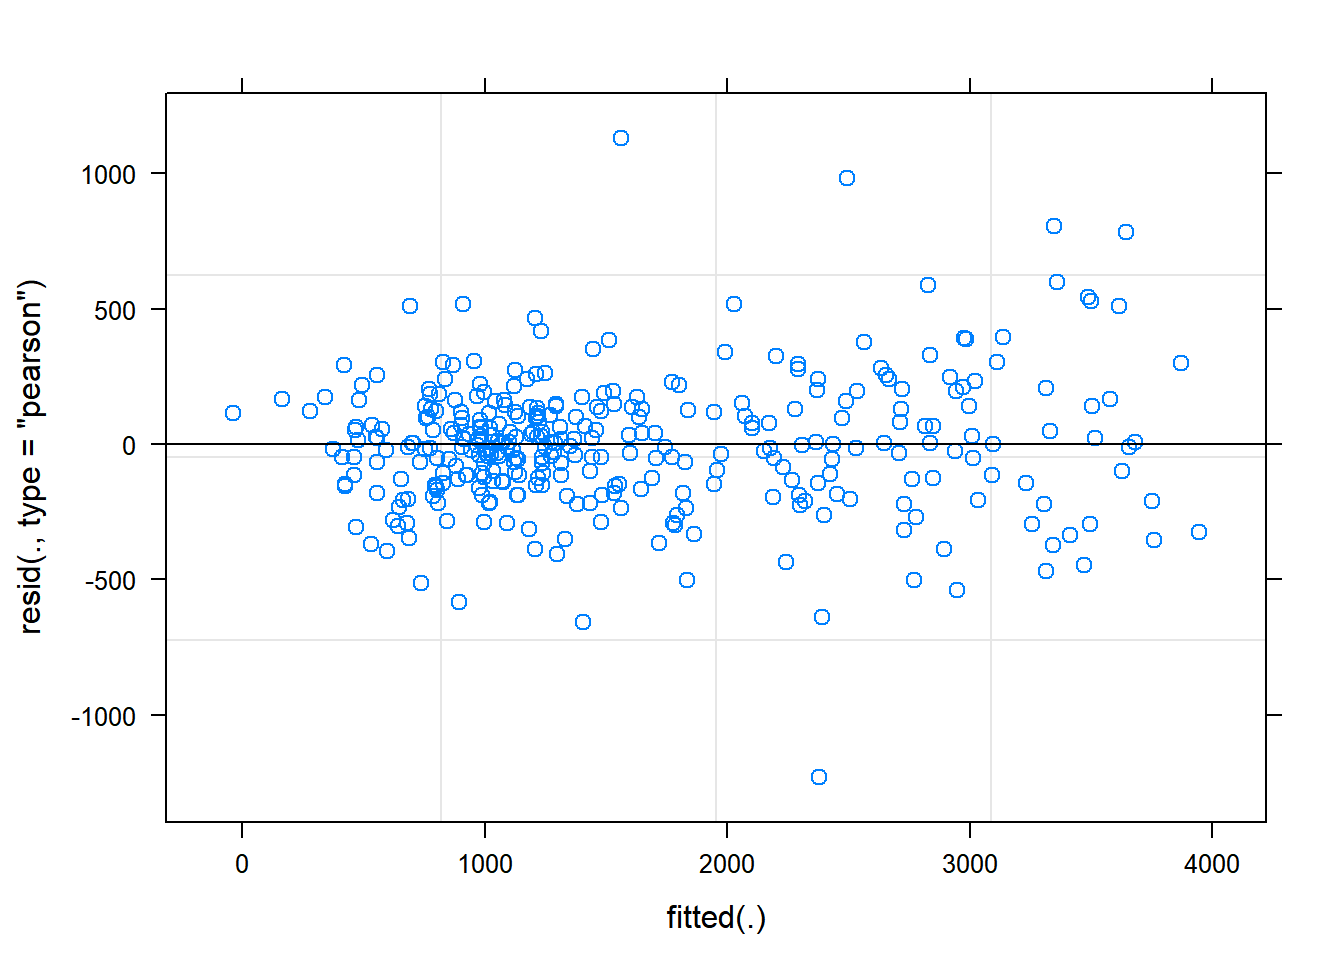
\includegraphics{bookdown-demo_files/figure-latex/unnamed-chunk-154-1.pdf}
The residual Vs fitted plot is a scatter plot of the Residuals on the
y-axis and the fitted on the x-axis and the aim for this plot is to test
the assumption of equal variance of the residuals across the range of
fitted values. Since the residuals do not funnel out (to form
triangular/diamond shape) the assumption of equal variance is met.

We can also see that there are no extreme values in the residuals which
might be potentially causing problems with the validity of our
conclusions (leverage)

To assess the assumption of normality we can produce a qqplot. This
shows us how closely the residuals follow a normal distribution - if
there are severe and syste,matic deviations from the line then we may
want to consider an alternative distribution.

\begin{Shaded}
\begin{Highlighting}[]
\KeywordTok{qqnorm}\NormalTok{(}\KeywordTok{resid}\NormalTok{(gxemodel2))}
\KeywordTok{qqline}\NormalTok{(}\KeywordTok{resid}\NormalTok{(gxemodel2))}
\end{Highlighting}
\end{Shaded}

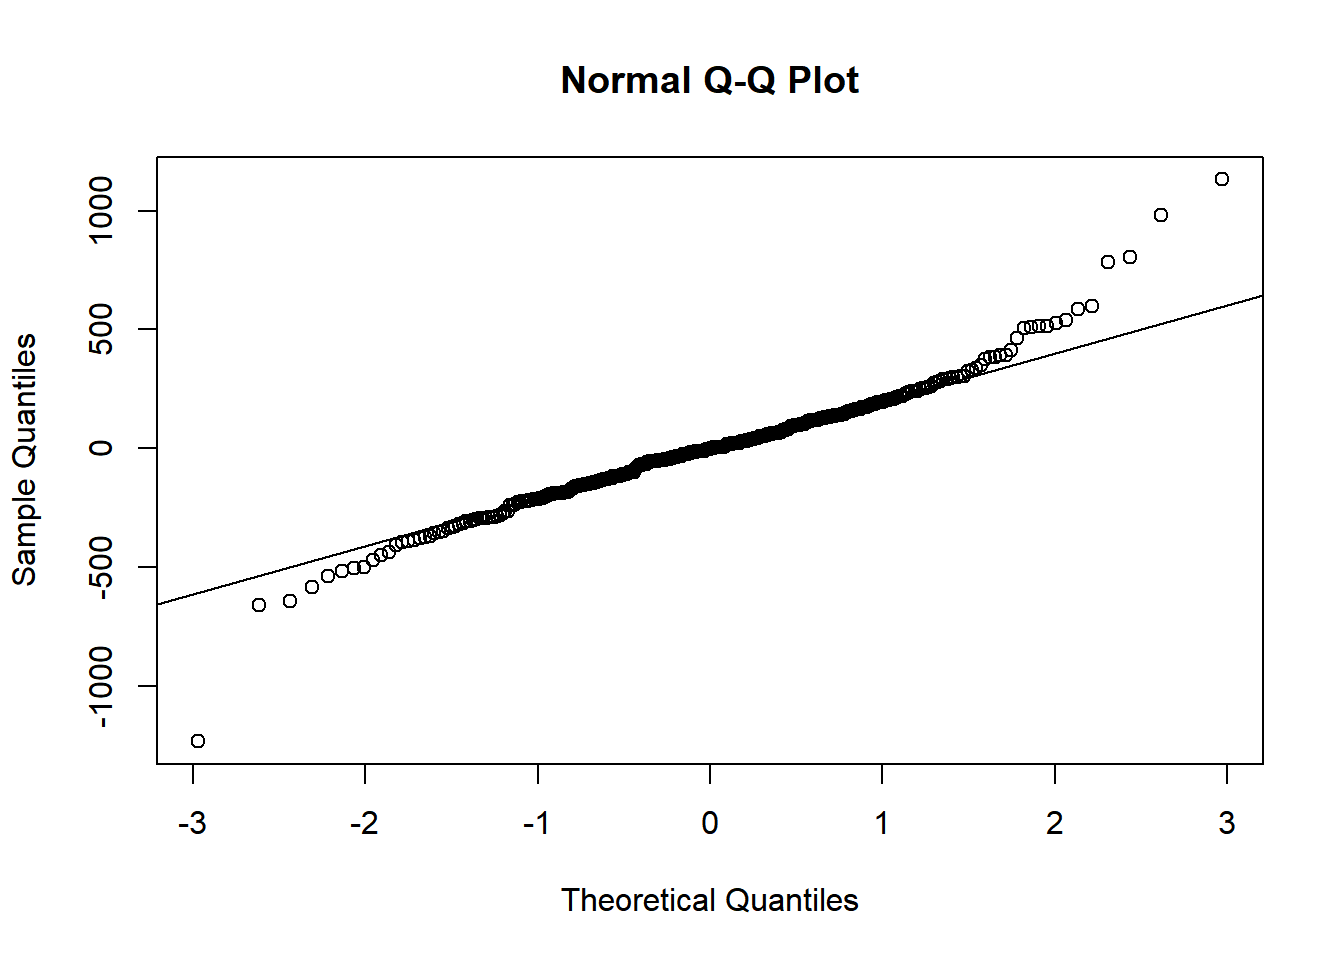
\includegraphics{bookdown-demo_files/figure-latex/unnamed-chunk-155-1.pdf}
In this case the residuals seem to fit the assumption required for
normality.

\subsection{7. Interpret Model}\label{interpret-model-4}

The anova() function only prints the rows of analysis of variance table
for treatment effects when looking at a mixed model fitted using lmer().

\begin{Shaded}
\begin{Highlighting}[]
\KeywordTok{anova}\NormalTok{(gxemodel2, }\DataTypeTok{ddf=}\StringTok{"Kenward-Roger"}\NormalTok{)}
\end{Highlighting}
\end{Shaded}

\begin{verbatim}
## Type III Analysis of Variance Table with Kenward-Roger's method
##                           Sum Sq Mean Sq NumDF  DenDF F value    Pr(>F)
## varietyname             37176902 3379718    11 212.07 33.1312 < 2.2e-16
## environment             20533476 3422246     6  21.00 33.5705 1.038e-09
## varietyname:environment 37168495  563159    66 184.90  5.5128 < 2.2e-16
##                            
## varietyname             ***
## environment             ***
## varietyname:environment ***
## ---
## Signif. codes:  0 '***' 0.001 '**' 0.01 '*' 0.05 '.' 0.1 ' ' 1
\end{verbatim}

ddf=Kenward-Roger tells R which method to use for determining the
calculations of the table; this option matches the defaults found within
SAS or Genstat. The ANOVA table suggests a highly significant effect of
the treatment on the yield.

To obtain the residual variance, and the variance attributed to the
blocks we need an additional command. From these number it is possible
to reconstruct a more classic ANOVA table, if so desired.

\begin{Shaded}
\begin{Highlighting}[]
\KeywordTok{print}\NormalTok{(}\KeywordTok{VarCorr}\NormalTok{(gxemodel2), }\DataTypeTok{comp=}\NormalTok{(}\StringTok{"Variance"}\NormalTok{))}
\end{Highlighting}
\end{Shaded}

\begin{verbatim}
##  Groups                 Name        Variance
##  rep:environment:row    (Intercept)   4500.6
##  rep:environment:column (Intercept)  36719.8
##  rep:environment        (Intercept)  45991.9
##  Residual                           101942.0
\end{verbatim}

\begin{Shaded}
\begin{Highlighting}[]
\KeywordTok{ranova}\NormalTok{(gxemodel2)}
\end{Highlighting}
\end{Shaded}

\begin{verbatim}
## ANOVA-like table for random-effects: Single term deletions
## 
## Model:
## yield ~ varietyname + environment + (1 | rep:environment) + (1 | 
##     rep:environment:row) + (1 | rep:environment:column) + varietyname:environment
##                              npar  logLik    AIC     LRT Df Pr(>Chisq)    
## <none>                         88 -1914.8 4005.5                          
## (1 | rep:environment)          87 -1919.8 4013.6 10.1269  1  0.0014612 ** 
## (1 | rep:environment:row)      87 -1914.9 4003.8  0.2394  1  0.6246201    
## (1 | rep:environment:column)   87 -1920.8 4015.6 12.0793  1  0.0005098 ***
## ---
## Signif. codes:  0 '***' 0.001 '**' 0.01 '*' 0.05 '.' 0.1 ' ' 1
\end{verbatim}

\subsection{8. Present the results from the
model}\label{present-the-results-from-the-model-4}

To help understand what the significant result from the ANOVA table
means we can produce several plots and tables to help us. First we can
use the function emmip() to produce plots of the modelled results,
including 95\% confidence intervals.

\begin{Shaded}
\begin{Highlighting}[]
\KeywordTok{emmip}\NormalTok{(gxemodel2,}\OperatorTok{~}\NormalTok{varietyname}\OperatorTok{|}\NormalTok{environment,}\DataTypeTok{CIs =} \OtherTok{TRUE}\NormalTok{)}
\end{Highlighting}
\end{Shaded}

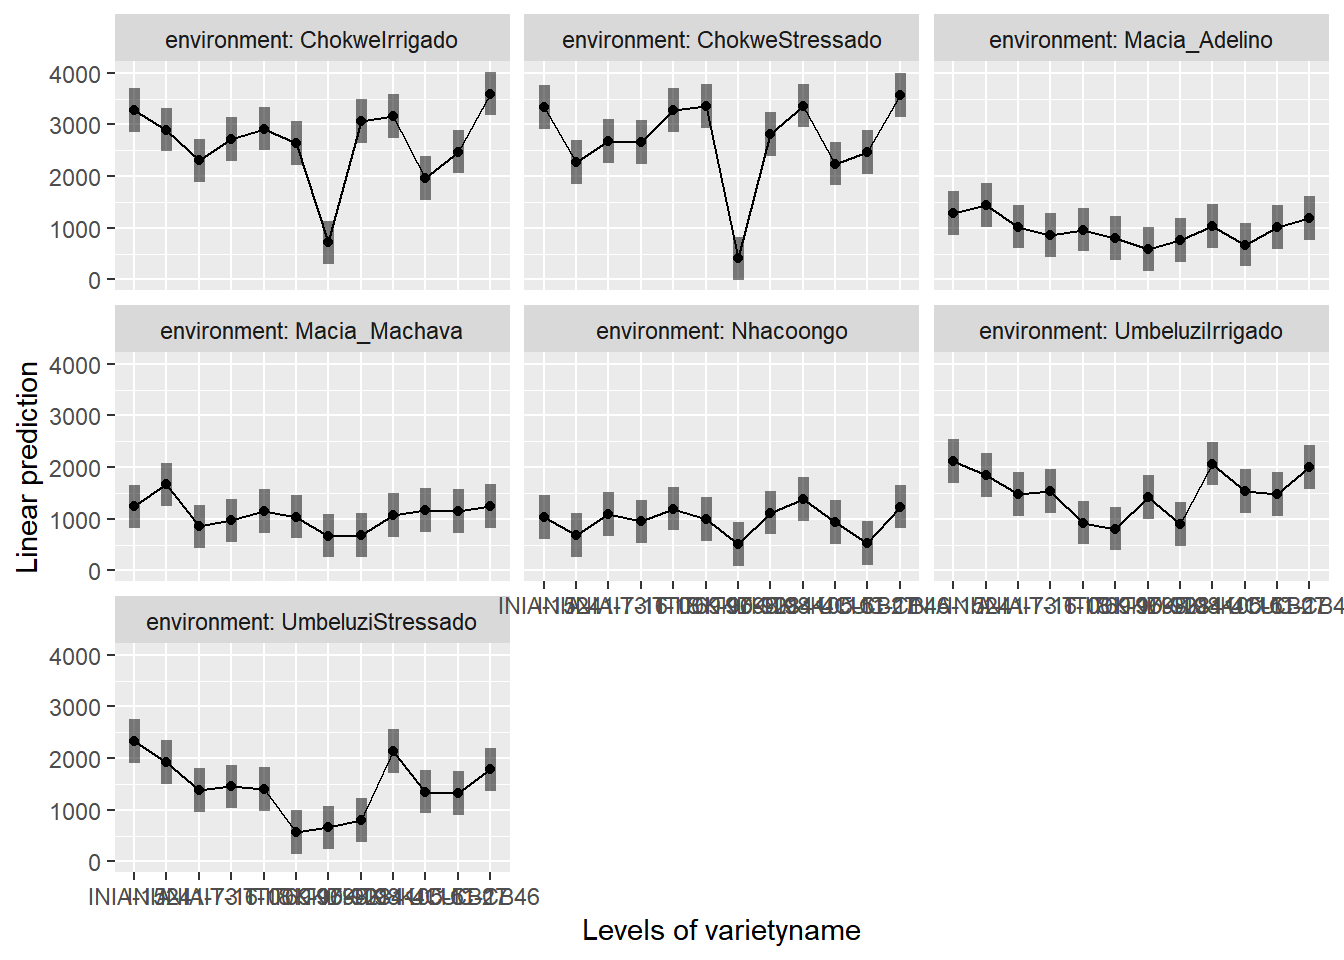
\includegraphics{bookdown-demo_files/figure-latex/unnamed-chunk-158-1.pdf}

Or alternatively

\begin{Shaded}
\begin{Highlighting}[]
\KeywordTok{emmip}\NormalTok{(gxemodel2,}\OperatorTok{~}\NormalTok{varietyname}\OperatorTok{|}\NormalTok{environment,}\DataTypeTok{CIs =} \OtherTok{TRUE}\NormalTok{)}
\end{Highlighting}
\end{Shaded}

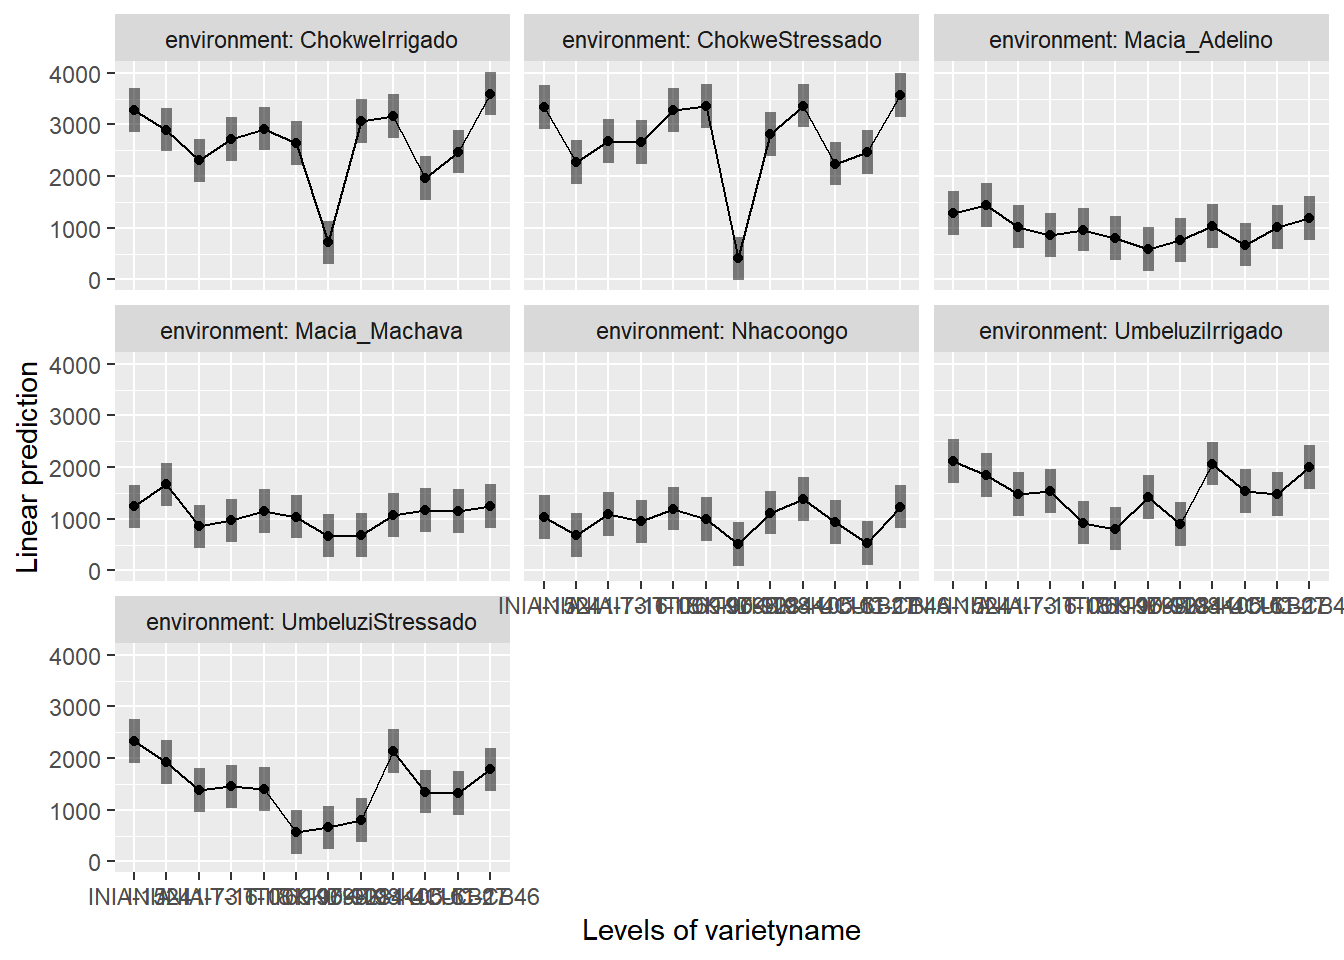
\includegraphics{bookdown-demo_files/figure-latex/unnamed-chunk-159-1.pdf}

\begin{Shaded}
\begin{Highlighting}[]
\KeywordTok{emmip}\NormalTok{(gxemodel2,varietyname}\OperatorTok{~}\NormalTok{environment)}\OperatorTok{+}\KeywordTok{coord_flip}\NormalTok{()}
\end{Highlighting}
\end{Shaded}

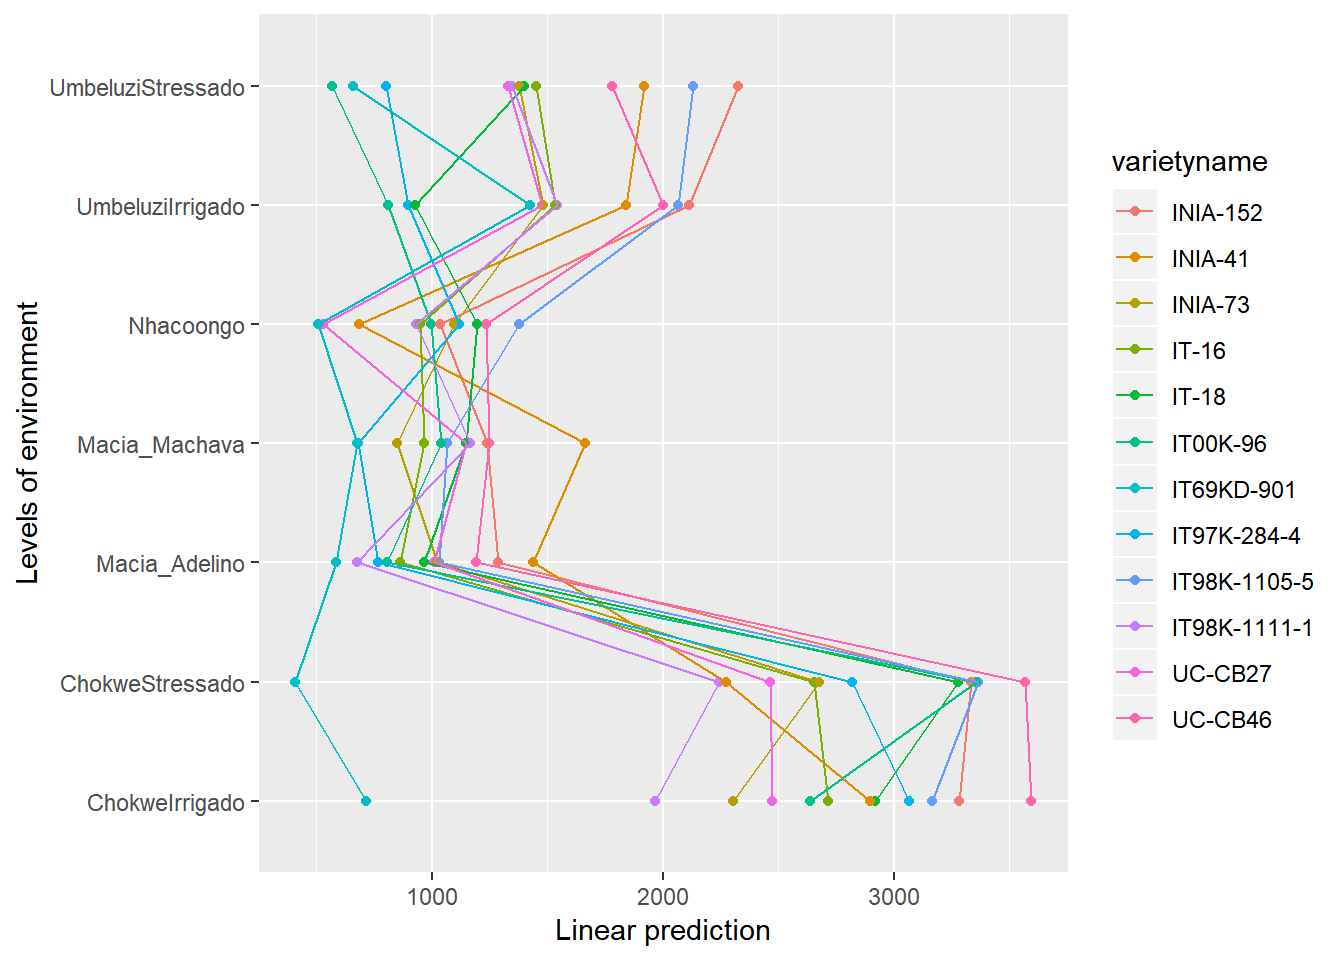
\includegraphics{bookdown-demo_files/figure-latex/unnamed-chunk-159-2.pdf}

To obtain the numbers used in creating this graph we can use the
function emmeans.

\begin{Shaded}
\begin{Highlighting}[]
\KeywordTok{emmeans}\NormalTok{(gxemodel2, }\OperatorTok{~}\NormalTok{varietyname}\OperatorTok{|}\NormalTok{environment)}
\end{Highlighting}
\end{Shaded}

\begin{verbatim}
## environment = ChokweIrrigado:
##  varietyname     emmean       SE     df   lower.CL  upper.CL
##  INIA-152     3281.4112 212.8278 114.96 2859.83867 3702.9837
##  INIA-41      2897.8775 212.3522 113.73 2477.19888 3318.5562
##  INIA-73      2303.3229 213.5745 116.18 1880.31855 2726.3273
##  IT-16        2714.7860 213.4026 115.99 2292.11494 3137.4571
##  IT-18        2918.8710 212.7347 114.70 2497.47295 3340.2690
##  IT00K-96     2635.6529 213.4856 116.25 2212.82719 3058.4786
##  IT69KD-901    714.9043 213.2427 115.33  292.52460 1137.2840
##  IT97K-284-4  3066.1619 214.0881 117.31 2642.18359 3490.1402
##  IT98K-1105-5 3166.2457 212.7774 114.03 2744.73650 3587.7549
##  IT98K-1111-1 1968.2274 213.8460 117.32 1544.72864 2391.7262
##  UC-CB27      2473.2456 213.3913 115.72 2050.58653 2895.9046
##  UC-CB46      3594.9186 212.7865 114.45 3173.40803 4016.4291
## 
## environment = ChokweStressado:
##  varietyname     emmean       SE     df   lower.CL  upper.CL
##  INIA-152     3334.8789 212.7797 115.10 2913.40717 3756.3507
##  INIA-41      2275.2091 212.8143 114.74 1853.65490 2696.7634
##  INIA-73      2678.5428 212.7546 114.72 2257.10603 3099.9796
##  IT-16        2653.7807 213.7745 116.82 2230.40488 3077.1566
##  IT-18        3278.5687 213.1497 115.45 2856.37770 3700.7596
##  IT00K-96     3356.0290 212.3933 113.73 2935.26899 3776.7891
##  IT69KD-901    408.5862 212.4452 114.14  -12.26047  829.4328
##  IT97K-284-4  2818.0288 213.5762 116.35 2395.02778 3241.0299
##  IT98K-1105-5 3365.5194 213.2964 115.80 2943.05141 3787.9874
##  IT98K-1111-1 2243.5917 213.8507 116.61 1820.05673 2667.1267
##  UC-CB27      2464.3505 213.2879 115.95 2041.90479 2886.7962
##  UC-CB46      3569.0641 213.3254 115.68 3146.53401 3991.5941
## 
## environment = Macia_Adelino:
##  varietyname     emmean       SE     df   lower.CL  upper.CL
##  INIA-152     1284.9275 213.4738 116.33  862.12853 1707.7265
##  INIA-41      1438.7231 213.5401 116.02 1015.78093 1861.6653
##  INIA-73      1020.4183 212.7172 114.25  599.03700 1441.7996
##  IT-16         862.7489 213.2524 115.43  440.35378 1285.1440
##  IT-18         965.1424 212.7224 114.26  543.75121 1386.5335
##  IT00K-96      807.3334 213.7587 116.26  383.96731 1230.6995
##  IT69KD-901    585.0126 212.7661 114.94  163.56158 1006.4636
##  IT97K-284-4   765.4647 213.0184 115.20  343.52395 1187.4054
##  IT98K-1105-5 1029.6298 212.9650 115.19  607.79455 1451.4650
##  IT98K-1111-1  674.6159 213.4223 116.51  251.92560 1097.3063
##  UC-CB27      1011.1723 213.0471 114.83  589.16026 1433.1844
##  UC-CB46      1190.5311 213.4851 115.80  767.68915 1613.3730
## 
## environment = Macia_Machava:
##  varietyname     emmean       SE     df   lower.CL  upper.CL
##  INIA-152     1239.1098 213.7555 116.53  815.76018 1662.4593
##  INIA-41      1663.7967 213.0438 115.98 1241.83586 2085.7575
##  INIA-73       850.2913 213.5306 116.23  427.37579 1273.2069
##  IT-16         967.4732 212.9415 114.59  545.66093 1389.2855
##  IT-18        1148.5561 213.4814 115.88  725.72450 1571.3877
##  IT00K-96     1040.3047 212.9071 114.73  618.56630 1462.0431
##  IT69KD-901    674.8924 213.3063 115.59  252.39644 1097.3884
##  IT97K-284-4   680.9149 212.3123 114.12  260.33064 1101.4992
##  IT98K-1105-5 1067.2538 212.8659 115.40  645.62284 1488.8848
##  IT98K-1111-1 1164.8208 213.6071 116.73  741.77309 1587.8685
##  UC-CB27      1146.1091 213.5501 116.75  723.17485 1569.0434
##  UC-CB46      1246.4771 213.2155 115.18  824.14537 1668.8089
## 
## environment = Nhacoongo:
##  varietyname     emmean       SE     df   lower.CL  upper.CL
##  INIA-152     1035.3705 213.7555 116.53  612.02091 1458.7201
##  INIA-41       683.1821 213.0438 115.98  261.22132 1105.1429
##  INIA-73      1093.8123 213.5306 116.23  670.89675 1516.7278
##  IT-16         949.0727 212.9415 114.59  527.26042 1370.8850
##  IT-18        1196.2705 213.4814 115.88  773.43886 1619.1021
##  IT00K-96      995.8209 212.9071 114.73  574.08247 1417.5593
##  IT69KD-901    506.8616 213.3063 115.59   84.36557  929.3576
##  IT97K-284-4  1118.8071 212.3123 114.12  698.22285 1539.3914
##  IT98K-1105-5 1377.8540 212.8659 115.40  956.22305 1799.4850
##  IT98K-1111-1  930.7708 213.6071 116.73  507.72304 1353.8185
##  UC-CB27       529.4971 213.5501 116.75  106.56281  952.4313
##  UC-CB46      1235.9555 213.2155 115.18  813.62372 1658.2873
## 
## environment = UmbeluziIrrigado:
##  varietyname     emmean       SE     df   lower.CL  upper.CL
##  INIA-152     2112.2016 213.3949 115.85 1689.54033 2534.8628
##  INIA-41      1842.2548 212.8510 115.20 1420.64580 2263.8638
##  INIA-73      1483.0058 212.9097 115.41 1061.28887 1904.7228
##  IT-16        1535.3689 213.6885 116.60 1112.15478 1958.5830
##  IT-18         927.1970 213.1870 115.02  504.91536 1349.4787
##  IT00K-96      810.6883 212.7889 114.99  389.19411 1232.1825
##  IT69KD-901   1424.4582 213.3224 115.55 1001.92884 1846.9875
##  IT97K-284-4   895.8138 212.9352 114.80  474.02221 1317.6055
##  IT98K-1105-5 2065.8614 212.8188 114.89 1644.30415 2487.4187
##  IT98K-1111-1 1542.8659 213.1575 115.62 1120.66581 1965.0659
##  UC-CB27      1475.3602 212.9806 114.65 1053.47306 1897.2474
##  UC-CB46      2002.6740 212.6761 115.11 1581.40786 2423.9402
## 
## environment = UmbeluziStressado:
##  varietyname     emmean       SE     df   lower.CL  upper.CL
##  INIA-152     2327.3996 213.0239 115.54 1905.46145 2749.3378
##  INIA-41      1919.5881 212.9661 115.41 1497.75935 2341.4169
##  INIA-73      1377.4359 213.6416 116.23  954.30071 1800.5712
##  IT-16        1450.3158 213.9875 117.16 1026.53077 1874.1008
##  IT-18        1400.5776 213.3006 116.21  978.11710 1823.0381
##  IT00K-96      565.3932 213.0577 115.40  143.38258  987.4039
##  IT69KD-901    657.5039 213.4439 115.55  234.73427 1080.2736
##  IT97K-284-4   801.4592 213.1804 115.54  379.21080 1223.7075
##  IT98K-1105-5 2130.4133 213.4059 115.47 1707.71546 2553.1112
##  IT98K-1111-1 1348.3902 212.6457 114.08  927.14379 1769.6366
##  UC-CB27      1328.3779 213.3563 115.76  905.78983 1750.9660
##  UC-CB46      1779.8452 213.5101 115.89 1356.95749 2202.7329
## 
## Degrees-of-freedom method: kenward-roger 
## Confidence level used: 0.95
\end{verbatim}

And one method for conducting mean separation analysis, holding striga
effect constant, we can use the function cld().

\begin{Shaded}
\begin{Highlighting}[]
\KeywordTok{cld}\NormalTok{(}\KeywordTok{emmeans}\NormalTok{(gxemodel2, }\OperatorTok{~}\NormalTok{varietyname}\OperatorTok{*}\NormalTok{environment))}
\end{Highlighting}
\end{Shaded}

\begin{verbatim}
##  varietyname  environment          emmean       SE     df   lower.CL
##  IT69KD-901   ChokweStressado    408.5862 212.4452 114.14  -12.26047
##  IT69KD-901   Nhacoongo          506.8616 213.3063 115.59   84.36557
##  UC-CB27      Nhacoongo          529.4971 213.5501 116.75  106.56281
##  IT00K-96     UmbeluziStressado  565.3932 213.0577 115.40  143.38258
##  IT69KD-901   Macia_Adelino      585.0126 212.7661 114.94  163.56158
##  IT69KD-901   UmbeluziStressado  657.5039 213.4439 115.55  234.73427
##  IT98K-1111-1 Macia_Adelino      674.6159 213.4223 116.51  251.92560
##  IT69KD-901   Macia_Machava      674.8924 213.3063 115.59  252.39644
##  IT97K-284-4  Macia_Machava      680.9149 212.3123 114.12  260.33064
##  INIA-41      Nhacoongo          683.1821 213.0438 115.98  261.22132
##  IT69KD-901   ChokweIrrigado     714.9043 213.2427 115.33  292.52460
##  IT97K-284-4  Macia_Adelino      765.4647 213.0184 115.20  343.52395
##  IT97K-284-4  UmbeluziStressado  801.4592 213.1804 115.54  379.21080
##  IT00K-96     Macia_Adelino      807.3334 213.7587 116.26  383.96731
##  IT00K-96     UmbeluziIrrigado   810.6883 212.7889 114.99  389.19411
##  INIA-73      Macia_Machava      850.2913 213.5306 116.23  427.37579
##  IT-16        Macia_Adelino      862.7489 213.2524 115.43  440.35378
##  IT97K-284-4  UmbeluziIrrigado   895.8138 212.9352 114.80  474.02221
##  IT-18        UmbeluziIrrigado   927.1970 213.1870 115.02  504.91536
##  IT98K-1111-1 Nhacoongo          930.7708 213.6071 116.73  507.72304
##  IT-16        Nhacoongo          949.0727 212.9415 114.59  527.26042
##  IT-18        Macia_Adelino      965.1424 212.7224 114.26  543.75121
##  IT-16        Macia_Machava      967.4732 212.9415 114.59  545.66093
##  IT00K-96     Nhacoongo          995.8209 212.9071 114.73  574.08247
##  UC-CB27      Macia_Adelino     1011.1723 213.0471 114.83  589.16026
##  INIA-73      Macia_Adelino     1020.4183 212.7172 114.25  599.03700
##  IT98K-1105-5 Macia_Adelino     1029.6298 212.9650 115.19  607.79455
##  INIA-152     Nhacoongo         1035.3705 213.7555 116.53  612.02091
##  IT00K-96     Macia_Machava     1040.3047 212.9071 114.73  618.56630
##  IT98K-1105-5 Macia_Machava     1067.2538 212.8659 115.40  645.62284
##  INIA-73      Nhacoongo         1093.8123 213.5306 116.23  670.89675
##  IT97K-284-4  Nhacoongo         1118.8071 212.3123 114.12  698.22285
##  UC-CB27      Macia_Machava     1146.1091 213.5501 116.75  723.17485
##  IT-18        Macia_Machava     1148.5561 213.4814 115.88  725.72450
##  IT98K-1111-1 Macia_Machava     1164.8208 213.6071 116.73  741.77309
##  UC-CB46      Macia_Adelino     1190.5311 213.4851 115.80  767.68915
##  IT-18        Nhacoongo         1196.2705 213.4814 115.88  773.43886
##  UC-CB46      Nhacoongo         1235.9555 213.2155 115.18  813.62372
##  INIA-152     Macia_Machava     1239.1098 213.7555 116.53  815.76018
##  UC-CB46      Macia_Machava     1246.4771 213.2155 115.18  824.14537
##  INIA-152     Macia_Adelino     1284.9275 213.4738 116.33  862.12853
##  UC-CB27      UmbeluziStressado 1328.3779 213.3563 115.76  905.78983
##  IT98K-1111-1 UmbeluziStressado 1348.3902 212.6457 114.08  927.14379
##  INIA-73      UmbeluziStressado 1377.4359 213.6416 116.23  954.30071
##  IT98K-1105-5 Nhacoongo         1377.8540 212.8659 115.40  956.22305
##  IT-18        UmbeluziStressado 1400.5776 213.3006 116.21  978.11710
##  IT69KD-901   UmbeluziIrrigado  1424.4582 213.3224 115.55 1001.92884
##  INIA-41      Macia_Adelino     1438.7231 213.5401 116.02 1015.78093
##  IT-16        UmbeluziStressado 1450.3158 213.9875 117.16 1026.53077
##  UC-CB27      UmbeluziIrrigado  1475.3602 212.9806 114.65 1053.47306
##  INIA-73      UmbeluziIrrigado  1483.0058 212.9097 115.41 1061.28887
##  IT-16        UmbeluziIrrigado  1535.3689 213.6885 116.60 1112.15478
##  IT98K-1111-1 UmbeluziIrrigado  1542.8659 213.1575 115.62 1120.66581
##  INIA-41      Macia_Machava     1663.7967 213.0438 115.98 1241.83586
##  UC-CB46      UmbeluziStressado 1779.8452 213.5101 115.89 1356.95749
##  INIA-41      UmbeluziIrrigado  1842.2548 212.8510 115.20 1420.64580
##  INIA-41      UmbeluziStressado 1919.5881 212.9661 115.41 1497.75935
##  IT98K-1111-1 ChokweIrrigado    1968.2274 213.8460 117.32 1544.72864
##  UC-CB46      UmbeluziIrrigado  2002.6740 212.6761 115.11 1581.40786
##  IT98K-1105-5 UmbeluziIrrigado  2065.8614 212.8188 114.89 1644.30415
##  INIA-152     UmbeluziIrrigado  2112.2016 213.3949 115.85 1689.54033
##  IT98K-1105-5 UmbeluziStressado 2130.4133 213.4059 115.47 1707.71546
##  IT98K-1111-1 ChokweStressado   2243.5917 213.8507 116.61 1820.05673
##  INIA-41      ChokweStressado   2275.2091 212.8143 114.74 1853.65490
##  INIA-73      ChokweIrrigado    2303.3229 213.5745 116.18 1880.31855
##  INIA-152     UmbeluziStressado 2327.3996 213.0239 115.54 1905.46145
##  UC-CB27      ChokweStressado   2464.3505 213.2879 115.95 2041.90479
##  UC-CB27      ChokweIrrigado    2473.2456 213.3913 115.72 2050.58653
##  IT00K-96     ChokweIrrigado    2635.6529 213.4856 116.25 2212.82719
##  IT-16        ChokweStressado   2653.7807 213.7745 116.82 2230.40488
##  INIA-73      ChokweStressado   2678.5428 212.7546 114.72 2257.10603
##  IT-16        ChokweIrrigado    2714.7860 213.4026 115.99 2292.11494
##  IT97K-284-4  ChokweStressado   2818.0288 213.5762 116.35 2395.02778
##  INIA-41      ChokweIrrigado    2897.8775 212.3522 113.73 2477.19888
##  IT-18        ChokweIrrigado    2918.8710 212.7347 114.70 2497.47295
##  IT97K-284-4  ChokweIrrigado    3066.1619 214.0881 117.31 2642.18359
##  IT98K-1105-5 ChokweIrrigado    3166.2457 212.7774 114.03 2744.73650
##  IT-18        ChokweStressado   3278.5687 213.1497 115.45 2856.37770
##  INIA-152     ChokweIrrigado    3281.4112 212.8278 114.96 2859.83867
##  INIA-152     ChokweStressado   3334.8789 212.7797 115.10 2913.40717
##  IT00K-96     ChokweStressado   3356.0290 212.3933 113.73 2935.26899
##  IT98K-1105-5 ChokweStressado   3365.5194 213.2964 115.80 2943.05141
##  UC-CB46      ChokweStressado   3569.0641 213.3254 115.68 3146.53401
##  UC-CB46      ChokweIrrigado    3594.9186 212.7865 114.45 3173.40803
##   upper.CL .group                                
##   829.4328  1                                    
##   929.3576  12                                   
##   952.4313  1234                                 
##   987.4039  1 3                                  
##  1006.4636  1234                                 
##  1080.2736  1 3 5                                
##  1097.3063  12345678                             
##  1097.3884  12345678                             
##  1101.4992  12345678                             
##  1105.1429  12345678                             
##  1137.2840  1234 6  90                           
##  1187.4054  1234567890AB                         
##  1223.7075  12345 7 9 A C                        
##  1230.6995  1234567890ABCD                       
##  1232.1825  12345678                             
##  1273.2069  1234567890ABCDEF                     
##  1285.1440  1234567890ABCDEF                     
##  1317.6055  12345678      E                      
##  1349.4787  12345678      E                      
##  1353.8185  1234567890ABCDEFG                    
##  1370.8850  1234567890ABCDEFG                    
##  1386.5335  1234567890ABCDEFGH                   
##  1389.2855  1234567890ABCDEFGH                   
##  1417.5593  1234567890ABCDEFGHI                  
##  1433.1844  1234567890ABCDEFGHI                  
##  1441.7996  1234567890ABCDEFGHIJ                 
##  1451.4650  1234567890ABCDEFGHIJ                 
##  1458.7201  1234567890ABCDEFGHIJ                 
##  1462.0431  1234567890ABCDEFGHIJ                 
##  1488.8848  1234567890ABCDEFGHIJ                 
##  1516.7278  1234567890ABCDEFGHIJ                 
##  1539.3914  1234567890ABCDEFGHIJ                 
##  1569.0434  1234567890ABCDEFGHIJ                 
##  1571.3877  1234567890ABCDEFGHIJ                 
##  1587.8685  1234567890ABCDEFGHIJK                
##  1613.3730  1234567890ABCDEFGHIJK                
##  1619.1021  1234567890ABCDEFGHIJK                
##  1658.2873  1234567890ABCDEFGHIJK                
##  1662.4593  1234567890ABCDEFGHIJK                
##  1668.8089  1234567890ABCDEFGHIJK                
##  1707.7265  1234567890ABCDEFGHIJK                
##  1750.9660  1234567890ABCDEFGHIJKL               
##  1769.6366  1234567890ABCDEFGHIJKLM              
##  1800.5712  1234567890ABCDEFGHIJKLMN             
##  1799.4850  1234567890ABCDEFGHIJKLMN             
##  1823.0381  1234567890ABCDEFGHIJKLMNO            
##  1846.9875  1234567890ABCDEFGHIJKLMNO            
##  1861.6653  1234567890ABCDEFGHIJKLMNO            
##  1874.1008  1234567890ABCDEFGHIJKLMNO            
##  1897.2474  1234567890ABCDEFGHIJKLMNO            
##  1904.7228  1234567890ABCDEFGHIJKLMNO            
##  1958.5830  1234567890ABCDEFGHIJKLMNOP           
##  1965.0659  1234567890ABCDEFGHIJKLMNOP           
##  2085.7575  1234567890ABCDEFGHIJKLMNOPQ          
##  2202.7329   2 4 67890ABCDEFGHIJKLMNOPQR         
##  2263.8638    34567890ABCDEFGHIJKLMNOPQR         
##  2341.4169       6 8 0 B DEFGHIJKLMNOPQRS        
##  2391.7262      5 78  ABCDEFGHIJKLMNOPQR T       
##  2423.9402          90ABCD FGHIJKLMNOPQRSTU      
##  2487.4187            ABCD FGHIJKLMNOPQRSTUVWX   
##  2534.8628              CD FGHIJKLMNOPQRSTUVWX   
##  2553.1112                EFGHIJKLMNOPQRSTUVWX   
##  2667.1267                  GHIJKLMNOPQRSTUV     
##  2696.7634                   HIJKLMNOPQRSTU W    
##  2726.3273                    IJKLMNOPQRSTUVWXY  
##  2749.3378                     JKLMNOPQRSTUVWXYZa
##  2886.7962                      KLMNOPQRSTUVWX Z 
##  2895.9046                      KLMNOPQRSTUVWXY  
##  3058.4786                       LMNOPQRSTUVWXYZa
##  3077.1566                        MNOPQRSTUVWXYZa
##  3099.9796                         NOPQRSTUVWXYZa
##  3137.4571                          OPQRSTUVWXYZa
##  3241.0299                           PQRSTUVWXYZa
##  3318.5562                            QRSTUVWXYZa
##  3340.2690                            QRSTUVWXYZa
##  3490.1402                             RSTUVWXYZa
##  3587.7549                              S UVWXYZa
##  3700.7596                               TUVWXYZa
##  3702.9837                                UVWXYZa
##  3756.3507                                 V XYZa
##  3776.7891                                   XYZa
##  3787.9874                                  WXYZa
##  3991.5941                                    Y a
##  4016.4291                                     Za
## 
## Degrees-of-freedom method: kenward-roger 
## Confidence level used: 0.95 
## P value adjustment: tukey method for comparing a family of 84 estimates 
## significance level used: alpha = 0.05
\end{verbatim}

\begin{Shaded}
\begin{Highlighting}[]
\KeywordTok{cld}\NormalTok{(}\KeywordTok{emmeans}\NormalTok{(gxemodel2, }\OperatorTok{~}\NormalTok{varietyname}\OperatorTok{|}\NormalTok{environment))}
\end{Highlighting}
\end{Shaded}

\begin{verbatim}
## environment = ChokweIrrigado:
##  varietyname     emmean       SE     df   lower.CL  upper.CL .group
##  IT69KD-901    714.9043 213.2427 115.33  292.52460 1137.2840  1    
##  IT98K-1111-1 1968.2274 213.8460 117.32 1544.72864 2391.7262   2   
##  INIA-73      2303.3229 213.5745 116.18 1880.31855 2726.3273   23  
##  UC-CB27      2473.2456 213.3913 115.72 2050.58653 2895.9046   234 
##  IT00K-96     2635.6529 213.4856 116.25 2212.82719 3058.4786   234 
##  IT-16        2714.7860 213.4026 115.99 2292.11494 3137.4571   234 
##  INIA-41      2897.8775 212.3522 113.73 2477.19888 3318.5562    345
##  IT-18        2918.8710 212.7347 114.70 2497.47295 3340.2690    345
##  IT97K-284-4  3066.1619 214.0881 117.31 2642.18359 3490.1402    345
##  IT98K-1105-5 3166.2457 212.7774 114.03 2744.73650 3587.7549     45
##  INIA-152     3281.4112 212.8278 114.96 2859.83867 3702.9837     45
##  UC-CB46      3594.9186 212.7865 114.45 3173.40803 4016.4291      5
## 
## environment = ChokweStressado:
##  varietyname     emmean       SE     df   lower.CL  upper.CL .group
##  IT69KD-901    408.5862 212.4452 114.14  -12.26047  829.4328  1    
##  IT98K-1111-1 2243.5917 213.8507 116.61 1820.05673 2667.1267   2   
##  INIA-41      2275.2091 212.8143 114.74 1853.65490 2696.7634   2   
##  UC-CB27      2464.3505 213.2879 115.95 2041.90479 2886.7962   23  
##  IT-16        2653.7807 213.7745 116.82 2230.40488 3077.1566   234 
##  INIA-73      2678.5428 212.7546 114.72 2257.10603 3099.9796   234 
##  IT97K-284-4  2818.0288 213.5762 116.35 2395.02778 3241.0299   2345
##  IT-18        3278.5687 213.1497 115.45 2856.37770 3700.7596    345
##  INIA-152     3334.8789 212.7797 115.10 2913.40717 3756.3507     45
##  IT00K-96     3356.0290 212.3933 113.73 2935.26899 3776.7891     45
##  IT98K-1105-5 3365.5194 213.2964 115.80 2943.05141 3787.9874     45
##  UC-CB46      3569.0641 213.3254 115.68 3146.53401 3991.5941      5
## 
## environment = Macia_Adelino:
##  varietyname     emmean       SE     df   lower.CL  upper.CL .group
##  IT69KD-901    585.0126 212.7661 114.94  163.56158 1006.4636  1    
##  IT98K-1111-1  674.6159 213.4223 116.51  251.92560 1097.3063  12   
##  IT97K-284-4   765.4647 213.0184 115.20  343.52395 1187.4054  12   
##  IT00K-96      807.3334 213.7587 116.26  383.96731 1230.6995  12   
##  IT-16         862.7489 213.2524 115.43  440.35378 1285.1440  12   
##  IT-18         965.1424 212.7224 114.26  543.75121 1386.5335  12   
##  UC-CB27      1011.1723 213.0471 114.83  589.16026 1433.1844  12   
##  INIA-73      1020.4183 212.7172 114.25  599.03700 1441.7996  12   
##  IT98K-1105-5 1029.6298 212.9650 115.19  607.79455 1451.4650  12   
##  UC-CB46      1190.5311 213.4851 115.80  767.68915 1613.3730  12   
##  INIA-152     1284.9275 213.4738 116.33  862.12853 1707.7265  12   
##  INIA-41      1438.7231 213.5401 116.02 1015.78093 1861.6653   2   
## 
## environment = Macia_Machava:
##  varietyname     emmean       SE     df   lower.CL  upper.CL .group
##  IT69KD-901    674.8924 213.3063 115.59  252.39644 1097.3884  1    
##  IT97K-284-4   680.9149 212.3123 114.12  260.33064 1101.4992  1    
##  INIA-73       850.2913 213.5306 116.23  427.37579 1273.2069  12   
##  IT-16         967.4732 212.9415 114.59  545.66093 1389.2855  12   
##  IT00K-96     1040.3047 212.9071 114.73  618.56630 1462.0431  12   
##  IT98K-1105-5 1067.2538 212.8659 115.40  645.62284 1488.8848  12   
##  UC-CB27      1146.1091 213.5501 116.75  723.17485 1569.0434  12   
##  IT-18        1148.5561 213.4814 115.88  725.72450 1571.3877  12   
##  IT98K-1111-1 1164.8208 213.6071 116.73  741.77309 1587.8685  12   
##  INIA-152     1239.1098 213.7555 116.53  815.76018 1662.4593  12   
##  UC-CB46      1246.4771 213.2155 115.18  824.14537 1668.8089  12   
##  INIA-41      1663.7967 213.0438 115.98 1241.83586 2085.7575   2   
## 
## environment = Nhacoongo:
##  varietyname     emmean       SE     df   lower.CL  upper.CL .group
##  IT69KD-901    506.8616 213.3063 115.59   84.36557  929.3576  1    
##  UC-CB27       529.4971 213.5501 116.75  106.56281  952.4313  1    
##  INIA-41       683.1821 213.0438 115.98  261.22132 1105.1429  12   
##  IT98K-1111-1  930.7708 213.6071 116.73  507.72304 1353.8185  12   
##  IT-16         949.0727 212.9415 114.59  527.26042 1370.8850  12   
##  IT00K-96      995.8209 212.9071 114.73  574.08247 1417.5593  12   
##  INIA-152     1035.3705 213.7555 116.53  612.02091 1458.7201  12   
##  INIA-73      1093.8123 213.5306 116.23  670.89675 1516.7278  12   
##  IT97K-284-4  1118.8071 212.3123 114.12  698.22285 1539.3914  12   
##  IT-18        1196.2705 213.4814 115.88  773.43886 1619.1021  12   
##  UC-CB46      1235.9555 213.2155 115.18  813.62372 1658.2873  12   
##  IT98K-1105-5 1377.8540 212.8659 115.40  956.22305 1799.4850   2   
## 
## environment = UmbeluziIrrigado:
##  varietyname     emmean       SE     df   lower.CL  upper.CL .group
##  IT00K-96      810.6883 212.7889 114.99  389.19411 1232.1825  1    
##  IT97K-284-4   895.8138 212.9352 114.80  474.02221 1317.6055  1    
##  IT-18         927.1970 213.1870 115.02  504.91536 1349.4787  1    
##  IT69KD-901   1424.4582 213.3224 115.55 1001.92884 1846.9875  12   
##  UC-CB27      1475.3602 212.9806 114.65 1053.47306 1897.2474  12   
##  INIA-73      1483.0058 212.9097 115.41 1061.28887 1904.7228  12   
##  IT-16        1535.3689 213.6885 116.60 1112.15478 1958.5830  12   
##  IT98K-1111-1 1542.8659 213.1575 115.62 1120.66581 1965.0659  12   
##  INIA-41      1842.2548 212.8510 115.20 1420.64580 2263.8638   2   
##  UC-CB46      2002.6740 212.6761 115.11 1581.40786 2423.9402   2   
##  IT98K-1105-5 2065.8614 212.8188 114.89 1644.30415 2487.4187   2   
##  INIA-152     2112.2016 213.3949 115.85 1689.54033 2534.8628   2   
## 
## environment = UmbeluziStressado:
##  varietyname     emmean       SE     df   lower.CL  upper.CL .group
##  IT00K-96      565.3932 213.0577 115.40  143.38258  987.4039  1    
##  IT69KD-901    657.5039 213.4439 115.55  234.73427 1080.2736  12   
##  IT97K-284-4   801.4592 213.1804 115.54  379.21080 1223.7075  123  
##  UC-CB27      1328.3779 213.3563 115.76  905.78983 1750.9660  1234 
##  IT98K-1111-1 1348.3902 212.6457 114.08  927.14379 1769.6366  1234 
##  INIA-73      1377.4359 213.6416 116.23  954.30071 1800.5712   234 
##  IT-18        1400.5776 213.3006 116.21  978.11710 1823.0381   234 
##  IT-16        1450.3158 213.9875 117.16 1026.53077 1874.1008    34 
##  UC-CB46      1779.8452 213.5101 115.89 1356.95749 2202.7329     45
##  INIA-41      1919.5881 212.9661 115.41 1497.75935 2341.4169     45
##  IT98K-1105-5 2130.4133 213.4059 115.47 1707.71546 2553.1112     45
##  INIA-152     2327.3996 213.0239 115.54 1905.46145 2749.3378      5
## 
## Degrees-of-freedom method: kenward-roger 
## Confidence level used: 0.95 
## P value adjustment: tukey method for comparing a family of 12 estimates 
## significance level used: alpha = 0.05
\end{verbatim}

\begin{Shaded}
\begin{Highlighting}[]
\NormalTok{estimatedmeans<-}\KeywordTok{data.frame}\NormalTok{(}\KeywordTok{emmeans}\NormalTok{(gxemodel2, }\OperatorTok{~}\NormalTok{varietyname}\OperatorTok{|}\NormalTok{environment))}

\NormalTok{envmeans<-}\KeywordTok{data.frame}\NormalTok{(}\KeywordTok{emmeans}\NormalTok{(gxemodel2, }\OperatorTok{~}\NormalTok{environment))}
\end{Highlighting}
\end{Shaded}

\begin{verbatim}
## NOTE: Results may be misleading due to involvement in interactions
\end{verbatim}

In the output, groups sharing a letter in the .group are not
statistically different from each other.

\section{Section 3 -- Methodological
Principles}\label{section-3-methodological-principles-4}

When adjusting for covariates it is important to consider if the
covariate being included is something that could be affected by the
treatment variables, or whether it is something which affects the
outcome independent of the treatments. If we were confident that striga
infestation was not impacted by the choice of treatment then in this
analysis

\bibliography{book.bib,packages.bib}


\end{document}
